% **************************************************
% Document Class Definition
% **************************************************
\documentclass[%
    paper=A4,               % paper size --> A4 is default in Germany
    twoside=false,           % onesite or twoside printing
    openright,              % doublepage cleaning ends up right side
    parskip=full,           % spacing value / method for paragraphs
    chapterprefix=true,     % prefix for chapter marks
    11pt,                   % font size
    headings=normal,        % size of headings
    bibliography=totoc,     % include bib in toc
    listof=totoc,           % include listof entries in toc
    titlepage=on,           % own page for each title page
    captions=tableabove,    % display table captions above the float env
    draft=false,            % value for draft version
]{scrreprt}%


% **************************************************
% Setup YOUR thesis document in this file !
% **************************************************
% !TEX root = thesis.tex


% **************************************************
% Files' Character Encoding
% **************************************************
\PassOptionsToPackage{utf8}{inputenc}
\usepackage{inputenc}


% **************************************************
% Information and Commands for Reuse
% **************************************************
\newcommand{\thesisTitle}{Topic Model Visualization for Opinion Mining}
\newcommand{\thesisTitleGer}{Topic Model Visualisierung für Opinion Mining}
\newcommand{\thesisAuthor}{Maria Potzner}
\newcommand{\thesisType}{Bachelor's Thesis}
\newcommand{\thesisDate}{15. Dezember 2018}

\newcommand{\thesisSupervisor}{PD Dr. Georg Groh}
\newcommand{\thesisAdviser}{PD Dr. Georg Groh}

\newcommand{\thesisUniversity}{\protect{Technical University of Munich}}
\newcommand{\thesisUniversityDepartment}{Department of Informatics}
\newcommand{\thesisUniversityFaculty}{Information Systems}

% **************************************************
% Debug LaTeX Information
% **************************************************
%\listfiles


% **************************************************
% Load and Configure Packages
% **************************************************

\PassOptionsToPackage{table}{xcolor}
\usepackage[english]{babel} % babel system, adjust the language of the content
\PassOptionsToPackage{% setup clean thesis style
    figuresep=colon,%
    sansserif=false,%
    hangfigurecaption=false,%
    hangsection=true,%
    hangsubsection=true,%
    colorize=bw,%
    colortheme=bluemagenta,%
    bibsys=bibtex,%
    bibfile=library,%
    bibstyle=authoryear,%
    wrapfooter=false,%
}{cleanthesis}
\usepackage{cleanthesis}



\hypersetup{% setup the hyperref-package options
    pdftitle={\thesisTitle},    %   - title (PDF meta)
    pdfsubject={\thesisType},%   - subject (PDF meta)
    pdfauthor={\thesisAuthor},    %   - author (PDF meta)
    plainpages=false,           %   -
    colorlinks=false,           %   - colorize links?
    pdfborder={0 0 0},          %   -
    breaklinks=true,            %   - allow line break inside links
    bookmarksnumbered=true,     %
    bookmarksopen=true          %
}

\usepackage{subfig}
\usepackage{tumlogo}
\usepackage{booktabs}
\usepackage{tikz}
\usepackage{tabularx}
\usepackage{ltablex}
\usetikzlibrary{bayesnet}
\usepackage{pgfplots}
\usepackage{xcolor}
\usepackage{multirow}
\usepackage{makecell}
\usepackage{amsmath,amsfonts,amssymb,amsthm}
\usepackage{rotating}
\usepackage{lineno}
\usepackage{smartdiagram}
\usepackage[printonlyused, withpage]{acronym}
%\usepackage{subcaption}
%\captionsetup[subfigure]{list=true, font=large, labelfont=bf, 
%	labelformat=brace, position=top}
\usepackage[cache=false]{minted}




% **************************************************
% Document CONTENT
% **************************************************
\begin{document}

% --------------------------
% rename document parts
% --------------------------
%\renewcaptionname{ngerman}{\figurename}{Abb.}
%\renewcaptionname{ngerman}{\tablename}{Tab.}
\renewcaptionname{english}{\figurename}{Fig.}
\renewcaptionname{english}{\tablename}{Tab.}

% --------------------------
% Front matter
% --------------------------
\pagenumbering{roman}			% roman page numbing (invisible for empty page style)
\pagestyle{empty}				% no header or footers
% !TEX root = ../my-thesis.tex
%
% ------------------------------------  --> cover title page
\begin{titlepage}
	% Should the titlepages be centered or margins like the rest of the document
	\setlength{\evensidemargin}{22pt}
	\setlength{\oddsidemargin}{22pt}
	\pdfbookmark[0]{Cover}{Cover}
	\vspace{4cm}
	\hfill
	
	\begin{center}
		\oTUM{4cm}\\ 
		\vspace{5mm}     
		\huge DEPARTMENT OF INFORMATICS\\ 
		\vspace{0.5cm}
		\large TECHNICAL UNIVERSITY OF MUNICH\\
		\vspace{1mm}
	\end{center}
	
	\vspace{13mm}
	
	\begin{center}
		{\Large \thesisType\ in \thesisUniversityFaculty}
		\vspace{20mm}
		
		\begin{spacing}{1.5}
			{\huge\bfseries \thesisTitle}\\%[3ex]
		\end{spacing}
		
		\vspace{15mm}
		{\LARGE \thesisAuthor}
		
		\vspace{20mm}
		
		\begin{figure}[h!]
			\centering
			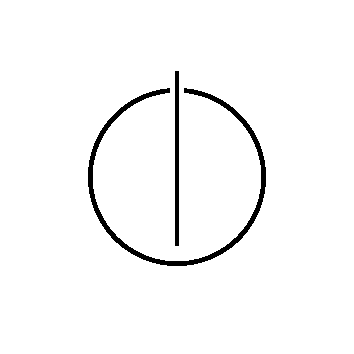
\includegraphics[width=0.3\linewidth]{gfx/infologo_BW.png}
		\end{figure}
	\end{center}
	
\end{titlepage}


% ------------------------------------  --> main title page
\begin{titlepage}
	\setlength{\evensidemargin}{22pt}
	\setlength{\oddsidemargin}{22pt}
	\pdfbookmark[0]{Titlepage}{Titlepage}
	\vspace{4cm}
	\hfill
	\begin{center}
		\oTUM{4cm}
		
		\vspace{5mm}     
		\huge DEPARTMENT OF INFORMATICS\\ 
		\vspace{0.5cm}
		\large TECHNICAL UNIVERSITY OF MUNICH\\
	\end{center}
	
	\vspace{5mm}
	
	\begin{center}
		{\Large \thesisType\ in \thesisUniversityFaculty}
		\vspace{8mm}
		
		\begin{spacing}{1.3}
			{\LARGE \thesisTitle}\\
			\vspace{8mm}
			
			{\LARGE \thesisTitleGer}\\
			\vspace{20mm}
		\end{spacing}
		
		\begin{tabular}{ll}
			\Large Author:     & \Large \thesisAuthor     \\[2mm]
			\Large Supervisor: & \Large \thesisSupervisor \\[2mm]				
			\Large Advisor:	   & \Large \thesisAdviser    \\[2mm]
			\Large Submission date:       & \Large \thesisDate
		\end{tabular}
		
		\vspace{20mm}
		
		\begin{figure}[hb!]
			\centering
			
\includegraphics[width=0.2\linewidth]{gfx/infologo.jpg}
		\end{figure}
		
	\end{center}

\end{titlepage}


% ------------------------------------  --> lower title back for single page layout
%\hfill
%\vfill
%{
%	\small
%	\textbf{\thesisName} \\
%	\textit{\thesisTitle} \\
%	\thesisSubject, \thesisDate \\
%	Reviewers: \thesisFirstReviewer\ and \thesisSecondReviewer \\
%	Supervisors: \thesisFirstSupervisor\ and \thesisSecondSupervisor \\[1.5em]
%	\textbf{\thesisUniversity} \\
%	\textit{\thesisUniversityGroup} \\
%	\thesisUniversityInstitute \\
%	\thesisUniversityDepartment \\
%	\thesisUniversityStreetAddress \\
%	\thesisUniversityPostalCode\ and \thesisUniversityCity
%}

\cleardoublepage
% !TEX root = ../my-thesis.tex
%
%************************************************
% Declaration
%************************************************
\pdfbookmark[0]{Declaration}{Declaration}
\thispagestyle{empty}

\vspace*{0.8\textheight}
\noindent
I confirm that this bachelor's thesis is my own work and I have documented all sources and material used.

\vspace{15mm}
\noindent
Munich, \thesisDate \hspace{\stretch{1}} \thesisAuthor
\newpage


%*****************************************
%*****************************************

\cleardoublepage

\pagestyle{plain}				% display just page numbers
% !TEX root = ../my-thesis.tex
%
\pdfbookmark[0]{Abstract}{Abstract}
\chapter*{Abstract}
\label{sec:abstract}
\vspace*{-10mm}

Topic modeling is a popular approach to study large document collections. It returns topics as a set of coherent words, that are usually manually labeled, regarding the concept that the top 10 words of a topic are describing. In this work is examined how the labeling of topics can be automated. Further, the internal consistency  is studied when the number of topics increases. Both approaches shall help domain experts using topic modeling for their work and understand which effect a higher or low number of topics has on the quality of the generated topics. To evaluate the results multiple datasets of online discussions regarding organic products are analyzed.

\vspace*{20mm}

{\usekomafont{chapter} Zusammenfassung}\label{sec:abstract-diff} \\

Topic modeling ist eine beliebte Methode große Textsammlung zu analysieren. Üblicherweise werden die identifizierten Themen als Liste an semantisch zusammenhängenden Wörtern dagestellt. Dieser Wörterliste wird dann manuell ein Betreff hinzugefügt. In dieser Arbeit werden unterschiedliche Ansätze verglichen, um diesen Prozess zu automatisieren. Des Weiteren wird die interne Konsistenz der Modelle bei der Veränderung der Topicanzahl analysiert. Beide Analysen sollen es Domänenexperten in Zukunft leichter machen Topic Modeling für ihre Arbeit einzusetzen. Außerdem, wird den Fachexperten dadurch ein besseres Verständnis für den Effekt der festzulegenden Topicanzahl vermittelt. Um die Ergebnisse zu überprüfen, werden die Analysen auf mehreren Datensätzen zu Onlinediskussionen über Bio-Produkten durchgeführt.
\newpage		% INCLUDE: the abstracts (english and german)
\cleardoublepage
%
% !TEX root = ../my-thesis.tex
%
\chapter*{Acknowledgement}
\label{sec:acknowledgement}
\vspace*{-10mm}

As this thesis borders between computer science and qualitative research on consumer behaviour I would like PD Dr. Georg Groh of the Research Group for Social Computing for his input during the project and Hannah Danner from the Chair of Marketing and Consumer behavior. Without their collaboration this project and thesis would not be possible. 

Special thanks got to my supervisor Dietrich Trautmann for his support and good ideas during the project and for the continuous reviews and feedback while I wrote this thesis. 

Furthermore, I would like to thank the other team members of the SocialROM project Adnan Akhundov, Ahmed Ayad, Tim Berger, Rajat Jain, Tim Berger, Vishesh Mathur and Adrian Philipp for often tedious but every-time fruitful discussions every week.

While writing this thesis the English Writing Center of the TUM was contacted several times. I especially like to thank the fellows Rose Jacobs,  Sean Rohringer, Hasan Ashraf, and Keefe Huang for reviewing my thesis.

I would like to use this opportunity to thank my parents Irina and Alexander as well as my brother Julian for their continued support during the first part of my studies. Further, I would like to thank Maria Potzner for her support while working on this project and for proof-reading this thesis. 

%jan hauffa, gerry hagerer, team members % INCLUDE: acknowledgement
\cleardoublepage
%
\setcounter{tocdepth}{2}		% define depth of toc
\tableofcontents				% display table of contents
\cleardoublepage

% --------------------------
% Body matter
% --------------------------
\pagenumbering{arabic}			% arabic page numbering
\setcounter{page}{1}			% set page counter
\pagestyle{maincontentstyle} 	% fancy header and footer

\section*{List of acronyms}
\begin{acronym}
	\setlength{\parskip}{0ex}
	\setlength{\itemsep}{1ex}
	\acro{bmel} [BMEL] {German Federal Ministry of Food and Agriculture}
	\acro{gmo} [GMO] {Genetically Modified Organism}
	
	
	\acro{lsa}	[LSA] {Latent Semantic Analysis}
	
	\acro{plsa} [pLSA] {probabilistic Latent Semantic Analysis}
	
	\acro{usda} [USDA] {U.S. Departement of Agriculture}
	\acro{svd} [SVD] {Singular Value Decomposition}
	\acro{vsm} [VSM] {Vector Space Model}	
%Maria
	\acro{ATL} [ATL] {Automatic Topic Labeling}
	\acro{BoW} [BoW] {Bag of Words}
	\acro{HLDA}[HLDA] {Hierarchical Latent Dirichlet Allocation}
	\acro{IR}	[IR] {Information Retrival}
	\acro{KL}	[KL] {Kullback Leibler}
	\acro{LDA}	[LDA] {Latent Dirichlet Allocation}
	\acro{NLP} [NLP] {Natural language processing}
	\acro{NMF} 	[NMF] {Non-negative Matrix Factorization}
	\acro{PMI} [PMI] {point-wise mutual information}
	\acro{POS} [POS] {Part-of-speech}
	\acro{tfidf} [tf-idf] {term frequency - inverse document frequency}
	
\end{acronym}
% !TEX root = ../thesis.tex
%
\chapter{Introduction}

For researchers studying consumer opinions and trends user generated content is becoming an increasingly important input. Based on the discussions underneath online editorial sources or on discussion boards social scientists can perform opinion analysis on a scale that is not possible with classical approaches.
The classical way of surveying consumers about their opinion on products or certain topics relies on voluntary questioning e.g. at supermarkets. These survey approaches have some drawbacks. First, it has to be made sure that the people questioned are representative for the larger population being studied. Second, in their response the participants might introduce a bias, since they know that they are being surveyed. Analyzing online user-generated data can help mitigate some of these drawbacks. Since the users do not know that their comments are used for opinion analyses there is less risk for bias. Further, any person has the ability to post online, which ensures that the comment sections and discussion boards contain a wide variety of opinions.

Even if user-generated content is used for qualitative studies, it is usually analyzed manually. With the huge growth of online text data, it is becoming of vital importance for social scientists to have reliable methods for fast automated analysis of such data. Among other things, researchers are interested in methods able to track topics, opinions, and sentiments in user-generated content \citep{Nikolenko2017}. Providing such a framework is the main objective of the \textit{SocialROM} project.

From a NLP perspective finding topics in large document collections is known as topic modeling. Topic models take the documents as an input and outputs topics and for every document a distribution specifying how it is composed of these topics. In topic modeling, a topic is a probability distribution over all words in the documents. By ranking the words according to their probability every topic consists of different words. However, the words of one topic refer to the same concept or theme. For example, a topic with the most probable words \textit{fish}, \textit{salmon}, \textit{wild} and \textit{seafood} refers to the \textit{fishing industry}. Each topic is a recurring theme that is discussed in the collection and is based on the co-occurrence of related words.

This project is done in cooperation with the chair of marketing research and consumer affairs at the Technical University of Munich. A part of their chair work on qualitative methods for social media analysis and opinion elicitation regarding sustainable consumption and products. Therefore, our analysis of user-generated data focuses on discussions regarding organic products. This subject is fitting since organic vs. conventional food is a widely discussed online with diverse opinions and sentiments.

In \textit{Generation 1} (\cite{Widmer2018}) firstly all data, which were relevant for our domain regarding organic food and products were scraped. Further information can be found in chapter \ref{dataset}. Then topics were generated, with the focus on finding the best topics and showing them to our domain experts. To generate the best topics different parameters for \acf{LDA} and \acf{NMF} were tried out and a method was developed to find the optimal number of topics per dataset. After creating the topics, a part of them was handed over to the domain experts and was labeled by them to evaluate, which datasets are meaningful. Based on the labels, the topic overlap  of every dataset was considered, and it was discovered, that the discussed issues from editorial articles are more similar to the topics identified in forum threads than to the topics of editorial comments and the topics from blogs are most similar to blog comments. Furthermore, the topic labels were compared with the results of a qualitative survey, where people were asked why the buy organic products. The given reasons were also reflected in the topics derived from online discussions. Analogously, to \cite{Griffiths2004} the development of topics over time was considered, to identify trends.

This thesis builds up on the topics from \textit{Generation 1}, theses were used to apply \acf{ATL} on them. The output of topic models are topics, which are represented with the top 10 words, sorted according the highest probability. It is desired, that the topics belong to a concept. For example from the top 5 words \textit{costs, price, food, product} and \textit{supermarket} it becomes apparent, that it is dealing with \textit{food prices}. Therefore, the label food prices is assigned to the topic. The label assignment has so far been only done by domain experts, which is very time consuming for them. Therefore, different procedures for the automatic allocation of labels to topics were tried out and compared, in order to relieve the domain experts or to support them in their work. This is also necessary if topic modeling is generated on a growing live corpus and new topics can be constantly added, e.g. online discussions, and the actual themes shall be shown.

After \ac{ATL} another main goal of this work is to prove the internal consistency, which means, to analyze how the topics itself and the distribution of topics on documents change when increasing the number of topics. Concretely, it shall be analyzed with different key figures whether the topics are getting specific or general and what specific and general in this context means. Furthermore, it shall be examined if the topics split up and whether this can be proven according to the top 10 words of the topic. All theses analyses shall provide domain experts the overview how topics change when increasing or decreasing the number of topics, so they can assess, which topic model is the most appropriate one for their expected results.
%\section{Research Objectives}
%	Wie baue ich darauf auf?
\section{Thesis structure}
First the methods, which were used to identify the topics are introduced in Chapter \ref{methodology}. This includes the approaches to represent the content of documents numerically and the algorithms for topic modeling with \acf{LDA} and \acf{NMF} .
In chapter \ref{dataset} we introduce the dataset and show how the data were gathered and preprocessed.
In the first half of Chapter 4, in Section \ref{automaticTL}, the possible approaches for \acl{ATL} are described and the results of applying those on our dataset are discussed. Accordingly, in the second half of Chapter 4, in Section \ref{Internal_consistency}, different key figures to measure the internal consistency are first introduced, applied and then discussed on our dataset.
Chapter \ref{future_work} completes the thesis by providing an outlook for possible future work and summarizes the thesis with the conclusion.

\newpage
\chapter{Methodology}
\label{methodology}
In this chapter the basic principles for the following chapters will be explained.
The Section \ref{sec:docrep} describes how documents can be numerically represented. Section \ref{sec:topicmodel} then will introduce the topic modeling methods \ac{LDA} and \ac{NMF} which are used in this thesis.

\section{Document representation}
\label{sec:docrep}

\subsection{Bag of Words}
The Bag of Words \ac{BoW} model serves as a numerical representation of a document, which is used as input for further \ac{NLP} tasks.
It represents the document simply by the counts for each word. The grammar and the ordering of the words are ignored, so some information is lost. The document \textit{John likes organic but Mary doesn't} and the document {Mary likes organic but John doesn't} have the same \ac{BoW} representation although these differ in context. Nevertheless, similar \ac{BoW} imply similar document content (\cite{Manning2008}). 

\subsection{Tf-Idf Weighting}
Only considering the absolute term frequency ($tf_{t,d}$) of words is not the best measure to make differentiations between documents, because not all terms are equally important. 
The term \textit{organic} appears in  224 of 239 articles in the New York Times, obviously this term can not be considered as a stop word, however it is not suitable to differentiate the articles. Therefore the effect of the frequent words is reduced by the \textit{inverse document frequency}:
\begin{equation}
idf_{d,t} = log\dfrac{N_{d}}{df_{d,t}}
\end{equation}
%$$ idf_{d,t} = log\dfrac{N_{d}}{df_{d,t}} $$
$N_{d}$ is the number of all documents in a corpus, while $df_{d,t}$ is the number of documents that contain the single term.\\
Based on the term frequency $tf_{t,d}$ and the inverse document frequency $idf_{d,t}$ we introduce the \textit{\ac{tfidf}}: 

\begin{equation}
tf-idf_{d,t} = tf_{t,d} * idf_{t,d}
\end{equation}
%$$ tf-idf_{d,t} = tf_{t,d} * idf_{t,d}$$

The \ac{tfidf} weighting has the highest score when the term occurs frequently within a small amount of documents. The score is lower when the term occurs rarely or too often in many documents (\cite{Jurafsky2009}).

\subsection{Vector space model}
The representation of documents in the same vector space is known as the vector space model. This was originally introduced for \ac{IR} operations like scoring documents on a query, document classification or clustering \cite{Salton1975}.\\
The vector space model forms with the documents \textit{$D_{i}$} and all unique terms \textit{$T_{j}$} the document term matrix \textit{C}. Each row of \textit{C} corresponds every single document of the corpus and each column the single unique terms. In \textit{$C_{ij}$} the weightings either as term frequency or \ac{tfidf} for each term over all documents is stored. \\
In Table \ref{tab:doc_term_lda} the term frequency and in Table \ref{tab:doc_term_nmf}  \ac{tfidf} is calculated from three sample documents: \textit{Doc 1: Organic is healthier then conventional food}, \textit{Doc 2: I buy organic} and \textit{Doc 3: Organic is wasted money}.
In this thesis both topic modeling algorithms take the document term matrix as input, but with different weightings. For \ac{LDA} the term frequency and for \ac{NMF} the \ac{tfidf} weighting  is used.\\
\begin{table}[h]
	\begin{tabular}{lcccccccccc}
		\toprule
		& organic & is & healthier & then & conventional & food & i &buy& wasted  & money \\ \midrule
		Doc1 & 1 	& 1  &      1      &  1   & 1 			 & 1  	& 0 &0  &  0   	&  0  \\
		Doc2 & 1 	& 0  &      0      &  0   & 0 			 & 0  	& 1 &1  &  1   	&  0  \\
		Doc3 & 1 	& 1  &      0      &  0   & 0 			 & 0  	& 0 &0  &  1    &  1   \\ \bottomrule
	\end{tabular}
	\caption[Sample term frequency matrix]{Document term matrix with term-frequency weighting as used by \ac{LDA}.}
	\label{tab:doc_term_lda}
\end{table}	

\begin{table}[h]
	\begin{tabular}{lllllllllll}
		\toprule
		& organic & is & healthier & then & conventional & food & i &buy& wasted  & money \\ \midrule
		Doc1 & 0 	& 0.45  &   0.45      &  0.45   &  	0		 & 0.34  	& 0 &0.27  &  0.45   	&  0  \\
		Doc2 & 0.65 	& 0  &      0      &  0   & 0.65			 & 0  	& 0 &0.39  &  0   	&  0  \\
		Doc3 & 0 	& 0  &      0      &  0   & 0 			 & 0 .44 	& 0.58 &0.34  &  0    &  0.58   \\ \bottomrule
	\end{tabular}
	\caption[Sample \ac{tfidf} matrix]{Document term matrix with \ac{tfidf} weighting as used by \ac{NMF}.}
	\label{tab:doc_term_nmf}
\end{table}


\section{Topic Modeling}
\label{sec:topicmodel}
Every day large amounts of information are collected and become available. The vast quantities of data make it difficult to access those information we are looking for. Therefore, we need methods that help us to organize, summarize and understand large collections of data. Topic Modeling refers to a set of methods that help us to process large document collections efficiently. A topic model takes a set of documents as the input and outputs topics, a set of recurring themes that are discussed in the collection, and the degree to which each document expresses these topics \citep{Blei2003}. The topics are the hidden thematic structure of the document collection. They are found by recurring patterns of co-occurring words.

Topic Models are based on the assumption that a document is composed of multiple topics. Any document of the text collection is a combination of all topics with different weights. Therefore, all documents of one corpus are composed of the same topics by varying their weights. The documents are modeled as a probability distribution over the topics. 

Just as documents are distributions over all topics, topics are distributions over all words in a document collection. Every word of the collection is present in every topic, however, with varying probabilities. Sorting the terms of a topic by their probability reveals a semantically meaningful interpretation.

\subsection{Latent Dirichlet Allocation}
Currently, the most used method for topic modeling is \acl{LDA}, which was introduced by \cite{Blei2003}. \ac{LDA} is a generative model, that describes how the documents are generated from existing topics. By applying inference it is possible to reverse the process and use \ac{LDA} to derive the topics from the document collection. Further, \ac{LDA} is also a probabilistic model which means that the resulting topics can be seen as a probability distribution.

The research on topic models was started by \cite{Deerwester1990} with their introduction of \ac{LSA}. \ac{LSA} was used to solve the issues of polysemy and synonymy when performing queries for information retrieval. With probabilistic \ac{LSA} (pLSA) \cite{Hofmann1999} provided a probabilistic formulation of \ac{LSA}. \ac{LDA} is an extension of pLSA to be able to model unseen documents. In pLSA the topic proportions for every document need to be known, which makes it unable to model documents outside the training set. In \ac{LDA} the topic proportions for every document are derived from a Dirichlet distribution, thus enabling it to generalize to documents outside the training collection.

After the successful introduction to analyze large document collections, \ac{LDA} was also applied in other domains such as computer vision to classify \citep{Fei-Fei2005} and build hierarchies of images \citep{Li2010}. In fact, the method was independently discovered by \cite{Pritchard2000} in their field of evolutionary biology to study population genetics. For the interested reader, \cite{Jelodar2017} presents a literature study on extensions of \ac{LDA} and applications to various datasets.

As described above \ac{LDA} assumes a generative process how the documents of a corpus arose from existing topics. We first describe the generative process before explaining how it can be reversed to derive topics from existing documents.

\ac{LDA} draws the per-document topic distribution and the topics themselves from a  Dirichlet distribution. Therefore, before explaining \ac{LDA} the Dirichlet distribution is introduced. 

The Dirichlet distribution can be seen as a distribution over distributions. When sampling from a k-dimensional Dirichlet distribution one receives a discrete distribution over k elements. This is visualized in Figure \ref{fig:dirichlet1}. Each distribution represents a draw from a 3-dimensional Dirichlet distribution.

Further, the Dirichlet distribution can be parametrized by $\alpha$. The parameter describes how the probability mass of the Dirichlet distribution is distributed over the k-elements. When drawing from a Dirichlet with a high alpha parameter the probabilities for each element of the drawn discrete distribution are roughly the same. When drawing from a Dirichlet with a small alpha, the probability mass of the resulting discrete distribution is divided among a few highly probable elements. Visually, a high $\alpha$ value leads to a distribution as shown on the left of Figure \ref{fig:dirichlet1}. A low value would lead to distributions as shown on the right.

\begin{figure}
	\centering
	
		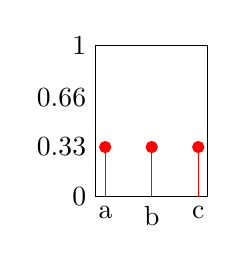
\begin{tikzpicture}
		\begin{axis}[
		width = 3cm,
		height = 3.5cm,
		symbolic x coords={a,b,c},
		xtick=data,
		ytick={0, 0.33, 0.66, 1},
		ymax=1,
		ymin=0,
		ytick style={draw=none},
		xtick style={draw=none}		
		]
		\addplot+[ycomb, color=red, mark options={red}] coordinates {(a,0.33) (b,0.33) (c,0.33)};
		\end{axis}
		\end{tikzpicture}
		\quad
		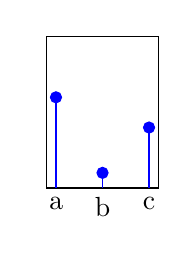
\begin{tikzpicture}
		\begin{axis}[
		width = 3cm,
		height = 3.5cm,
		symbolic x coords={a,b,c},
		xtick=data,
		yticklabels={,,},
		ymax=1,
		ymin=0,
		ytick style={draw=none},
		xtick style={draw=none}		
		]
		\addplot+[ycomb, color=blue, mark options={blue}] coordinates {(a,0.6) (b,0.1) (c,0.4)};
		\end{axis}
		\end{tikzpicture}
		\quad
		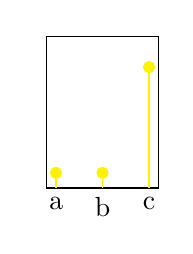
\begin{tikzpicture}
		\begin{axis}[
		width = 3cm,
		height = 3.5cm,
		symbolic x coords={a,b,c},
		xtick=data,
		ymax=1,
		ymin=0,
		ytick style={draw=none},
		xtick style={draw=none},
		yticklabels={,,}		
		]
		\addplot+[ycomb, color=yellow, mark options={yellow}] coordinates {(a,0.1) (b,0.1) (c,0.8)};
		\end{axis}
		\end{tikzpicture}
	\caption[Discrete distributions drawn from a 3-dimensional Dirichlet distribution]{Discrete distributions drawn from a 3-dimensional Dirichlet distribution. Adapted from \cite{Widmer2018}}
	\label{fig:dirichlet1}	
\end{figure}

Figure \ref{fig:dgmlda} represents \ac{LDA} as a graphical model. The grey nodes indicate observed variables, in this case the words $w$ of the documents. All white nodes are hidden variables that have to be derived. In topic modeling the hidden variables are the topic assignment $z_{w,d}$ of each word position $n$ in document $d$, the topic distribution $\theta_d$ for document $d$ and the word distribution $\phi_z$ for topic $z$. $\alpha$ and $\beta$ are hyper- parameters for the Dirichlet distribution on the per-document topic distribution and per-topic word distribution respectively.
With the introduced notation the generative process underlying \ac{LDA} can be described as follows:

\begin{itemize}
	\item From a Dirichlet distribution parametrized by $\alpha$ draw a multinomial distribution $\theta_d$ representing the topic proportions of document $d$. 
	\item For each word position $n$ in document $d$ choose a topic of the multinomial per-document topic distribution $\theta_d$. The chosen topic is the topic assignment $z_{n,d}$.
	\item From a Dirichlet distribution parametrized by $\beta$ draw a multinomial distribution $\phi_z$ representing the word proportions for topic $z$.
	\item The word $w$ at position $n$ in document $d$ is then drawn from the topic $z$. 
\end{itemize}

By applying this procedure for all documents and words we can generate the documents from existing topics. To derive the topics from existing documents we need to estimate the document-topic proportions $\theta$, the topics $\phi$ and the assignment of words to topics $z$ given the Dirichlet priors $\alpha$ and $\beta$ and the word of the documents $w$. This can be formulated as:
\begin{equation}
P(\theta, \phi, z| w, \alpha, \beta) = \frac{P(\theta, \phi, z, w |\alpha, \beta)}{P(w |\alpha, \beta)} 
\end{equation}

This fraction, however, is intractable to compute. Therefore, several approaches exist, such as Gibbs Sampling \citep{Griffiths2002}, Variational Inference \citep{Blei2003} or Expectation Propagation \citep{Minka2002}, to approximate the topic-term and document-topic distributions.

\begin{figure}
	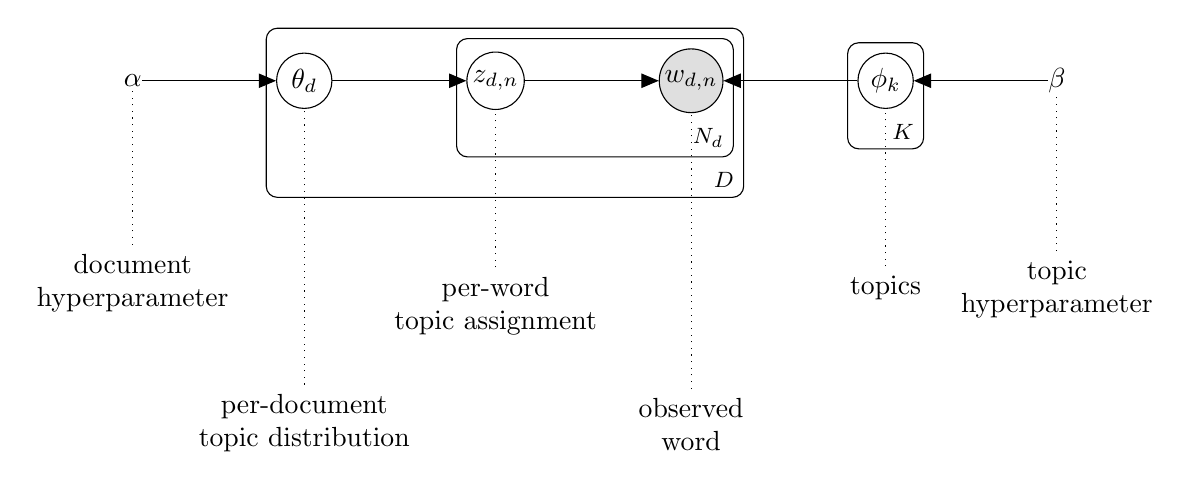
\begin{tikzpicture}[x=1.7cm,y=1.8cm]
	
	% Nodes
	\node[obs] (W) {$w_{d,n}$} ; 
	\node[latent, left =of W] (Z) {$z_{d,n}$} ; 
	\node[latent, left =of Z] (TH) {$\theta_d$} ; 
	\node[const, left =of TH] (AL) {$\alpha$} ; 
	\node[latent, right =of W] (PH) {$\phi_k$} ; 
	\node[const, right =of PH] (BE) {$\beta$} ; 
	
	% Edges
	\edge {Z} {W} ; 
	\edge {TH} {Z}; 
	\edge {AL} {TH};
	\edge {PH} {W};
	\edge {BE} {PH};

	%Plates
	\plate {topicsPlate} {(PH)} {$K$} ; 
	\plate {wordsPlate} {(W) (Z)} {$N_d$} ; 
	\plate {documentsPlate} {(wordsPlate) (TH)} {$D$}
	
	%Description
	\node[ below= 2cm of AL, align=center] (A) {document\\hyperparameter} ;
	\node[ below= 3.5 cm of TH, align=center] (DTH) {per-document  \\topic distribution} ;
	\node[ below= 2cm of Z, align=center] (DZ) {per-word \\ topic assignment} ;
	\node[ below= 3.5cm of W, align=center] (DW) {observed \\ word} ;
	\node[ below= 2cm of PH, align=center] (DPH) {topics} ;
	\node[ below= 2cm of BE, align=center] (DBE) {topic \\ hyperparameter} ;
	\draw[dotted] (A) -- (AL) ;
	\draw[dotted] (DTH) -- (TH) ;
	\draw[dotted] (DZ) -- (Z) ;
	\draw[dotted] (DW) -- (W) ;
	\draw[dotted] (DPH) -- (PH) ;
	\draw[dotted] (DBE) -- (BE) ;
	\end{tikzpicture}
	

	\caption[Graphical model of \ac{LDA}]{Graphical model of \ac{LSA}. Adapted from \cite{Widmer2018}}
	\label{fig:dgmlda}
\end{figure}


\subsection{Non negative Matrix Factorization}

Apart from the probabilistic methods as described above, linear methods, such as \acl{NMF} have proven useful for topic modeling. \ac{NMF} was introduced by \cite{Lee1999} as a method for dimensionality reduction. They show that their method can lead to a lower dimensional parts-based representation with naturally interpretable components. When applied on a set of facial images, the parts resemble different portions of a human face. The original facial images can be reconstructed by combining the parts. This approach can also be applied on a set of textual documents. In this case the parts-based representation are the semantic topics of the documents and the documents can be reconstructed by combining the topics.

\ac{NMF} requires that the original data is non-negative. This is the case for the previously presented applications in computer vision and text mining. The pixel values of images or term counts of documents are always positive. It is also typical to data in other fields that they are non-negative. Therefore, \ac{NMF} was also successfully applied in spectral analysis \citep{Pauca2006} and bio-informatics\citep{Brunet2004}.

Formally, \ac{NMF} can be described as follows. Given a non-negative matrix $C \in \mathbb{R}_{\geq 0}^{n\times m}$ and a rank desired $k < min(m,n)$ find two non-negative matrices $W \in \mathbb{R}_{\geq 0}^{n \times k}$ and $H \in \mathbb{R}_{\geq 0}^{k \times m}$ so that the reconstruction error is minimized:
\begin{equation}
\min_{W,H} ||C - WH||_F
\end{equation}
In this case, the reconstruction error is measured by the Frobenius norm, which is an extension of the Euclidean form on matrices. The output and input of \ac{NMF} is similar to \ac{LDA}. Matrix $C$ is the original document term matrix whereas the matrices $W$ and $H$ represent the topic term respectively the document topic matrix. For every document $c$ there is a corresponding column $h$ in the document topic matrix $H$. The column contains the weights for each topic (columns of $W$) for this specific document. Thus, the document $c$ is modeled as a linear combination of the columns of $W$:
\begin{equation}
c \approx Wh
\end{equation}.
The similarity of \ac{LDA} and \ac{NMF} in terms of matrix factorization is evident from Figure \ref{fig:comparison}. However, there is an important difference in the interpretation of  the values in the generated matrices. With \ac{LDA} the outputted document-topic and topic-term matrices are probability distributions. \ac{NMF}, however, has no probabilistic interpretation and while returned values represent topic or term weights they do not necessarily sum up to 1. To circumvent this difference the output of \ac{NMF} was normalized. 

\begin{figure} 
	\centering
			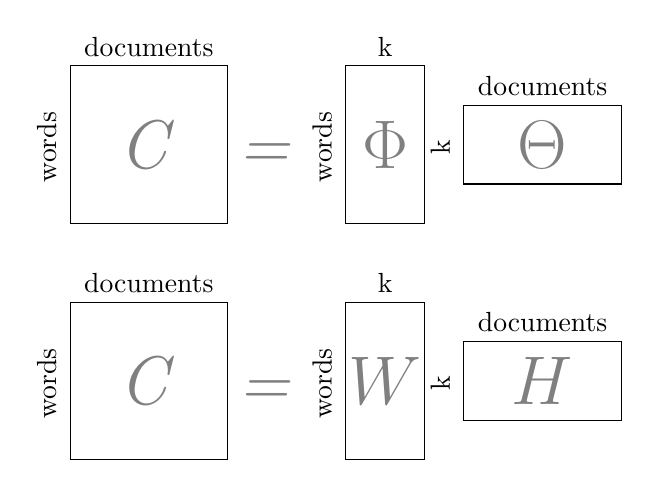
\begin{tikzpicture}
			
			% LDA
		 	\draw (0, 0) rectangle (2, 2);
		 	\node [above] at (1, 2) {documents};
		 	\node [right, rotate=90] at (-0.3, 0.4) {words};
		 	\node at (1, 1) {\Huge \color{gray} \textit{C}};
		 	\node at (2.5, 0.85) {\Huge \color{gray} \textit{=}};
		 	
		 	\draw (3.5, 0) rectangle (4.5, 2);
		 	\node [above] at (4, 2) {k};
		 	\node [right, rotate=90] at (3.2, 0.4) {words}; 
		 	\node at (4, 1) {\Huge \color{gray} $\Phi$};
		 	
		 	\draw (5, 0.5) rectangle (7, 1.5);
		 	\node [above] at (6, 1.5) {documents};
		 	\node [right, rotate=90] at (4.7, 0.75) {k}; 
		 	\node at (6, 1) {\Huge \color{gray} $\Theta$};
		 	
		 	% NMF
		 	\draw (0, -3) rectangle (2, -1);
		 	\node [above] at (1, -1) {documents};
		 	\node [right, rotate=90] at (-0.3, -2.6) {words};
		 	\node at (1, -2) {\Huge \color{gray} \textit{C}};
		 	\node at (2.5, -2.15) {\Huge \color{gray} \textit{=}};
		 	
		 	\draw (3.5, -3) rectangle (4.5, -1);
		 	\node [above] at (4, -1) {k};
		 	\node [right, rotate=90] at (3.2, -2.6) {words}; 
		 	\node at (4, -2) {\Huge \color{gray}  $W$};
		 	
		 	\draw (5, -2.5) rectangle (7, -1.5);
		 	\node [above] at (6, -1.5) {documents};
		 	\node [right, rotate=90] at (4.7, -2.25) {k}; 
		 	\node at (6, -2) {\Huge \color{gray} $H$};
	
\end{tikzpicture}
		 	

	\caption[Similarity of LSA and NMF from the perspective of matrix decomposition]{Showing the similarity of \ac{LDA}, and \ac{NMF} from the perspective of matrix decomposition. Adapted from \cite{Steyvers2007a}.}
	\label{fig:comparison} 
\end{figure} 

\chapter{Dataset}
\label{dataset}
In order to identify and analyze the consumers decisions in context of sustainable food we need a large dataset, which consists of different sources to capture the various opinions and discussion topics of the large population.
The following chapter summarizes how the relevant datasets of editorial resources, personal blogs and discussion boards were selected and preprocessed in \textit{Generation 1} and which changes were made.
Afterwards it is described how the topics of the datasets were identified.
Based on already existing and new generated topics together with the scraped datasets, the following chapters presents further analysis and additional insights.

\section{Data collection}
To gather a wide rage of opinions towards sustainable food and the variation of discussion topics over time, different datasets such as online editorial news sites, blogs and discussion boards were considered in the period from January 2007 until November 2017. These datasets are all public and without any charge available  online. Additionally, the user generated data, such as comments under articles or in forums, can be posted by using a pseudonym and the users do not know their data will be studied. This reduces the potential of response bias, which is usually present when performing surveys or experiments.

Online outlets of supra-regional print press, national print press \citep{IVW2018}\footnote{only an example German national print press} and the news sites \citep{AGOF2018}\footnote{only an example German news sites} were selected  according to the highest reach by the Domain experts. Blogs and forums were selected with the help of snowball technique, meaning Domain experts` colleagues identified further sustainable blogs or forums. This kind of data were selected for Germany, Austria, Swiss and the US.

After the selection, the chosen datasets were automatically scraped and examined for terms like \textit{bio Lebensmittel}, \textit{ bio Landwirtschaft} for the German and terms like \textit{organic, organic food, organic agriculture}, and \textit{organic farming} for the English language using site`s internal search engines or Google search, which offers the option to search for sites within a domain. Nevertheless, still non relevant data like recipes, product presentations, and stock market information remained. These were kicked out by the binary Naive Bayes classifier, which was trained on 1000 random articles\footnote{contains the title, text and text of 100 comments}, that were labeled either as relevant or not by the Domain experts.
The final collection stored in a JSON schema and the list of all sources and their percentage of relevant articles together with other descriptive statistics can be found in Appendix \ref{app:descriptiv_stats}.

\section{Data processing}
\label{data:preprocessing}
For applying further \ac{NLP} tasks, the extracted dataset was transformed by using several pre-processing tasks: First, the texts were tokenized and lowercased. Then all common words including numbers and punctuations were removed and Emails and Url`s were replaced by <EMAIL> and <URL> tags. Second, the remaining tokens were lemmatized, so that the inflections of words were replaced by their basic form. Third, the texts were examined for collocations, which are co-occuring words like \textit{Stiftung Warentest} or \textit{Whole Foods},  with a Gensim library \footnote{https://radimrehurek.com/gensim/index.html}. For the lemmatization and tokenization the Spacy library \footnote{https://spacy.io} was used.
Additionally, in this project \ac{POS}-Tagging was applied to the texts, which is a process marking up the words to a particular part of speech, to facilitate the \ac{ATL} in chapter \ref{automaticTL}. 

\section{Final Datasets}
Before reporting the datasets itself, the definition of text types will be described, which were introduced because of the different content and language style. 
All data referring to a main text of a side are called \textit{editorial articles} and the comments under the editorial articles are called \textit{editorial comments}. The term \textit{Forum} includes the initial question and the comments under it.
In this thesis the blogs, which were split in editorial and comments, were neglected, because the amount of data and context quality was to low.

We created two different final datasets where the frequent words, occurring over 90\% in a document, and the infrequent words, occurring under 0,05\%, were kicked out.
The first dataset \label{chris:daten} consists of editorial articles, editorial comments and forums. The final number of documents and amount of words is listed in Table \ref{tab:editorial_forum}. The second dataset consists of editorial articles and the summarized comments from the editorials and forums. This is shown in Table \ref{tab:editoria_comments}. Both datasets were built for the German and English language. 

%editorial and forum
 	\begin{table}[h]
	\begin{tabular}{llccc}
		\cmidrule{3-5}
		&	& \multicolumn{2}{c}{Editorials} & \multirow{2}{*}{Forums} \\
		\cmidrule(r){3-4}
		&	 & articles & comments &  \\
		\midrule
		\multirow{2}{*}{German} &	 \# documents & 4730	& 1782	& 641	\\
		&	\# words & 5239	& 15413	& 7361	\\
		\midrule
		\multirow{2}{*}{English} &	 \# documents & 2345	& 441	& 3274	\\
		&	\# words & 6254	& 11948	& 5970	\\
		\bottomrule
	\end{tabular}
	\caption[Number of documents and vocabulary size for Editorials and Forums]{The number of documents and vocabulary sizes for Editorials and Forums of the German and English datasets.}
	\label{tab:editorial_forum}
	\end{table}

%editorial articles and summarized comments
	\begin{table}[h]
		\begin{tabular}{llcc}
			\cmidrule{3-4}
			&	& Editorial articles & Comments \\
			\midrule
			\multirow{2}{*}{German} &	 \# documents & 4730	& 2423	\\
			&	\# words & 5239	& 22774	\\
			\midrule
			\multirow{2}{*}{English} &	 \# documents & 2345	& 3715	\\
			&	\# words & 6254	& 17918	\\
			\bottomrule
		\end{tabular}
		\caption[Number of documents and vocabulary size for Editorial articles and Comments]{The number of documents and vocabulary sizes for Editorial articles and Comments of the German and English datasets.}
		\label{tab:editoria_comments}
	\end{table}

\section{Topic Generation}
The complete dataset not only includes the texts but also topics, that were identified as part of \textit{Generation 1}. These topics were generated separately by language and text type. Since we merged comments underneath editorial articles and forums, we generated new topics based on the same parameter and the same approach to select the number of topics.
Generating qualitative topics depends on the hyper parameters $\alpha$ and $\beta$ for \ac{LDA} and the topic number for \ac{LDA} and \ac{NMF}. The domain and the documents influence the optimal values for the hyper parameters. Therefore, in \textit{Generation 1}, the $\alpha$ and  $\beta$ were determined by analyzing the topic coherence and the perplexity of the topics. The asymmetric $\alpha$ and symmetric $\beta$ = 0.01 were considered as the best values. These were used to generate the previous topics and the new ones for summarized comments.
Obtaining the best topic number for each dataset multiple Topic Models were trained for a range of different number of topics with \ac{LDA} and \ac{NMF}. The following steps describe the process to estimate the optimal number of topics for a language, dataset and algorithm e.g. English Comments with \ac{NMF}:
\begin{enumerate}
	\item For every Topic Model with different topic numbers a plot was generated, see Figure \ref{fig:mean}.
	The x-axis shows the values for the most probable topic for every single  document while the y-axis shows the counted documents where the topic occurs.
	\item In each plot the mean of the x-axis values was calculated. Afterwards the means of all plots were averaged and used as a threshold in the next step.
	\item The number of documents was summed up if the probability of the topics was greater then the threshold. The sum was calculated for every Topic Model and plotted in Figure \ref{fig:topic number}.
	\item The point where the curve flattens, was taken as the optimal topic number.
\end{enumerate}
	
\begin{figure}
	\centering
	\begin{minipage}[b]{0.5\textwidth}
		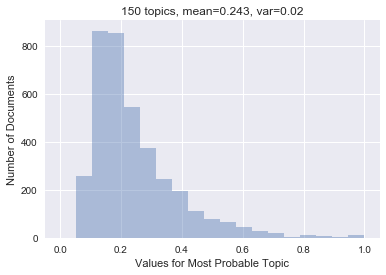
\includegraphics[width=7cm]{gfx/Hyperparams/150topics_English_nmf.png}
		\caption{Count of the value of the most probable topic, summed over all topics.}
		\label{fig:mean}
	\end{minipage}%
	\begin{minipage}[b]{0.5\textwidth}
		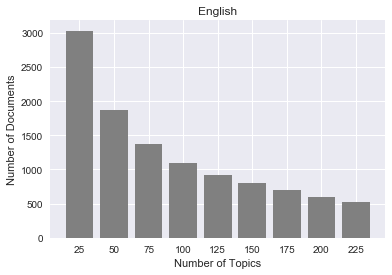
\includegraphics[width=7cm]{gfx/Hyperparams/English_nmf_Comments.png}
		\caption{Number of documents the topics are expressed above the threshold}
		\label{fig:topic number}
	\end{minipage}
\end{figure}	

After finding the appropriate topic number, the Topic Models generated with \ac{NMF} and \ac{LDA} for the same dataset were inspected manually. The domain experts labeled the topics and the Topic Model with the higher number of labels was chosen. The final selection of the Topic Models including also Topic Models with summarized comments is shown in Table \ref{tab:finaltopics_editorial_forums}.


\begin{table}[h]
	\centering
	\makebox[0pt][c]{\parbox{1.0\textwidth}{%
		\begin{minipage}[b]{0.5\textwidth}
			\begin{tabular}[b]{lcc}
				\cmidrule{2-3}  & Editorial articles & Comments
				\\ \midrule
				German    & \textbf{190} &    \textit{125}       \\
				English    & \textbf{130}  &      \textit{125}       \\ 
				\bottomrule
			\end{tabular}
		\end{minipage}
		\begin{minipage}[b]{0.5\textwidth}
			\begin{tabular}[b]{lccc}
				\cmidrule{2-4}  & \multicolumn{2}{c}{Editorials} & \multirow{2}{*}{Forums} \\
				\cmidrule(r){2-3}
				\cmidrule(r){2-3}
				& articles     &    comments       &                         
				\\ \midrule
				& \textbf{190} &  \textit{170}    &      \textit{170}       \\
				& \textbf{130} &  \textit{170}    &      \textbf{110}       \\ 
				\bottomrule
			\end{tabular}
		\end{minipage}
\vspace{1pt}
\caption[Final number of topics for Editorials and Forums]{The optimal number of topics for Editorials and Forums. \\
	\textit{Italic} denotes \ac{NMF} and \textbf{bold} numbers denote \ac{LDA}.}
\label{tab:finaltopics_editorial_forums}
}}
\end{table}
\newpage
\chapter{Experiments and Evaluation}
\section{Topic ranking}


\subsection{Related work}
-Topic Signi¯cance Ranking of LDA Generative
Models

\subsection{Topic Coherence}
Actually, good topics were determined from domain experts after topic labeling. The topics were labels from three labelers. If only one labeler or none of the labelers could assign a label the label was ranked with relevance score 0 otherwise with 1.


Actually, topic ranking with the help of labeling the topics 


topics. However, not all the es-
timated topics are of equal importance or correspond to genuine themes
of the domain. Some of the topics can be a collection of irrelevant or
background words, or represent insigni¯cant themes.
identify and distinguish
junk topics from legitimate ones, and to rank the topic signi¯cance. The

The setting of the number of latent variables K is extremely critical and
directly e®ects the quality of the model and the interpretability of the estimated
topics. Models with very few topics would result in broad topic de¯nitions that
could be a mixture of two or more distributions.
topics is low in signi¯cance and
often meaningless.


%document topic matrix theta
\subsection{Summed Theta $\theta$}
%select topics that occure in most of the documents
%sumed up theata over all documents and rank it according to the highest
%TODO: was mit doc 1 = 80 und doc 2 = 20
\subsection{Iter-rater reliability}
%iter rater für alle datasets

%de_edit_art:  0.8225175207062891
%
%de_edit_comm:  0.853215284249767
%
%de_forum:  0.818621523579202
%
%en_edit_art:  0.828312425602051
%
%en_edit_comm: 0.4876510772464529
%
%en_forum: 0.8628132430949332
%
%The topics were labeled manually by three labelers. To evaluate the iter-rater reliability for every dataset the \textit{Fleiß kappa}\footnote{https://en.wikipedia.org/wiki/Fleiss\%27_kappa} was used. Fleiß kappa is a statistical measurement 

%TODO genaue berechnung von fleiss kappa?
Fleiss' kappa (named after Joseph L. Fleiss) is a statistical measure for assessing the reliability of agreement between a fixed number of raters when assigning categorical ratings to a number of items or classifying items.
cohens kapp only for max 2raters

%If the raters are in complete agreement then κ = 1   {\displaystyle \kappa =1~} \kappa =1~. If there is no agreement among the raters (other than what would be expected by chance) then κ ≤ 0 {\displaystyle \kappa \leq 0} \kappa \leq 0. 

%< 0 	Poor agreement
0.01 – 0.20 	Slight agreement
0.21 – 0.40 	Fair agreement
0.41 – 0.60 	Moderate agreement
0.61 – 0.80 	Substantial agreement
0.81 – 1.00 	Almost perfect agreement

he value pj is the proportion of all assignments (raters * number of topics) that were made to the jth category.

k:The value is between 0 and 1.
The higher the value the better is the agreement between the raters.

N = anzahl an topics.
n = anzahl an labelers (3)
k = anzahl an labels
%%rel work
% sumeed up theta
% vis doc topic visualization
%coherence

\subsubsection{Coherence}
Hallo @Maria Potzner. Meinem Eindruck nach hat der Score wenig Aussagekraft. Man kann kaum sagen, dass Topics, die weiter oben stehen "besser" sind als jene, die weiter unten stehen. Einen Treshold festzulegen ist daher erst recht nicht möglich.

SUMMED Theta:ab hier die topics rauswerfen", ein solcher Treshold wäre dann auch bei jedem der 6 models untschiedlich. Die topics am Ende kommen eben seltener vor, es sind aber trotzdem sehr sinnvolle auch am Ende dabei, während am Anfang auch einige "non-sense" topics stehen, zB Zeile 17 letztes Tabellenblatt.

Also was für mich im Moment am besten erscheint wäre tatsächlich eine Selektion und Labelling durch den Domain expert. Dann kann man z.B. noch ein Ranking nach Topic-Häufigkeit machen.



\newpage

\section{Automatic Topic Labeling}
\label{automaticTL}
Topic Models are used to discover latent topics in a corpus to help to understand large collections of documents. These topics are multinomial distributions over all words in a corpus. Normally, the top terms of the distribution are taken to represent a topic, but these words are often not helpful to interpret the coherent meaning of the topic. Especially, if the person is not familiar with the source collection. For example, for the topic \textit{price, \$, cost, foods, store, product, brand, low, supermarket, good} a  suitable label is \textit{food prices}.

With the help of \acf{ATL} we want to reduce the cognitive overhead of interpreting these topics and, therefore, facilitate the interpretation of the topics.
Of course, the topics can be labeled manually by domain experts, but this method is time consuming if there are hundreds of topics. Additionally, the topic labels can be biased towards the users opinion and the results are hard to replicate. 

We are working with domain specific data dealing with organic food. To generate meaningful labels we can not make use of human turks because we need domain experts who are proficient in this area. Therefore, we submitted the topics to our domain experts to label them. But only 50 of the generated topics, ranked according to the importance in a corpus, for each dataset were handed in, in order to not burden them, since this process is very time-consuming. The datasets were labeled by three labelers who tried to find a suitable label, which captures the meaning of the topic and is easily understandable. After labeling, the three labels of a topic were compared and a final label was set. If at least two labelers had the same label, this was taken as the final one. If the given labels were not comparable, no label was set at all. 

To relieve our domain experts in the following chapter two approaches for \ac{ATL} are described. In Section \ref{sec:intrinsic} an intrinsic method was used, which is only working on texts and topics from our datasets to generate the labels according \cite{Mei2007}. Section \ref{sec:extrinsic} describes an extrinsic approach by using a lexical database for the English language called \textit{Wordnet} to label the topics.

\subsection{Related work}                                                
\label{sec:relWorl: atl}
\textit{\cite{Lau2011}} generated a label set,called primary candidate labels, out of article titles, which were found in Wikipedia or Google by searching the top N words from topics. Afterwards, these labels were chunkized and n-grams were generated. Theses secondary candidate labels were then filtered with the \textit{related article conceptual overlap} (RACO), that removed all outlier labels, such as stop words. Then the primary and secondary candidate labels were ranked by features such as \ac{PMI}, used for measuring association, and the student’s t test. The results were measured with the mean absolute error score for each label, which is an average of the absolute difference between an annotator’s rating and the average rating of a label, summed across all labels. The score lay between 0.5 and 0.56 on a scale from 0 to infinity.

On topics from Twitter \textit{\cite{Zhao2011}} used  a topic context sensitive Page Rank to find keywords by boosting the high relevant words to each topic. These keywords were taken to find keyword combinations (key phrases) that occur frequently in the text collection. The key phrases were ranked according to their relevance,i.e. whether they are related to the given topic and discriminative, and interestingness, the re-tweeting behavior in Twitter. To evaluate the keywords Cohen’s Kappa was used to calculate the iterrater reliability between manually and automatically generated key phrases. The Cohen’s Kappa coefficient was in the range from 0.45 to 0.80, showing good agreement.

\textit{\cite{Allahyari2015}} created a topic model OntoLDA which incorporates an ontology into the topic model and provides \ac{ATL} too. In comparison with \ac{LDA}, OntoLDA has an additional latent variable, called concept, between topics and words. So each document is a multinational distribution over topics, each topic is a multinomial distribution over concepts and each concept is a multinomial distribution over words.  Based on the semantics of the concepts and the ontological relationships among them the labels for the topics are generated in followin steps:
\begin{enumerate}
	\item construction of the semantic graph from top concepts in the given topic
	\item selection and analysis of the thematic graph (subgraph form the semantic graph)
	\item topic graph extraction from the thematic graph concepts
	\item computation of the semantic similarity between topic and the candidate labels of the topic label graph
\end{enumerate}
The top N labels were compared with the labeling from \textit{\cite{Mei2007}} by calculating the precision after categorizing the labels into good and unrelated. The more labels were generated for a topic the more imprecise they got but the preciser \textit{\cite{Mei2007}} labels were.

\textit{\cite{Hulpus2013}} made use of the structured data from DBpedia, that contains structured information from Wikipedia. For each word of the topic the Word-sense disambiguation (WSD) chose the correct sense for the word from a set of different possible senses. Then a topic graph was obtained form DBpedia consisting of the closest neighbors and the links between the correct senses. Assuming the topic senses which are related, lie close to each other, different centrality measures were used and evaluated manually to identify the topic labels. The final labels then were compared to textual based approaches and the precision after categorizing the labels into good and unrelated was calculated.

\cite{Kou2015} captured the correlations between a topic and a label by calculating the cosine similarity between pairs of topic vectors and candidate label vectors. Continuous bag of words (CBOW), Skip-gram and Letter Trigram Vectors were used. The candidate labels were extracted from Wikipedia articles that contained at least two of the top N topic words. The resulting labels for the different vector spaces were compared to automatically generated gold standard labels, representing the most frequent chunks of suitable document titles for a topic. The final labels were ranked by human annotators,too, and were considered as a better solution than the first word of the top N topic words. 

For topics and preprocessed Wikipedia titles \textit{\cite{Bhatia2016}} used word and title embeddings. To generate title embeddings doc2vec and word2vec were used to obtain fine-grained labels (doc2vec) or generic labels (word2vec). Given a topic, the relevance of each title embedding was measured based on the pairwise cosine similarity with each of the word embeddings for the top-10 topic terms. The sum of of the relevance of doc2vec and vec2doc served as ranking for the labels. The results were evaluated the same way as like in \cite{Lau2011}.

\textit{\cite{Magatti2009}} used a given tree-structured hierarchy from the Google Directory to generate candidate labels for the topics. These were compared to the topic words by applying different similarity measures. The most suitable label was then selected by exploiting a set of labeling
rules. This approach is applicable to any topic hierarchy summarized by a tree.

\textit{\cite{Mei2007}} generated labels based on the texts collection and their related topics by chunking and building n-grams. They approximated the distribution for the labels and compared these to the distribution of the topic by calculating the \ac{KL} divergence. To maximize the mutual information between the label and the topic distributions the calculated divergence has to be minimized. Three human assessors measured the results and found out that the final labels are effective and robust although applied on different genres of text collections. 


\subsection{Intrinsic Topic Labeling}
\label{sec:intrinsic}
The intrinsic topic labeling is based only on a text collection and therefrom extracted topics.It does not use any external ontologies or embeddings. Because \textit{\cite{Mei2007}} were the only ones who generated topic labels by using an intrinsic approach, we decided to apply their \ac{ATL} on our data, using an implementation from Github\footnote{https://github.com/xiaohan2012/chowmein}. The implementation was adapted to our data and instead of using their preprocessing ours was used.

In their paper \textit{\cite{Mei2007}} consider noun phrases and n-grams as candidate labels and use \acf{POS}-tags to extract the labels according to some grammar from the text collection. We apply the n-grams approach to select (NN - NN) or (JJ - NN) English and (NN -NN) or (ADJD - NN) German bi-grams as suitable labels for the topics.

The candidate labels were ranked by their semantic similarity to the topic distribution $\theta$. To measure the semantic relevance between a topic and a label \textit{l} a distribution of words \textit{w} for the label $p(w|l)$ was approximated by including a text collection \textit{C} and a distribution $p(w|l,C)$ was estimated, to substitute $p(w|l)$. Then the \acf{KL} divergence $D(\theta||l)$ was applied to calculate the closeness between the label and the topic distribution $p(w|\theta)$. So the \ac{KL} divergence served to capture how well the label fits to the topic. If the two distributions perfectly match each other and the divergence is zero we have found the best label. 
The relevance scoring function of \textit{l}  to $\theta$ is defined as the negative \ac{KL} divergence $-D(\theta||l)$ of $p(w|\theta)$ and $p(w|l)$ and can be rewritten as follows by including \textit{C}:
\begin{align}
\begin{split}
	Score(l,\theta) = &-D(\theta||l) =
	-\sum_{w} p(w|\theta)log\frac{p(w|\theta)}{p(w|l)}\\ =
	&-\sum_{w} p(w|\theta)log\frac{p(w|C)}{p(w|l,C)} -\sum_{w} p(w|\theta)log\frac{p(w|\theta)}{p(w|l)}\\ &-\sum_{w} p(w|\theta)log\frac{p(w|l,C)}{p(w|l)} \\ =
	&-\sum_{w} p(w|\theta)log\frac{p(w,l|C)}{p(w|C) p(l|C)} -D(\theta||C)\\ &-\sum_{w} p(w|\theta)log\frac{p(w|l,C)}{p(w|l)}\\  =
	&-\sum_{w} p(w|\theta) PMI(w,l|C)-D(\theta||C) + Bias(l|C) 
\end{split}
\end{align}
We can see that the relevance scoring function consists of three parts. The first part represents the expectation of \ac{PMI} $E_{\theta}(PMI(w,l|C))$ between \textit{l} and the words in the topic model given the context \textit{C}, the second part is represented by the \ac{KL} divergence between $\theta$ and \textit{C} and the third part can be viewed as a bias using context
\textit{C} to infer the semantic relevance \textit{l} and $\theta$. This bias can be neglected for our data because we have used the same text collection for  producing the topics and the labels. The same applies to the second part, because the \ac{KL} divergence has the same value for all candidate labels. Therefore, we rank the topic labels with 
\begin{equation}
Score(l,\theta) = E_{\theta}(PMI(w,l|C))
\label{Mei:Scoring}
\end{equation}

\begin{figure}[t]
	\begin{minipage}[t]{0.5\textwidth}
		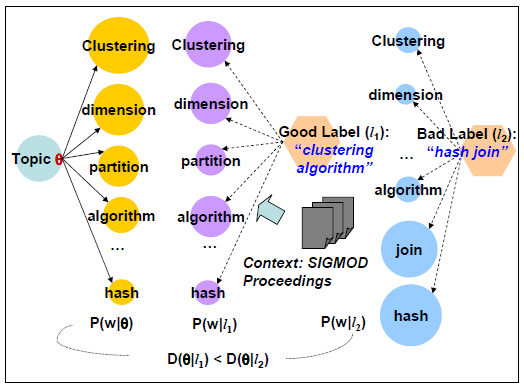
\includegraphics[width=\textwidth]{gfx/Mei/MeiGoodLabel.png}
	\end{minipage}
	\begin{minipage}[t]{0.512\textwidth}
		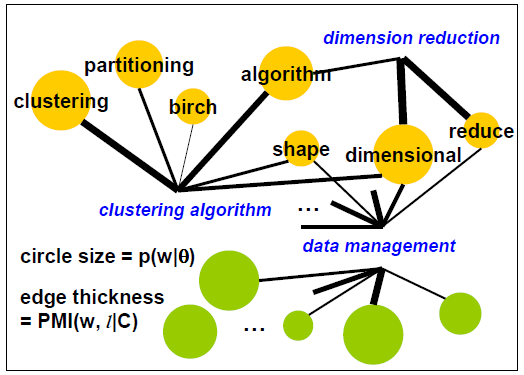
\includegraphics[width=\textwidth]{gfx/Mei/MeiScoring.png}
	\end{minipage}
	\caption[Relevance scoring function for \ac{ATL}]{Relevance scoring function for \ac{ATL}. Adapted from \cite{Mei2007}}
	\label{pic:ScoringFunction}
\end{figure}

The relevance scoring function is also described visually in Figure \ref{pic:ScoringFunction}. The circles represent the probability of terms. The larger the circle the higher is the probability. On the left one can see that the label with lower \ac{KL} divergence is the best one. To approximate $p(w|l)$ in this example the \textit{SIGMOD Proceedings} were used as the text collection \textit{C}, not in our implementation. Analogously, we used our datasets. On the right one can see a weighted graph, where each node is a term in the topic distribution $\theta$ and the edges between terms and the label are weighted by their \ac{PMI}. The weight of the node indicates the importance of a term to the topic, while the weight of each edge indicates the semantical strength between label and term. The relevance scoring function ranks a node higher if the label has a strong semantic relation to the important topical words. Visually, this can be understood that the label is ranked higher if it connects to large circle by a thick edge.

So far only the labeling of a topic was considered, but a characteristic of a good label is the discrimination towards other topics in the topic model, too. It is not useful if many topics have the same labels, although it may be a good label for the topic individually, because we can not make differentiations between the topics. The label should have a high semantic relevance to a topic and low relevance to other topics. In order to take this property into account the $Score(l,\theta)$ in \ref{Mei:Scoring} was adjusted to: 
\begin{equation}
Score'(l,\theta_{i}) = Score(l,\\theta_{i}) - \mu Score(l,\theta_{1,...,i-1,i+1,...})
%Score(l,\theta) = (1+\dfrac{\mu}{k-1}) E_{\theta_{i}}(PMI(w,l|C)) - \dfrac{\mu}{k-1} \sum_{j=1...k} %E_{\theta_{j}}(PMI(w,l|C))
\end{equation}
$\theta_{1,...,i-1,i+1,...}$ describes all topics except the $\theta_{i}$ and $\mu$ controls the discriminative power. In our implementation we set $\mu$ to 0.7.

%The semantic relevance function already guarantees that the label covers the maximal semantic information of $\theta$. Even though one label covers only a topic partially. So a selection of multiple labels for a topic shall cover different aspects of the topic. This is called the intra-topic coverage. For the selection of labels the Maximal Marginal Relevance (MMR) (\cite{Carbonell1998}) was used to get high relevant and low redundant labels.

\subsection{Extrinsic Labeling}
\label{sec:extrinsic}
The majority of literature uses extrinsic topic labeling approaches, using external ontologies or data, because the achieved results are better than the ones from the intrinsic approach. Existing approaches working with e.g. Wikipedia, DBpedia and Google directory as used by \textit{\cite{Lau2011}}, \textit{\cite{Hulpus2013}}, \textit{\cite{Bhatia2016}} and \textit{\cite{Magatti2009}} are not applicable on our specific data. Therefore, we were looking for a method that can be applied on our domain-specific data.

We used the English online database \textit{WordNet}\footnote{http://wordnetweb.princeton.edu/perl/webwn}, that contains 118.000 different word forms and 90.000 word senses. WordNet organizes the several types of words like nouns, verbs, adjectives and adverbs into sets of synonyms, called \textit{synsets}. A \textit{synonym} is a word that has the same meaning as another word. E.g \textit{shut} is a synonym for \textit{close}. These two words form together with possibly other words such as \textit{fold} a synset.
%A synset is a group of words, that have the same meaning for a given word. E.g close, shut and fold represents a synset for the  word close.
Additionally, a synset contains a short definition, called \textit{gloss}, and an exemplary sentence for each term in a synset, which describes the usage of this term. Every distinct word sense of a given word is represented as a separate synset. So the number of different meanings for a word corresponds to the number of synsets. All synsets are linked to each other according to semantic relations such as synonymy, antonymy, hyponymy, hepernymy, meronymy and troponymy. A definition of these semantic relationships can be found in \cite{Miller1995}. In our implementation we used besides \textit{synonymy} also \textit{hypernymy}. If two words can be generalized by an other word, this word is called \textit{hypernym}. E.g \textit{animal} is a hypernym for \textit{cat} and \textit{dog}.

In Figure \ref{pic:Wordnet} one can see the resulting synsets when typing the word \textit{farming} into WordNet. Synsets of nouns (\textit{farming, agriculture, husbandry} and \textit{farming, land}), verbs (two different meanings of \textit{farm} and \textit{grow, raise, farm, produce}) and adjectives (\textit{agrarian, agricultural,farm}) were found, that can be seen on the left side. For each synset the inherited hypernym can be determined. An excerpt of inherited hypernyms(\textit{cultivation,production, industry etc.}) for the synset \textit{farming, agriculture,husbandry} is shown on the right. These are forming a hierarchical tree. The lower a hypernym in the tree the more general it is. In this figure the synset \textit{production} is more general than synset \textit{cultivation}. The most general or lower hypernym for all synsets in WordNet is \textit{entity}. 
\begin{figure}
	\begin{minipage}{0.5\textwidth}
		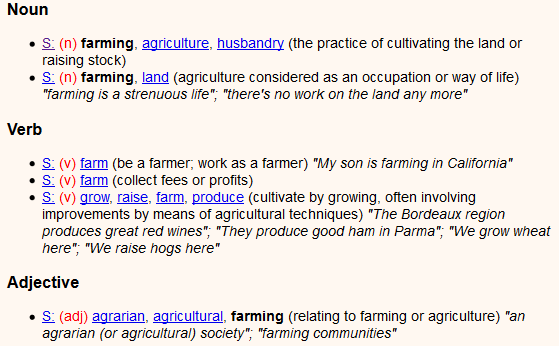
\includegraphics[width=\textwidth]{gfx/Wordnet/farming.png}
	\end{minipage}
	\begin{minipage}{0.5\textwidth}
		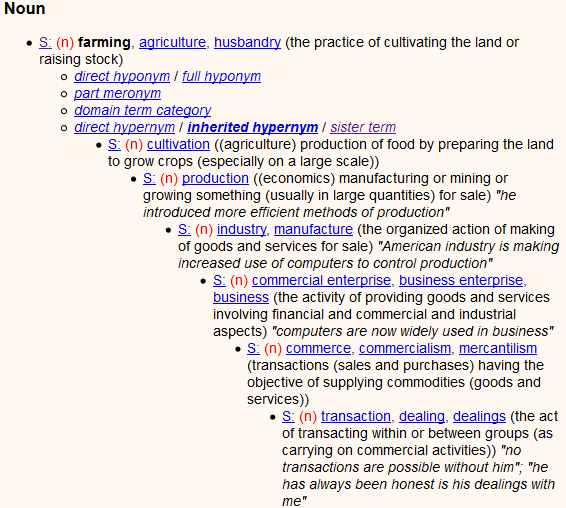
\includegraphics[width=\textwidth]{gfx/Wordnet/farmingTree.png}
	\end{minipage}
	\caption[WordNet results for the word \textit{farming}]{WordNet results for the word \textit{farming}. Adapted from \textit{WordNet}}
	\label{pic:Wordnet}
\end{figure}

To extract the information from WordNet we used the \textit{NLTK corpus reader}.\footnote{http://www.nltk.org/howto/wordnet.html} In addition to WordNet also Polyglot \footnote{https://polyglot.readthedocs.io/en/latest/Embeddings.html} was used as kind of preprocessing for selecting similar words of a topic by using word embeddings.
\subsubsection{Preprocessing}
For all following approaches in the next section we implemented a preprocessing step, that can be applied before running the different approaches for labeling a topic. It should improve the quality of the labels. 
Our topics consists of 10 words, usually these words can not be summarized to one label, which fits to all of the topic words. Therefore, the distances between every combination of two topic words were calculated with Polyglot embeddings. The top-5 words with the lowest distance between each other were selected. On these top words the labeling methods were applied.

\subsubsection{Finding labels with a scoring function}
Trying to find a good label for topics we used topic words \textit{w} and generated synsets \textit{s} for each topic word with the help of WordNet. Based on them we picked their direct hypernyms \textit{h}. To weight the hypernyms \ac{csf} was defined, which includes the number of hypernyms \textit{h} for the word \textit{w} and the number of words, that have a hypernym in common. When a hypernym for a word was found the reciprocal of the total number of hypernyms for each word was assigned to to every hypernym of the current word. If a selected hypernym is used by another word, too, the scores are added and then multiplied by the number of common words. We select the final label by the highest score.

Figure \ref{pic:HypFun} illustrates the scores for each hypernym, which are represented as circles above the hypernyms. The arrows connect the topic words \textit{w} with their synsets \textit{s}. These are connected to hypernyms \textit{h}. For $w_{1}$ each hypernym $h_{1},h_{2}$ has the value $\tfrac{1}{3}$. {$h_{4}$ and $h_{5}$ have the value $\tfrac{1}{2}$, 
	but $h_{5}$ is connected to $s_{5}$ and $s_{6}$. Therefore, we add up $\tfrac{1}{2}$ from $w_{2}$ and $\tfrac{1}{3}$ from $w_{3}$ and multiply the result by 2. In total $h_{5}$ reaches the highest score of $\tfrac{5}{3}$ and is selected as the final label.

\begin{figure}
	\centering
	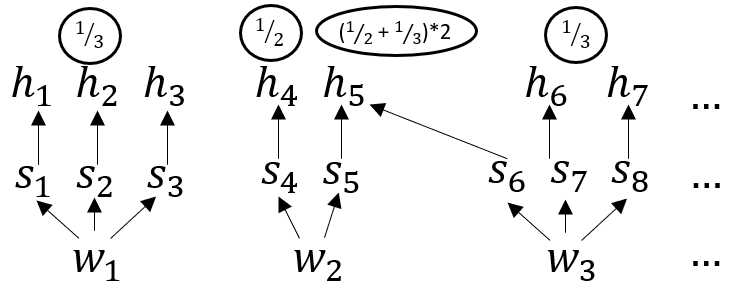
\includegraphics[width=0.5\textwidth]{gfx/Wordnet/HypFunF.png}
	\caption[\ac{ATL}: Scoring function for hypernyms]{Scoring function for hypernyms}
	\label{pic:HypFun}	
\end{figure}

\subsubsection{Find labels with similarity functions}
The first one utilizes similarity functions provided by WordNet. The second one relies on Polyglot word embeddings to calculate the distance between two terms.

WordNet offers different similarity functions, to calculate the similarity between synsets:
\begin{itemize}
\item The \textit{path-similarity} is defined by the nodes, which are visited while going from one word to another using the hypernym hierarchy. The distance between two words is the number of nodes that lie on the shortest path between two words in the hierarchy. The calculated score is in range of 0 and 1, while 1 means two words are identical.
\item The \textit{lch-similarity} (Leacock-Chodorow) is based on the shortest path $p$ and the maximum depth $d$ of the hierarchy in which the words occur. The path length is scaled by the maximum depth: $-log(p/2d)$\newline
\end{itemize}
The remaining three similarity functions are measuring the \ac{IC} of synsets. \ac{IC} combines the knowledge of the hierarchical structure from WordNet, with statistics on actual usage in text as derived from a large corpus. Per default WordNet uses the Brown Corpus. Although, this corpus is not related to our domain-specific data, it includes a large number of English texts and is suitable as a reference corpus for this specific task. 

\begin{itemize}
\item The \textit{res-similarity} (Resnik-Similarity) weights edges between nodes by their frequency of the used textual corpus. Based on the \ac{IC} of the Least Common Subsumer (lsc), the most specific ancestor node, a similarity score is calculated.
\item The \textit{jcn-similarity}(Jiang-Conrath Similarity) calculates the relationship between two words with $(IC(w_{1}) + IC(w_{2}) - 2 * IC(lcs))$ and \item the \textit{lin-similarity} calculates it with $2 * IC(lcs) / (IC(w_{1}) + IC(w_{2}))$.
\end{itemize}
%path sim better then ich because the labels were more specific.
% bsp mit tabelle, wie oft entity, abstraction, physical entity,physical object,whole
%und beispiel mit 3topics, dass die labels besser sind

For all topic words we generated synsets and calculated for all possible combinations of the topic words the similarities of their synsets. For every possible topic word pair the highest similarity score from the synsets was taken and the lowest common hypernym was derived. If a combination of topic words had the same lowest common hypernym, the similarities were summed up. In the end, the hypernym with the highest score was taken as the final label. 

The same procedure was applied also with Polyglot embeddings (plg). Instead of calculating the similarity between the synsets with WordNet similarity functions, the distance function from the Polyglot library was used. The lower the distance between two words the more similar they are. The other steps remained the same.

\subsection{Evaluation}
In the following section the results of intrinsic and extrinsic topic labeling will be evaluated regarding their quality and the number of different labels in a topic model. The labels generated automatically, are also compared to the manual labels, which were assigned by the domain experts. For the evaluation we used English editorial articles. First, we evaluate the intrinsic and second, the extrinsic topic labeling. Afterwards, the intrinsic and extrinsic labellings are compared with each other. 

\subsubsection{Intrinsic topic labeling}
\label{eval:intrinsic}
We applied the \ac{ATL} in section \ref{sec:intrinsic} on our datasets, which include editorials, comments and forums. In general, the \ac{ATL} according to \cite{Mei2007}, outputs only different labels for topics, which were generated with \ac{LDA}. For the topics generated with \ac{NMF} the same label was given for every topic in a topic model. The reason could be, that \ac{NMF} does not return a probability distribution for every document. Normalizing the values between 0 and 1 did not lead to an improvement. Therefore, the labels for topics generated with \ac{NMF} were neglected. Further evaluations are based on English editorial articles. 
\paragraph{Topics from Generation 1}
First, we used the topics from \textit{Generation 1}, which were generated as described in \ref{data:preprocessing}. In Figure \ref{fig:labelcount_intrinsic} the label counts for English editorial articles are shown. On the x-axis all labels are listen, while the y-axis denotes the number of topics, that the label was assigned to. 
Considering just  the labels without verifying the topics, they are assigned to, the labels seem to be meaningfull and specific. Often, a label is a persons name e.g {\textit{Jose Andres, Rahm Emanuel, Morgan Stanly,Gloria Casas, Theresa Eisemann etc.}}.
%mai with2bigrams
\begin{figure}[h]
	\centering
	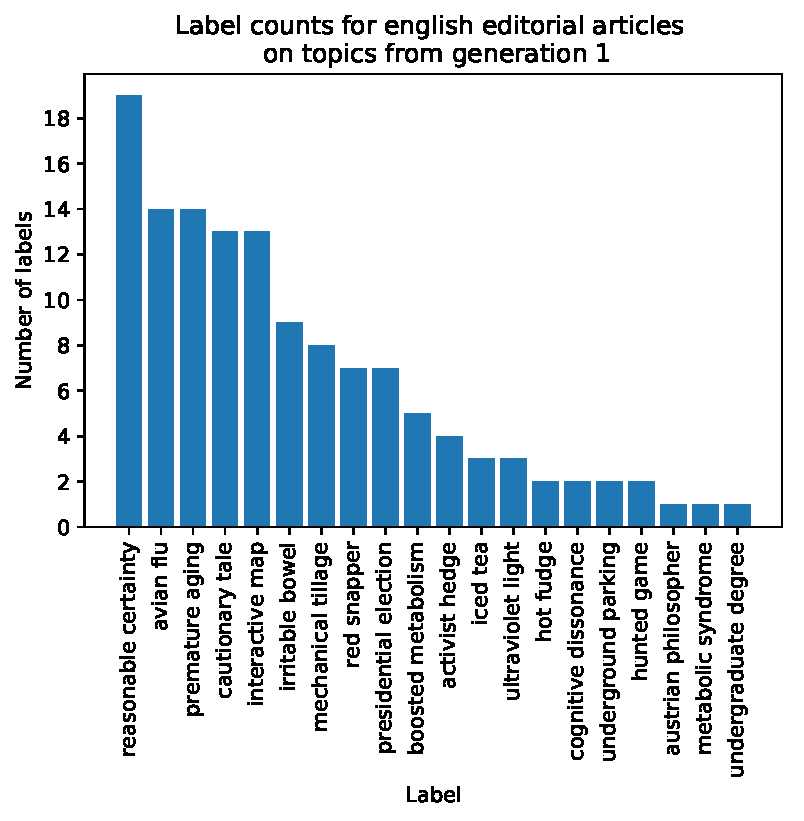
\includegraphics[width=7cm,height=7.5cm]{gfx/POS-gen1/alte_topics.pdf}
	\caption[Label counts for topics from Generation 1 with intrinsic labeling]{Label counts for topics from Generation 1 according to \cite{Mei2007}.}
	\label{fig:labelcount_intrinsic}
\end{figure}

In Table \ref{tab:extrinsic_manually} example topics are shown, which were labeled manually by domain experts and with the intrinsic approach. The intrinsic labels do not fit to the given topic: \textit{Rahm Emanuel} an American politician is assigned to Topic 107, which deals with environment and waste. \textit{Hairy vetch}, a plant variety, for Topic 23. \textit{Irritable bowel syndrome}  to Topic 64 and \textit{Safran Foer}, an American novelist, to Topic 74, dealing with animal husbandry. The automatic labels have nothing in common with the manual ones.
% mai label und hannah
%%tabelle mit hannas
\begin{table}[h]
	\begin{minipage}[t]{0.5\textwidth}
		\begin{tabular}{c|l}
			&Topic 107 \\
			\hline
			method & \thead{waste, compost, use, scrap, material,\\landfill, ton, environmental, throw, gas} \\
			\hline
			intrinsic & rahm emanuel  \\
			manual &waste	\\
			&\\
			%{topic 107}
		\end{tabular}
	\end{minipage}
	\begin{minipage}[t]{0.5\textwidth}
		\begin{tabular}{c|l}
			&Topic 23 \\
			\hline
			&\thead{grow, garden, plant, farm, vegetable, \\seed, year, tomato, produce, farming} \\
			\hline
			&hairy vetch\\
			&homegrown food	\\
			\\
			%{topic 23}
		\end{tabular}
	\end{minipage}
	\begin{minipage}[t]{0.5\textwidth}
		\begin{tabular}{c|l}
			&Topic 64\\
			\hline
			method& {\thead{milk, raw, dairy, product, cheese,claim,\\ health, cow drink, study }} \\
			\hline
			intrinsic &irritable bowel syndrome\\
			manual&dairy product\\
		\end{tabular}
	\end{minipage}
	%{topic 64}
	\begin{minipage}[t]{0.5\textwidth}
		\begin{tabular}{c|l}
			&Topic 74 \\
			\hline
			&\thead{meat, feed, beef, animal, grass,\\cow, eat, raise, buy, make} \\
			\hline
			&safran foer\\
			&animal husbandry	\\
		\end{tabular}
	\end{minipage}
	%{topic 74}
	\caption[Labeled topics manually and with intrinsic method and ]{Topics labeled manually and with intrinsic methods.}
	\label{tab:extrinsic_manually}
\end{table}

\paragraph{Topics including POS-tagging:}

By providing \ac{POS}-tags, using Spacy\footnote{Possible POS-tags: https://spacy.io/api/annotation}, we can limit the labels to certain word types. In our experiments we used (NN-NN) or (JJ-NN) \ac{POS}-tags for English topic labels and (NN-NN) or (ADJD-NN) for German.  To apply \ac{POS}-tagging, the preprocessing for the texts had to be changed, because in Generation 1, a collocation finder was used. After performing this step the \ac{POS}-tags could not be applied retroactively. Therefore, we removed collocation finding and added \ac{POS}-tagging. All other preprocessing steps remained the same. Nevertheless, the topics differ from the ones of Generation 1. 

In Table \ref{tab:intrinsic_label_pos} topics and labels are shown with different \ac{POS}-tags. In comparison to the labels generated without \ac{POS}-tagging, these labels seem closer to a topic. For Topic 6, 10, 23 and 37 the labels \textit{music festival, premature aging, hunted games} and \textit{modified organism} seem good.

%with pos and without
\begin{table}[h]
	\begin{minipage}[t]{0.5\textwidth}
		\begin{tabular}{c|c}
			&Topic 6\\
			\hline
			with \ac{POS}-tags & \thead{restaurant, fast, chain, meal,\\ say, menu, ingredient,\\ burger, chipotle, mcdonald } \\
			\hline
			(NN, NN) & music festival   \\
			(JJ, NN) & hot fudge \\
			-  & dunkin donuts\\
			&\\
		\end{tabular}
		%{topic 6}
	\end{minipage}
	\begin{minipage}[t]{0.5\textwidth}
		\begin{tabular}{c|c}
			&Topic 10\\
			\hline
			& \thead{child, eat, kid,\\ parent, family,	healthy,\\ school, who, 	health,can } \\
			\hline
			& anorexia nervosa \\
			& premature aging   \\
			& anorexia nervosa	\\
			&\\
		\end{tabular}
		%{topic 10}
	\end{minipage}
	\begin{minipage}[t]{0.5\textwidth}
		\begin{tabular}{c|c}
			&Topic 23\\
			\hline
			with \ac{POS}-tags &  \thead{meat, beef, feed,animal, grass,\\ cattle,eat,\\ raise, more, pork} \\
			\hline
			(NN, NN) & sport utility \\
			(JJ, NN) & hunted game   \\
			-& earl butz	\\
		\end{tabular}
	\end{minipage}
	\hfill\hfill
	%{topic 23}
	\begin{minipage}[t]{0.5\textwidth}
		\begin{tabular}{c|c}
			&Topic 37\\
			\hline

			& \thead{carbon, climate, gas,\\ 	greenhouse, emission, change,\\ 	reduce, 	global, 	industrial, 	co2} \\
			\hline
			& gene splicing  \\
			& interactive map   \\
			& modified organisms\\
		\end{tabular}
	\end{minipage}
	%{topic 37}
	\caption[Labeled topics according with intrinsic method]{Labeled topics with intrinsic method}
	\label{tab:intrinsic_label_pos}
\end{table}

In Figure \ref{fig:labelcount_intrinsic_pos} the label counts for English editorial articles using the texts, that were \ac{POS}-tagged are shown. On the x-axis all labels are listed, while the y-axis denotes the number of same labels. 
In the plots where \ac{POS}-tags were applied, no labels include a name of persons and a smaller number of labels was outputted in contrast to the plot without \ac{POS}-tags. 

However, the same observation can be made as above. Although, the labels seem meaningful and specific they do not really fit to the topics. We assume that the high quality of the labels themselves stem from the way they are generated. By applying bi-gram mining on the original corpus only useful word combinations are found as candidate labels. That the labels seemingly do not fit to the topics means that measuring the relatedness between the topics and the labels by their KL-divergence is not successful on our data.

%label counts for pos
\begin{figure}[h]
	\begin{minipage}[t]{0.5\textwidth}
		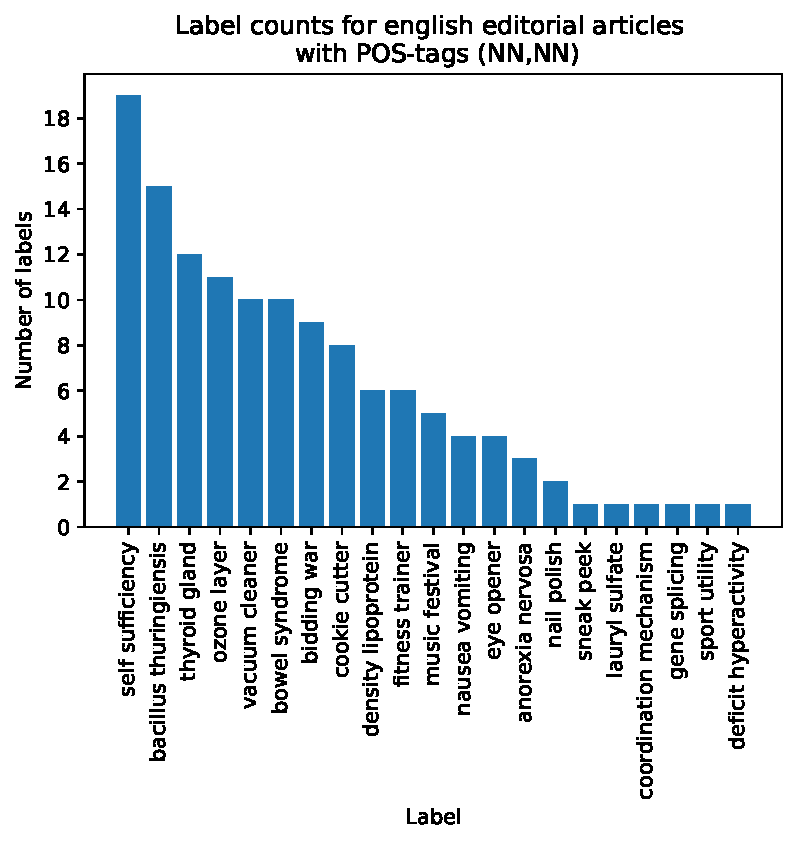
\includegraphics[width=7cm,height=7.5cm]{gfx/POS-gen1/mit_NN.pdf}
	\end{minipage}
	\begin{minipage}[t]{0.5\textwidth}
		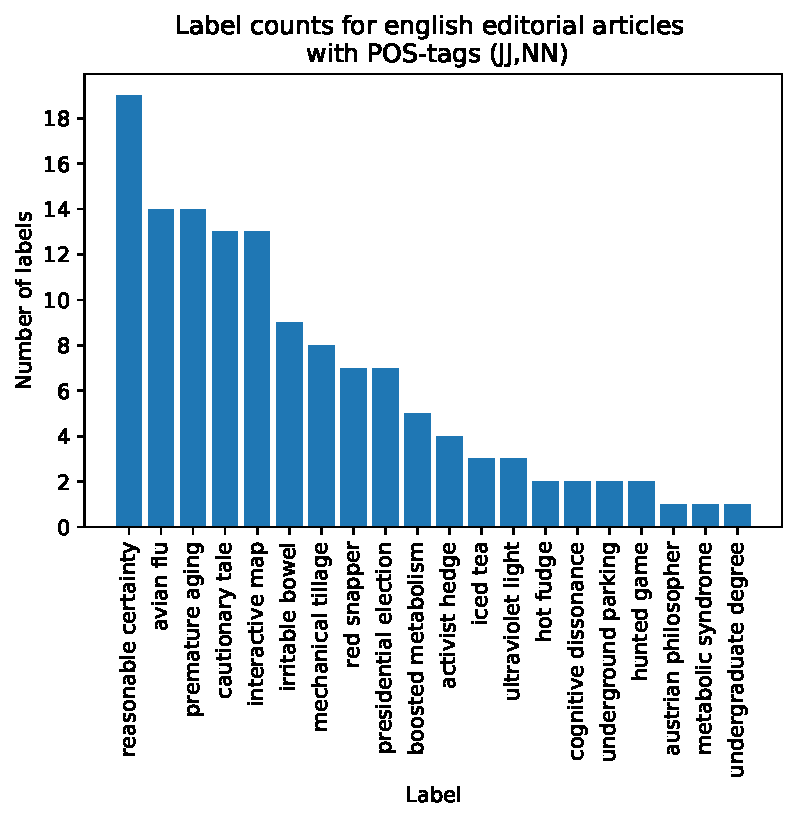
\includegraphics[width=7cm,height=7.5cm]{gfx/POS-gen1/mit_JJNN.pdf}
	\end{minipage}
	\begin{minipage}[t]{0.5\textwidth}
		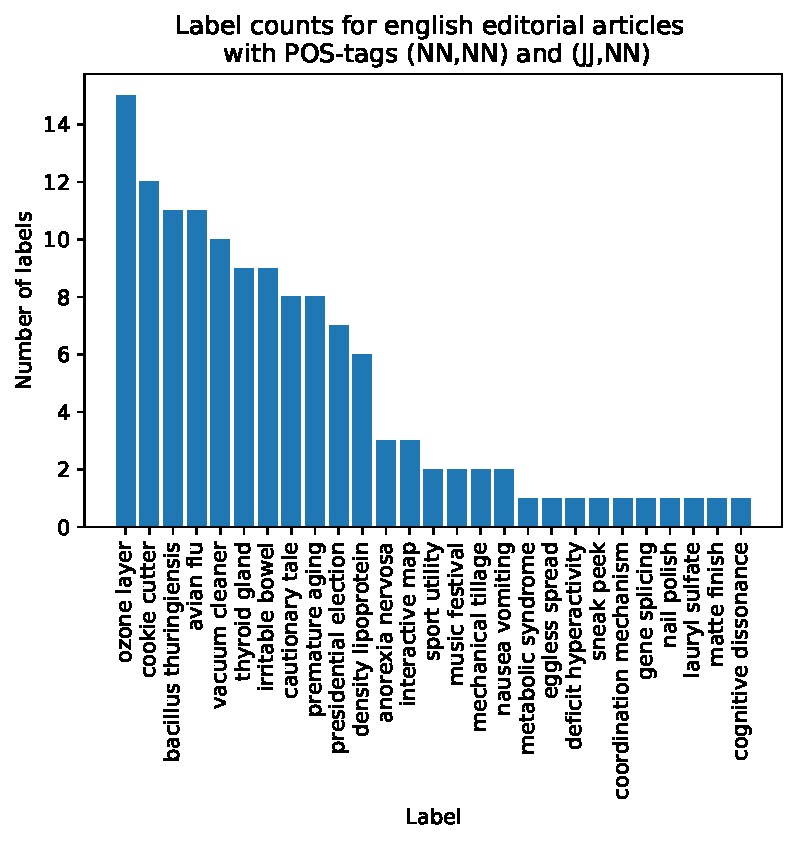
\includegraphics[width=7cm,height=7.5cm]{gfx/POS-gen1/mit_beiden_pos.pdf}
	\end{minipage}
	\begin{minipage}[t]{0.5\textwidth}
		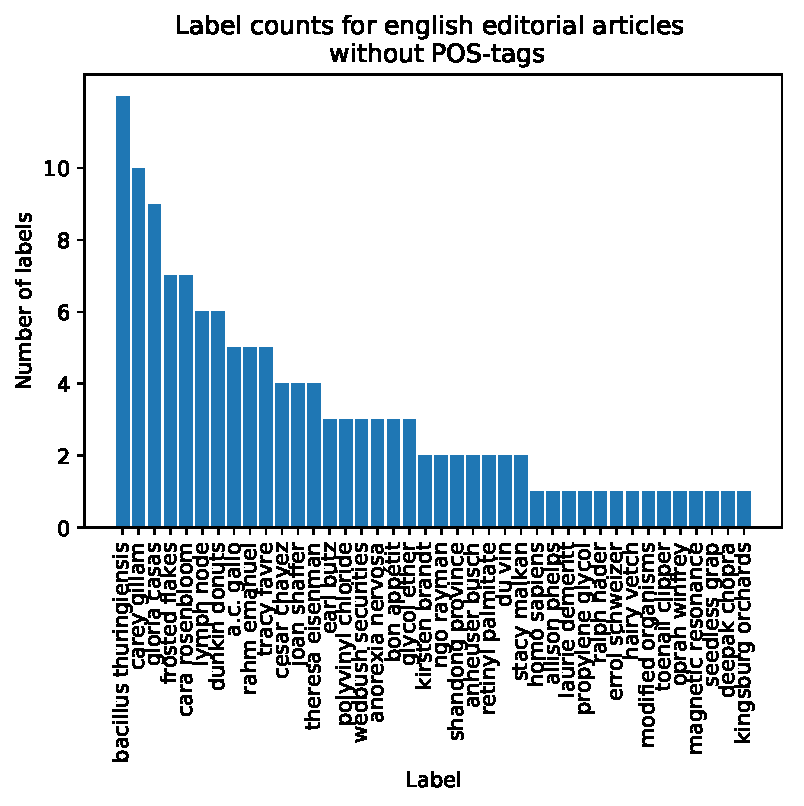
\includegraphics[width=7cm,height=7.5cm]{gfx/POS-gen1/ohne_POS.pdf}
	\end{minipage}
	\caption{Label counts for topics including \ac{POS}-tags with intrinsic method.}
	\label{fig:labelcount_intrinsic_pos}
\end{figure}

\subsubsection{Extrinsic topic labeling}
\label{eval:extrinsic}
Furthermore, we applied the \ac{ATL} in section \ref{sec:extrinsic} on our Dataset, using the English online database WordNet and Polyglot embeddings. The described different similarity functions from WordNet, the \ac{csf} and the Polyglot embeddings were used to label our topics. A few examples are shown in Table \ref{tab:labeled_extrinsic_and_manually} including the manual assigned labels to the topics, too. Some labels generated with the automatic approaches match the manual assigned labels. This is the case for the Topics 64, 84 and 107. For the other topics, the labels are heading to the same direction as the manual label: for Topic 97 \textit{chemical} and manually \textit{pesticide residues}, for Topic 99 \textit{bee} and manually \textit{beekeeping} and for Topic 109 \textit{grocery store, mercantile establishment, marketplace} and manually \textit{retailers} were assigned.
%%tabelle mit hannas
\begin{table}
	\begin{minipage}[t]{0.5\textwidth}
		\begin{tabular}{c|ll}
			&Topic 23 &\\
			\hline
			method&\multicolumn{2}{l} {\thead{grow, garden, plant, farm, vegetable, \\seed, year, tomato, produce, farming}} \\
			\hline
			path&entity 	& produce  \\
			ich&entity	& produce\\
			res&produce		& produce\\
			jsn&produce	& produce\\
			lin&produce		& produce\\
			plg&vegetable	& vegetable\\
			\ac{csf}&cultivate  & cultivate\\
			manual&\multicolumn{2}{l}{homegrown food}	\\
			&\\
			%{topic 23}	
		\end{tabular}
	\end{minipage}
	\begin{minipage}[t]{0.5\textwidth}
		\begin{tabular}{c|ll}
			&Topic 64 &\\
			\hline
			& \multicolumn{2}{l} {\thead{milk, raw, dairy, product, cheese,  cow\\health, drink, study, claim }} \\
			\hline
			& abstraction 	& beverage  \\
			& abstraction	& produce\\
			& \textbf{dairy product}		& beverage\\
			& produce	& beverage\\
			& beverage		& beverage\\
			& \textbf{dairy product}	& abstraction\\
			& nakedness  & farm\\
			& \multicolumn{2}{l}{\textbf{dairy product}}	\\
			&&\\
			%topic 64
		\end{tabular}
	\end{minipage}
	\begin{minipage}[t]{0.5\textwidth}
		\begin{tabular}{c|ll}
			&Topic 74 &\\
			\hline
			method&\multicolumn{2}{l} {\thead{meat, feed, beef, \\ grass, eat, raise, cow, buy, make, animal}} \\
			\hline
			path&entity 	& meat  \\
			ich&entity	& abstraction\\
			res&matter		& meat\\
			jsn&food	& meat\\
			lin&matter		& meat\\
			plg&cattle	& physical entity\\
			\ac{csf}&cattle  & be\\
			manual&\multicolumn{2}{l}{animal husbandry}	\\
			&&\\
			% {topic74}
		\end{tabular}
	\end{minipage}
	\begin{minipage}[t]{0.5\textwidth}
		\begin{tabular}{c|ll}
			&Topic 84 &\\
			\hline
			& \multicolumn{2}{l} {\thead{company, tea, brand, product, drink, \\honest, new, beverage, consumer, 	goldman}} \\
			\hline
			& \textbf{beverage}  & \textbf{beverage}\\
			& physical entity	& substance\\
			& substance	& substance\\
			& \textbf{beverage}		& \textbf{beverage}\\
			& \textbf{beverage}	& \textbf{beverage}\\
			& food 	& food  \\
			& \textbf{beverage}	& \textbf{beverage}\\
			& \multicolumn{2}{l}{\textbf{beverage}}	\\
			&&\\
			%topic 84
		\end{tabular}
	\end{minipage}
	\begin{minipage}[t]{0.5\textwidth}
		\begin{tabular}{c|ll}
			&Topic 97 &\\
			\hline
			method&\multicolumn{2}{l} {\thead{fruit, vegetable, pesticide, produce, buy, \\eat, list, apple, residue, sweet}} \\
			\hline
			path& matter& matter\\
			ich&matter	& matter\\
			res&matter	& matter\\
			jsn&matter	& matter\\
			lin&produce	& matter\\
			plg&fruit  & entity\\
			\ac{csf}&chemical 	& chemical\\
			manual&\multicolumn{2}{l}{pesticide residues}	\\
			&&\\
			%{topic 97}
		\end{tabular}
	\end{minipage}
	\begin{minipage}[t]{0.5\textwidth}
		\begin{tabular}{c|ll}
			&Topic 99 &\\
			\hline
			& \multicolumn{2}{l} {\thead{bee, honey, study, hive, year, \\beekeeper, plant, researcher, honeybee, colony}} \\
			\hline
			& organism & person  \\
			& organism	& person\\
			& organism	& organism\\
			& organism	& whole\\
			& bee	& artifact\\
			& bee	& artifact\\
			& farmer 	& scientist\\
			& \multicolumn{2}{l}{beekeeping}\\
			&&\\
			%topic 99
		\end{tabular}
	\end{minipage}
	\begin{minipage}[t]{0.5\textwidth}
		\begin{tabular}{c|ll}
			&Topic 107 &\\
			\hline
			method & \multicolumn{2}{l} {\thead{waste, compost, use, scrap, material, \\landfill, ton, environmental, throw, gas}} \\
			\hline
			path & material 	& material  \\
			ich  & abstraction	& physical entity\\
			res  & material		& material\\
			jsn  & abstraction	& material\\
			lin  & material		& material\\
			plg & \textbf{waste}	& abstraction\\
			\ac{csf} & convent  & lowland\\
			manual & \multicolumn{2}{l}{\textbf{waste}}	\\
		\end{tabular}
	\end{minipage}
	\begin{minipage}[t]{0.5\textwidth}
		\begin{tabular}{c|ll}
			&Topic 109 &\\
			\hline
			& \multicolumn{2}{l} {\thead{foods, company, store, chain, market,\\ executive, new, year, mackey,	grocery}} \\
			\hline
			& grocery store 	& mercantile establishment\\
			& physic entity	& mercantile establishment\\
			& social group	& mercantile establishment\\
			& grocery store	& mercantile establishment\\
			& social group	& mercantile establishment\\
			& artifact	& abstraction\\
			& marketplace  & marketplace\\
			& \multicolumn{2}{l}{retailer}	\\
			%topic 84
		\end{tabular}
	\end{minipage}
	%{topic 74}
	\caption[Labeled topics with extrinsic methods and manually]{Topics labeled from Generation 1 manually and with extrinsic methods. Labels including preprocessing are in the third and fifth column. \textbf{Bold} words are the same as the manual assigned label.}
	\label{tab:labeled_extrinsic_and_manually}
\end{table}
Evaluating the automatically generated labels using different approaches, it was discovered that depending on the topics different labeling techniques output the best labels. It is not possible to tell, which approach is the best for all topics, let alone for several topic models according to the labels. Therefore, we tried to evaluate the labels generated with the extrinsic methods according to label counts. The words \textit{entity, physical entity, object, whole, matter} and \textit{abstraction} were chosen, because these are the most general words in the hierarchical tree of hypernyms in WordNet and do not have a high informative value. 
In Table \ref{tab:label_count_non_informative} the number of non informative words are listed for the different similarity functions from WordNet. Based on the sum of the non informative words per similarity function and Polyglot embeddings (plg), we ranked the different methods in Table \ref{tab:ranked_non_info}. The top 3 are: res-similarity with preprocessing, lin-similarity with preprocessing and Polyglot embeddings.
%%labelcount uninformative words
\begin{table}[h]
	\begin{tabular}{c|c|c|c|c|c|c|c}
		%& \multicolumn{6}{c}{Count of labels}\\
		%\hline
		method & entity	& physical entity & object & whole & matter & abstraction & $\sum$ \\
		\hline
		path& 19		&20				  &7	   &4      &1       &33 &84\\
		& \textbf{7}&\textbf{7}	 &\textbf{5}  &\textbf{2} &\textbf{1} &\textbf{16} & 38\\
		\hline
		ich& 29		&23				  &7	   &4      &1       &42 & 106\\
		& \textbf{13}&\textbf{13}	 &\textbf{9}  &\textbf{3} &\textbf{1} &\textbf{25} & 64\\
		\hline
		res& -		&4				  &5	   &4      &9       &5 &27\\
		& -			&\textbf{2}	 &\textbf{4}  &\textbf{1} &\textbf{2} &\textbf{1} &10\\
		\hline
		jsn& 19		&14				  &3	   &2      &1       &25 &64\\
		&10 		&\textbf{6}	 &\textbf{2}  &\textbf{2} &\textbf{2} &\textbf{9} &31\\
		\hline
		lin& -		&1				  &8	   &6      &9       &11 &35\\
		& -	 	&\textbf{1}	 &\textbf{3}  &\textbf{5} &\textbf{3} &\textbf{5} &17\\
		\hline
		plg& 1		&1		 &3	   &6      &4       &3 &18\\
		& \textbf{7}&\textbf{7}	 &\textbf{4}  &\textbf{7} &\textbf{3} &\textbf{19} & 47\\
	\end{tabular}
	\caption[Label counts of non informative words]{Label counts of non informative words with different similarity functions. \textbf{Bold} numbers denote labels including preprocessing.}
	\label{tab:label_count_non_informative}
	%fett sind die preprzesseten labels
\end{table}
\begin{table}[h]
	\begin{tabular}{|l|l|l|}
		\hline
		1. \textbf{res-similarity} &2. \textbf{lin-similarity} &
		3. polyglot embeddings (plg) \\ 
		\hline
		4. res-similarity&5. \textbf{jsn-similarity}& 6. lin-similarity\\
		\hline
		7. \textbf{path-similarity} &8. \textbf{polyglot embeddings} &9. jsn-similarity \\ 
		\hline
		10. \textbf{ich-similarity}&11. path-similarity  &12. ich-similarity\\
		\hline
	\end{tabular}
\caption[Ranked similarity functions for extrinsic labeling]{Ranked similarity functions. \textbf{Bold} similarities denote the similarities, which were applied on preprocessed topics.}
\label{tab:ranked_non_info}
\end{table}
The labels with \ac{csf} do not include any non informative words, because only the direct hypernyms and not the whole hierarchy of hypernyms were considered. Therefore, we plotted the amount of distinct labels in Figure \ref{extr_csf_count}. This shows, the labels generated with preprocessing on the left side and the labels without on the right. The number of same labels is at most 6 or 8, which shows that the labels are discriminative.
\begin{figure}
	\begin{minipage}{0.5\textwidth}
		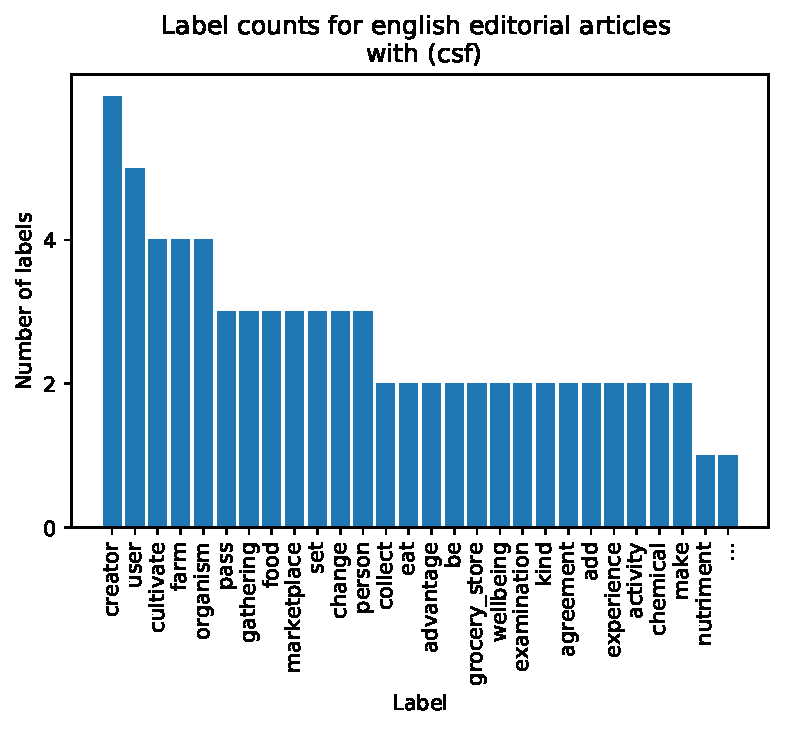
\includegraphics[width=7cm,height=7.5cm]{gfx/ATL_sim/with_scoring_pre.pdf}
	\end{minipage}
	\begin{minipage}{0.5\textwidth}
		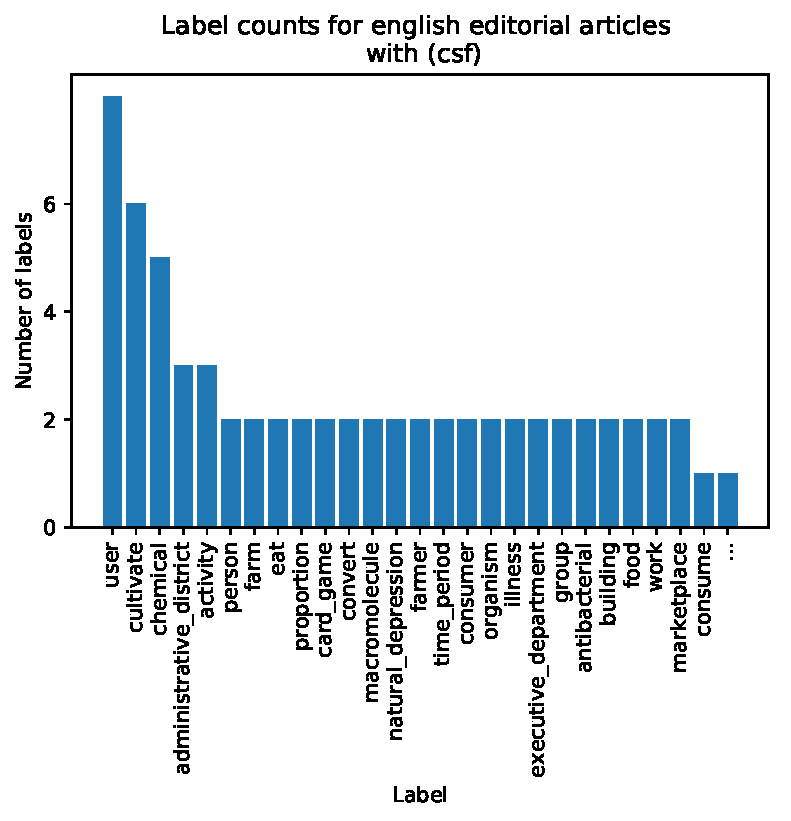
\includegraphics[width=7cm,height=7.5cm]{gfx/ATL_sim/with_scoring.pdf}
	\end{minipage}
	\caption{Label counts for topics from Generation 1 with \ac{csf}.}
	\label{extr_csf_count}
\end{figure}

Having evaluated the intrinsic and extrinsic automatic topic labeling we can conclude, that the intrinsic approach generates meaningful and specific labels, that do not fit to the topics. The extrinsic approach  generates partially good results, which are comparable with the labels from the domain experts. Nevertheless, finding meaningful and high qualitative labels is not yet automatable. The knowledge and experience a human person, which is required for topic labeling, can not be replaced by a machine.

\cleardoublepage


\newpage
\section{Internal consistency}
\label{Internal_consistency}
When generating a topic model with \ac{LDA} or \ac{NMF} the number of topics has to be manually set. This number is critical and has an effect on the quality and the interpretability of topics. We want to provide the domain experts an overview how topics change when increasing or decreasing the topic number. So they can assess, which topic model is the appropriate one for their further research. 

To analyze the quality of a topic model we differentiate between the intra topic model and inter topic model approach. The intra topic approach compares all topics of one topic model with each other. This way we can study, which topics are similar to each other or which topics appear together in the same document. When applying the inter topic approach, we compare the topics from topic model A to a second different topic model B. The second topic model differs from the first by the number of topics. By comparing the two models we can study what effect the increasing topic number has on the quality of the topics. With both approaches we want to examine questions such as: Do the topics get more specific, more general, do they split up or do they stay the same and only new topics are added? Are there a few topics, which are dominating in a document or are few topics assigned to a document? How does the topic assignment change across different topic models? Indicates a higher topic number a better clustering of the documents?

Both, \ac{LDA} and \ac{NMF} return a document topic matrix $\theta$, which describes to what extend a topic appears in a document and a topic term matrix $\phi$, which describes to what extend a term appears in a topic. Different key figures can be derived from these matrices to judge the quality and to examine the changes in topics.
Entropy and Jensen Shannon divergence can be used on the document topic matrix as well on the topic term matrix. The coherence measure relies solely on the topic term matrix and alpha $\alpha$  can only be applied on topic models, that were generated with \ac{LDA}.

For our evaluation we generated topic models with 25, 50, 75 topics and topic models with 50 topics over and under the topics number from \textit{Generation 1}. The different key figures were applied on these newly generated topic models and the topic models from \textit{Generation 1}.In the following the dataset for \text{German editorial articles} with 25, 50, 75, 140, 190 and 240 topics per topic model were analyzed.

\subsection{Theta $\theta$}
\begin{table}[h]
	\centering
	\begin{tabular}{c|ccccc}
		&Topic 1&Topic 2&Topic 3&Topic 4&Topic 5\\
		\hline
		Document 1&0.1 & 0.4 & 0.05 & 0.25 & 0.2  \\
		Document 2&0.025&0.8 & 0.025 & 0.07 & 0.03\\
	\end{tabular}
	\caption[Document topic matrix]{Example for a document topic matrix}
	\label{doc_topic}
\end{table}
The document topic matrix $\theta$ describes to which extend a topic is represented in a certain document.
We used the matrix to calculate the number of documents, which are assigned to a topic and the number of topics, which are assigned to a document. In both cases a threshold fo 10\% was used. The example document topic matrix in Table \ref{doc_topic} shows two documents and 5 topics. For topic 1 the counter number of documents is only 1 (Document 1). For Document 1 the relevant number of topics is 4 (Topic 1,2,4,5). 

\subsection{Alpha}
Alpha $\alpha$ is a prior parameter for \ac{LDA}, that describes the sparsity of the topic distribution for every document. Usually, the prior $\alpha$ has to be set and has the same value for every topic. In this case it is called the symmetric Dirichlet prior. However, \cite{Blei2003} showed how $\alpha$ can be estimated from the data per topic. In this case $\alpha$ is an asymmetric Dirichlet prior. This method was used for our topic model, to determine how important the topics are for the whole corpus. A high $\alpha$ value means that the documents are mixtures of many topics, while a low $\alpha$ value means, that the documents are composed of only a few highly probable topics (\cite{Steyvers2007}).

In Figure \ref{alpha_dist} the alpha values for each topic for German editorial articles with 190 topics are shown. The document distribution for Topic 30, which has the lowest alpha value, is considered in Figure \ref{alpha_min}. The x-axis represents the document ids, standing for the documents, which build the corpus. The y-axis represents the percentage of a document that is covered by the topic. In contrast to Topic 30, Topic 111 with the highest alpha value is shown in Figure \ref{alpha_max}. One can see, that Topic 30 covers only a few documents, while Topic 111 is more evenly spread over all documents.

%%beispiel für alpha
\begin{figure}[h]
	\centering
	\subfloat[Plotted alphas for German editorial articles]{\label{alpha_dist}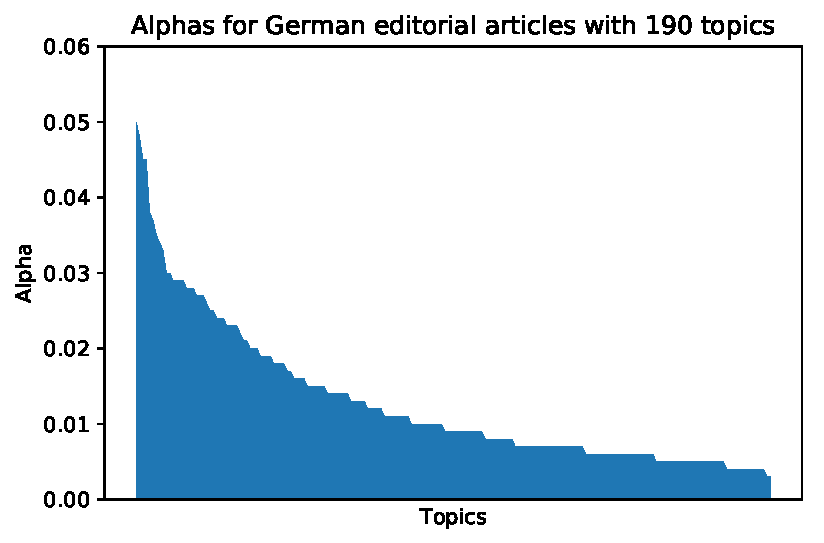
\includegraphics[width=8cm]{gfx/Alphas/German_editorial_articles_with_190_topics_100.pdf}}\par\medskip
	\begin{minipage}{0.5\textwidth}
		\centering
		\subfloat[Document coverage for the topic with the lowest alpha value ]{\label{alpha_min}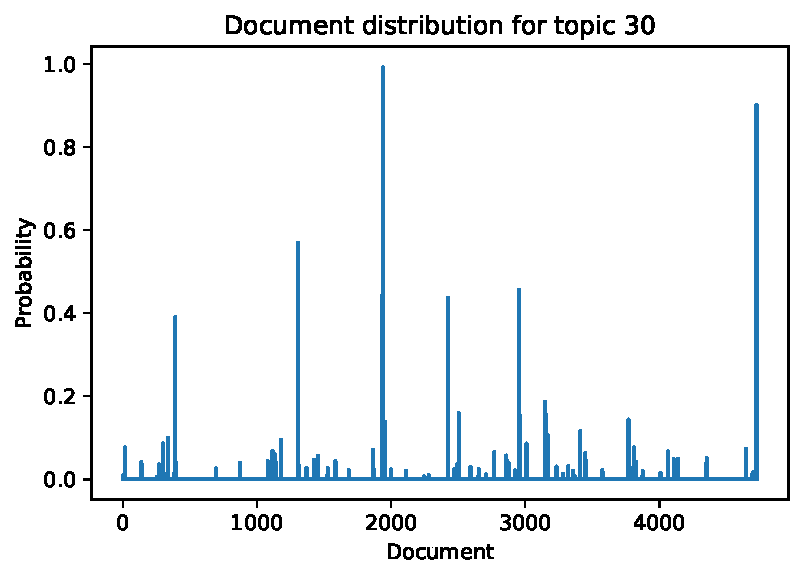
\includegraphics[width=7cm]{gfx/doc_topic_max_min/German190t30.pdf}}
	\end{minipage}%
	\begin{minipage}{0.5\textwidth}
		\centering
		\subfloat[Document coverage for the topic with the highest alpha value]{\label{alpha_max}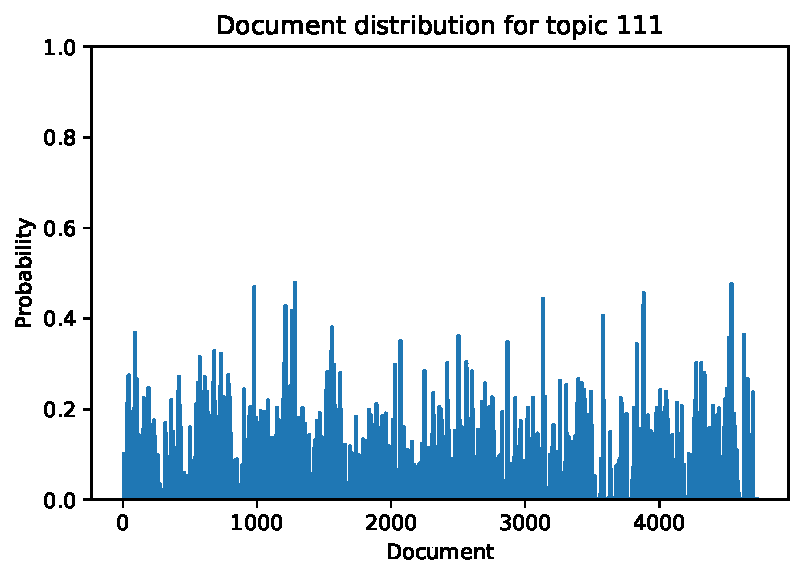
\includegraphics[width=7cm]{gfx/doc_topic_max_min/German190t111.pdf}}
	\end{minipage}
	\caption[]{Alpha values for German editorial articles with 190 topics and the topic document matrices for the topic with the highest and lowest alpha value}
	\label{alpha_example}
\end{figure}

\newpage
\subsection{Entropy}
Entropy was used to identify specific and general topics. It can be applied on the topic term matrix $\phi$ and the document topic matrix $\theta$. When applied on the topic term matrix, a high entropy value indicates that the topic is rather general. This means, that all terms have a similar probability to appear in the topic. A low entropy indicates, that the topic is specific i.r. only a few words have a high probability to appear in the topic. This difference is illustrated in Figure  \ref{entropy_min} and in Figure \ref{entropy_max}. \newline
When applied on the document topic matrix $\theta$ the rules can be applied analogously. A high entropy value indicates, that the topic is rather general. This means, that all topics have a similar probability to appear in a document. A low entropy value indicates, that the topic is specific i.e. only a few topics have a high probability to appear in a document. Entropy is calculated as follows (\cite{Sethi2012}):
\begin{equation}
E = -\sum(p * log(p))
\end{equation}
where $p$ is the probability of a term in a topic, which was taken from the topic term matrix $\phi$ or the probability of a topic in a document, taken from the document topic matrix $\theta$. 
In Figure \ref{entropy_dist} the entropy values for each topic for German editorial articles with 190 topics are shown. The entropy values are sorted descending. The topic term matrix for Topic 13, which has the lowest entropy value, is considered in Figure \ref{entropy_min}. The x-axis represents each termid of the corpus. The y-axis represents the probability of the terms in a topic. In contrast to Topic 13, Topic 100 with the highest entropy value is shown in Figure \ref{entropy_max}. One can see, that Topic 13 consists mainly of the term id 4916 and the other term ids hardly occur, while in Topic 100 the term ids are nearly evenly spread.
\begin{figure}[h]
	\centering
	\subfloat[Plotted entropy for German editorial articles]{\label{entropy_dist}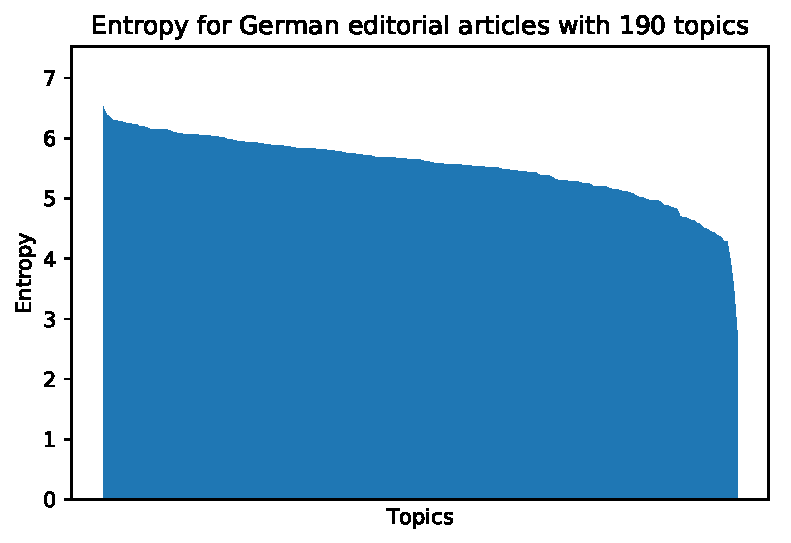
\includegraphics[width=7cm]{gfx/Entropy/German_editorial_articles_with_190_topics100.pdf}}\par\medskip
	\begin{minipage}{0.5\textwidth}
		\centering
		\subfloat[Topic coverage for the topic with the lowest enropy ]{\label{entropy_min}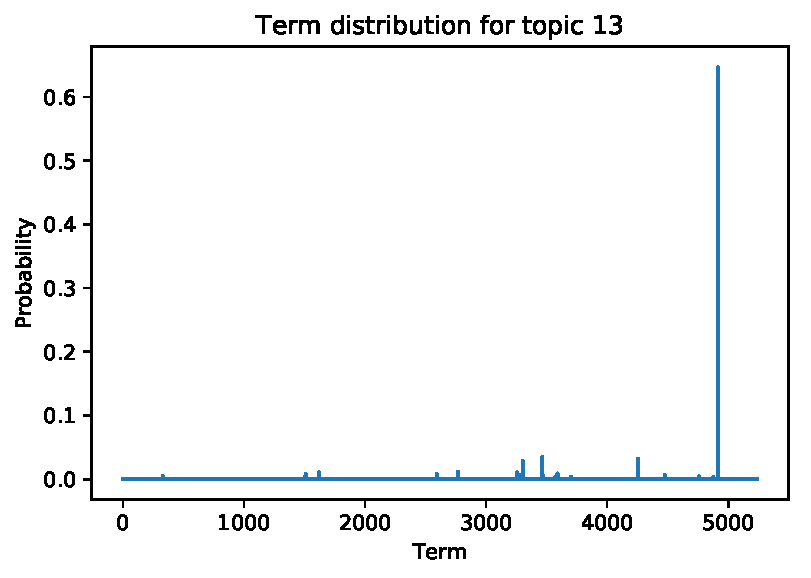
\includegraphics[width=6.65cm]{gfx/topic_term_max_min/German190t13.pdf}}
	\end{minipage}%
	\begin{minipage}{0.5\textwidth}
		\centering
		\subfloat[Topic coverage for the topic with the highest entropy ]{\label{entropy_max}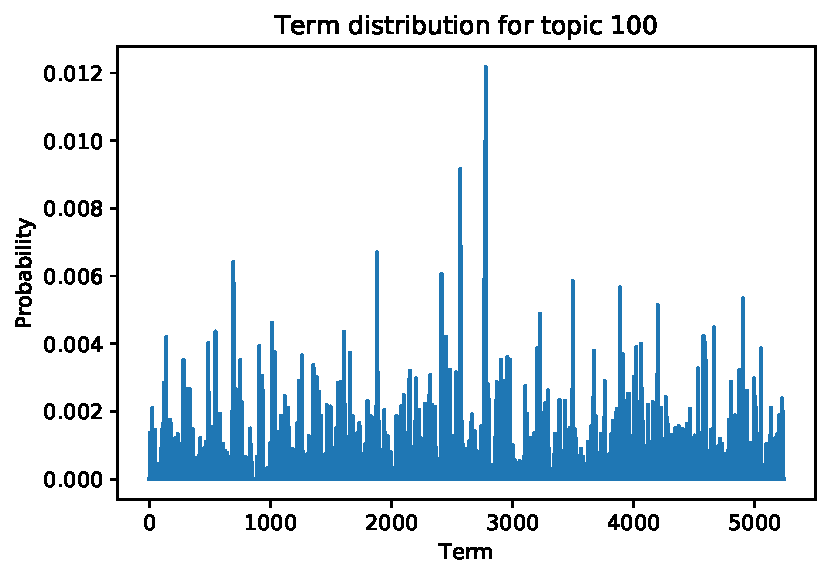
\includegraphics[width=7cm]{gfx/topic_term_max_min/German190t100.pdf}}
	\end{minipage}
	\caption[]{Entropy for German editorial articles with 190 topics and the topic term matrices for the topic with the highest and lowest entropy}
	\label{entropy_example}
\end{figure}


\subsection{Coherence}
The coherence scores topics by measuring the degree of semantic similarity between words in a topic. This measurement helps to distinguish topics, that are semantically similar and easy interpretable for humans and those that are semantically dissimilar and not easy interpretable.(\cite{Stevens2012}) There are different coherence measure such as the UCI-measure (\cite{Newman2010}) and the U-mass measure(\cite{Mimno2011}). Both measure the coherence of a topic as the sum of pairwise distributional similarity scores over a set of topic words:
%Both measures compute the coherence of a topicas the sum of pairwise distributional similarity scores over the set of topic words, V .
\begin{equation}
coherence (V) = \sum_{v_{i},v_{j}\in V} score(v_{i},v_{j})
\end{equation}
$V$ describes the set of words for a topic, while $v$ is a single word, occurring in a topic. We used the top-10 words of a topic to calculate the coherence score for each topic in a topic model.
We used the UMass metric, which is based on the document co-occurrence and defined as: 
\begin{equation}
socre(v_{i},v_{j}) = log\frac{D(v_{i},v_{j})+1}{D(v_{j})}
\end{equation}
$D(v_{j})$ is the document frequency, that count the number of documents which include the word $v_{j}$. $D(v_{i},v_{j})$ is the co-document frequency, that counts the documents, which include both word $v_{i}$ and $v_{j}$. A smoothing count of 1 is included to avoid taking the logarithm of zero. The UMass metric computes these counts over the original corpus, which was used to train the topic models (\cite{Stevens2012}). The coherence score is negative and the higher interpretability of a topic is given with a score near to zero.

\subsection{Jensen Shannon divergence}
The topics returned by \ac{LDA} are probability distributions over all terms in the corpus. Therefore, to compare the similarity of two topics $p$ and $q$ we can use existing metrics to measure the similarity between probability distribution. \cite{Lin1991} et al lists possible similarity functions. A standard function to measure the difference or divergence between two probability distributions $p$ and $q$ is the Kullback Leibler (\ac{KL}) divergence:
\begin{equation}
	D(p,q) = \sum_{j=1}^{T} p_{j} log_{2} \frac{p_{j}}{q_{j}}
\end{equation}
 where $j$ is the number of a certain term and $T$ describes the total number of terms. $p_{j}$ represents the probability of term $j$ appearing in topic $p$. $q_{j}$ is the probability of term $j$ appearing in topic $q$. The \ac{KL} divergence is an asymmetric measurement. For our use-case, comparing the topics intra and inter a topic model, a symmetric measure is needed, which guarantees the same results for the comparison of $t1$ with $t2$ and $t2$ with $t1$. Therefore, based on the \ac{KL} divergence, the \ac{JS} divergence is used:
\begin{equation}
	JS(p,q)  = 0.5 * (D(p,\frac{p + q}{2}) + D(q, \frac{p + q}{2}) )
\end{equation}
The \ac{JS} divergence  is a symmetric extension of the \ac{KL} divergence. If the probability distributions are identical, the value 0 is assigned otherwise the value 1 is assigned for totally dissimilar probability distributions (\cite{Steyvers2007}).
In our implementation we subtracted the value from the \ac{JS} divergence from 1 to get the similarity between two probability distributions, so that the value 1 is assigned when two probability distributions are identical and the value 0 when they are completely dissimilar. 

\subsection{Evaluation}
The evaluation was conducted on \textit{German} and \textit{English editorial articles}. For both datasets we studied topic model with 50 topics over and under the optimal topic number from \textit{Generation 1} and further generated topic models with 25, 50 and  75 topics. Both datasets were analyzed by applying each key figure as explained above on each topic model. The results per key figure and per topic model were then compared with each other.

\subsubsection{Entropy}

The Figures \ref{entr_german} and \ref{entr_english} show the change of entropy for \textit{German} respectively \textit{English editorial articles}. The table on the left denotes the minimal and maximal entropy given the number of topics. On the right the maximal entropy values (blue line) and the minimal entropy values (orange line) are plotted. This structure will repeat in the different key figures.

The entropy values for \textit{German editorial articles} (Figure \ref{entr_german}) are decreasing when increasing the number of topics. For the topic model with 240 topics the entropy values starts increasing again. This means, that the topics with a higher topic number are getting more specific until a certain point, when the entropy value is increasing again. This could mean, that the optimal topic number, to generate topics, which are specific, is at the point, when the entropy value has reached its minimum.

For \textit{English editorial articles} (Figure \ref{entr_english}) the maximal entropy value is decreasing up to the topic model with 80 topics. Then the values is rising and for the topic models with 130 and 180 topics the entropy stays the same. For the minimal entropy the values are getting continuously smaller. So the span between the maximal and the minimal entropy value is increasing. This means, that the more topics are generated the more topics get more general and more specific. 
\begin{figure}[h]
	\begin{minipage}{0.5\textwidth}
		\centering
		\begin{tabular}[t]{c|cc}
			&max value & min value\\
			\hline
			25 topics&7.08&5.42\\
			50 topics&	6.82&4.67\\
			75 topics&	6.79&4.40\\
			140 topics&	6.60&3.99\\
			190 topics &6.52&2.78\\
			240 topics&	6.57&3.09\\
		\end{tabular}
	\end{minipage}%
	\begin{minipage}{0.5\textwidth}
		\centering
		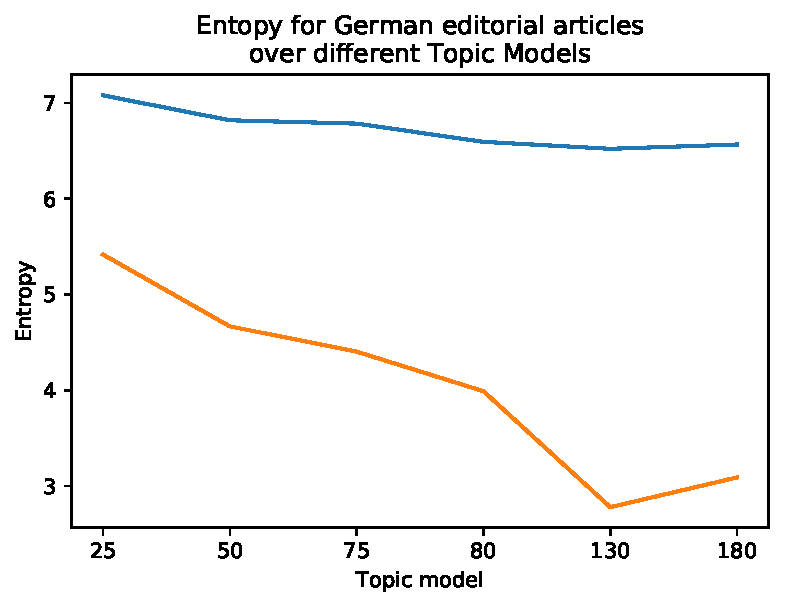
\includegraphics[width=7cm]{gfx/Eval_IC/German_Editorial_Entropy.pdf}
	\end{minipage}
	\caption{Maximal and minimal entropy per topic model for German editorial articles.}
	\label{entr_german}
\end{figure}

\begin{figure}[h]
	\begin{minipage}{0.5\textwidth}
		\centering
		\begin{tabular}[t]{c|cc}
			&max value & min value\\
			\hline
			25 topics&7.029&5.455\\
			50 topics&6.8&4.71\\
			75 topics&6.823&4.636\\
			80 topics&	6.819&4.112\\
			130 topics & 8.741&4.005\\
			180 topics&	8.741&3.249\\
		\end{tabular}
	\end{minipage}%
	\begin{minipage}{0.5\textwidth}
		\centering
		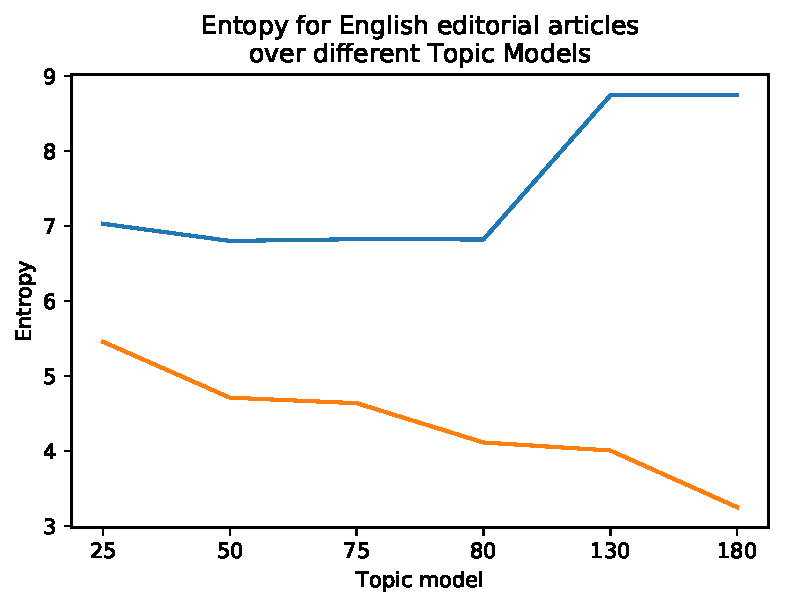
\includegraphics[width=7cm]{gfx/Eval_IC/English_Editorial_Entropy.pdf}
	\end{minipage}
	\caption{Maximal and minimal entropy values per topic model for English editorial articles.}
	\label{entr_english}
\end{figure}

\subsubsection{Alpha}

In Figure \ref{alpha_ger} the alpha values for \textit{German editorial articles} are shown. The maximal alpha values as well the minimal alpha values are decreasing. This indicates, that the documents are described by fewer topics with a higher probability. But alpha does not say anything about the topic quality, so the few topics, which are assigned to the document can be rather general or specific. Therefore, we calculated the entropy for the topic with the maximal alpha value 0.186 from the topic model with 25 topics and the minimal alpha value 0.002 from the topic model with 240 topics. We got the entropy value of 7.08 for the topic model with 25 topics and the entropy value of 6.28 for the topic model with 240 topics. So the document with the highest alpha value consists out of either general topics and the document with the lowest alpha value out of specific ones. 

The minimal alpha values for \textit{English editorial articles} (Figure \ref{alpha_eng}) are continuously declining up to the topic model with 130 topics. Then the alpha value is staying the same. The maximal alpha values are volatile, so there is no prediction possible, if the values will raise or fall again.
\begin{figure}[h]
	\begin{minipage}{0.5\textwidth}
		\centering
		\begin{tabular}[t]{c|cc}
			&max value & min value\\
			\hline
			25 topics&0.186&0.027\\
			50 topics&0.104&0.015\\
			75 topics&0.065&0.011\\
			140 topics&	0.061&0.004\\
			190 topics &0.050&0.003\\
			240 topics&	0.046&0.002\\
		\end{tabular}
	\end{minipage}%
	\begin{minipage}{0.5\textwidth}
		\centering
		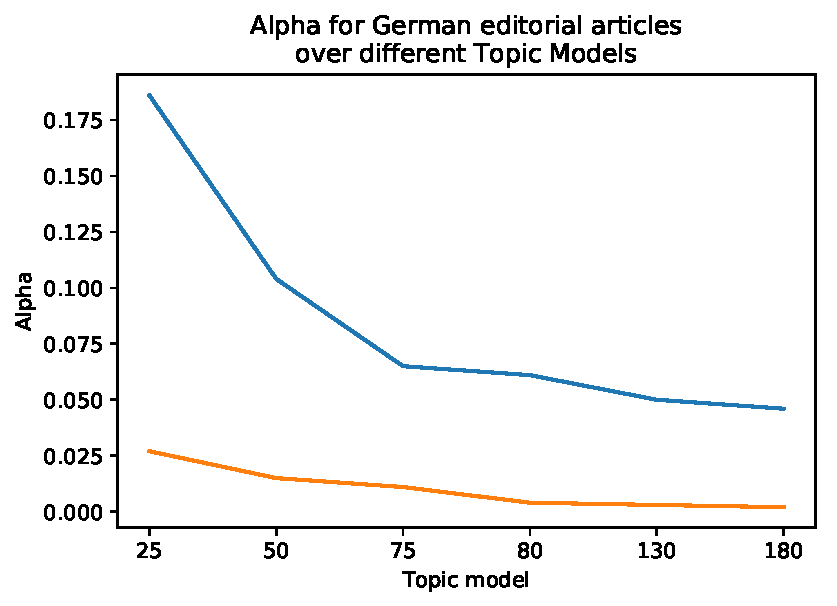
\includegraphics[width=7cm]{gfx/Eval_IC/German_Editorial_Alpha.pdf}
	\end{minipage}
	\caption{Maximal and minimal alpha values per topic model for German editorial articles.}
	\label{alpha_ger}
\end{figure}
\begin{figure}[h]
	\begin{minipage}{0.5\textwidth}
		\centering
		\begin{tabular}[t]{c|cc}
			&max value & min value\\
			\hline
			25 topics&0.159&0.032\\
			50 topics&0.229&0.013\\
			75 topics&0.159&0.010\\
			80 topics&	0.180&0.004\\
			130 topics &0.144&0.002\\
			180 topics&	0.118&0.002\\
		\end{tabular}
	\end{minipage}%
	\begin{minipage}{0.5\textwidth}
		\centering
		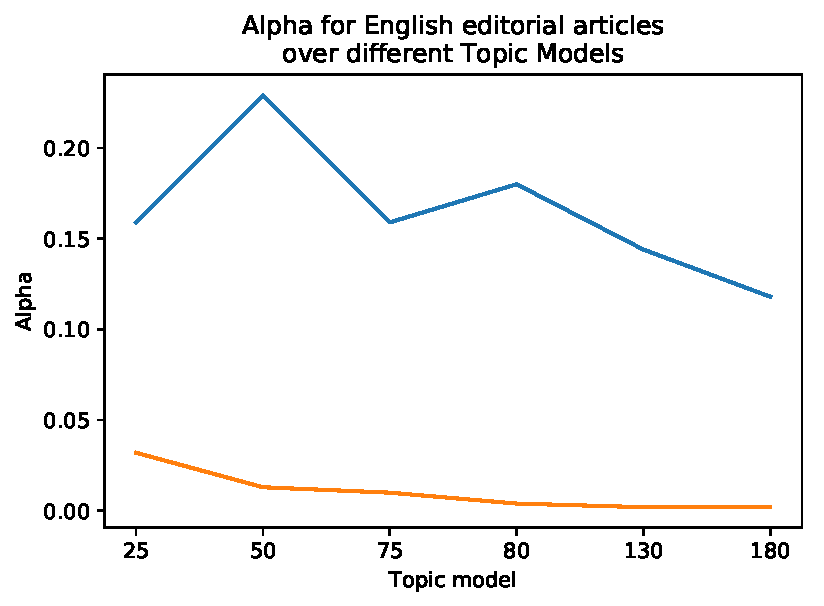
\includegraphics[width=7cm]{gfx/Eval_IC/English_Editorial_Alpha.pdf}
	\end{minipage}
	\caption{Maximal and minimal alpha values per topic model for English editorial articles.}
	\label{alpha_eng}
\end{figure}

\subsubsection{Coherence}

The maximal coherence score is for \textit{German editorial articles} (Figure \ref{eval:coherence_ger}) in the range of the maximal values -0.91 and -1.1 and for \textit{English editorial articles} (Figure \ref{eval:coherence_en}) in the range of -0.49 and -0.56. The maximal values do not change a lot for both datasets, but no pattern how the values are changing can be seen. The same can be said for the minimal coherence values, the only difference is, that the range in which the coherence is moving is much bigger than the range from the maximal values. For \textit{German editorials} it is between -3.96 and -9.2 and for \textit{English editorials} between -2.2 and -16.4.
\begin{figure}[h]
	\begin{minipage}{0.5\textwidth}
		\centering
		\begin{tabular}[t]{c|cc}
			&max value & min value\\
			\hline
			25 topics&-0.994&-3.957\\
			50 topics&-0.999&-5.605\\
			75 topics&-1.102&-6.792\\
			140 topics&	-0.956&-6.661\\
			190 topics &-0.912&-9.19\\
			240 topics&	-0.948&-7.25\\
		\end{tabular}
	\end{minipage}%
	\begin{minipage}{0.5\textwidth}
		\centering
		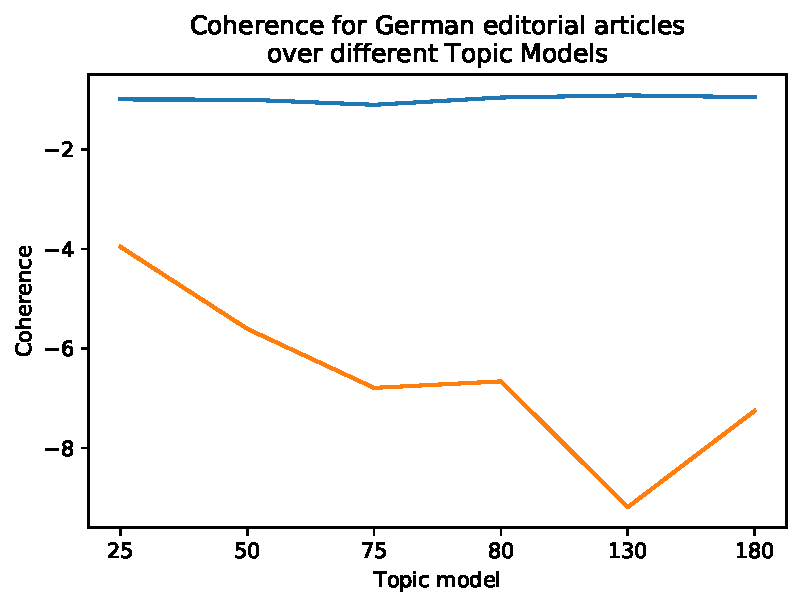
\includegraphics[width=7cm]{gfx/Eval_IC/German_Editorial_Coherence.pdf}
	\end{minipage}
	\caption[]{Maximal and minimal coherence values per topic model for German editorial articles.}
	\label{eval:coherence_ger}
\end{figure}

\begin{figure}[h]
	\begin{minipage}[t]{0.5\textwidth}
		\centering
		\begin{tabular}{c|cc}
			&max value & min value\\
			\hline
			25 topics&-0.557&-2.242\\
			50 topics&-0.568&-9.570\\
			75 topics&-0.505&-5.913\\
			80 topics&	-0.493&-3.666\\
			130 topics &-0.525&-16.257\\
			180 topics&	-0.549&-16.374\\
		\end{tabular}
	\end{minipage}%
	\begin{minipage}{0.5\textwidth}
		\centering
		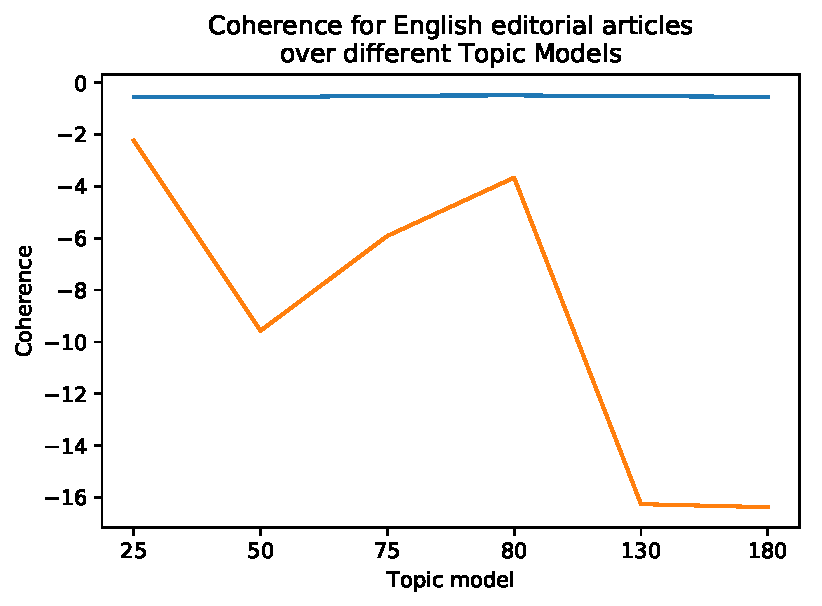
\includegraphics[width=7cm]{gfx/Eval_IC/English_Editorial_Coherence.pdf}
	\end{minipage}
	\caption[]{Maximal and minimal coherence values per topic model for English editorial articles.}
	\label{eval:coherence_en}
\end{figure}

\subsubsection{Theta}

In the following we used the document topic matrix to calculate, in how many documents a certain topic covers more then 10\% of the document and how many topics occur over 10\% in a document. 

First, we start with the number of documents a certain topic covers over 10\%.
In Figure \ref{eval:amount doc_per_topic_ger} one can see, that the maximal and minimal number of documents is decreasing when increasing the topic number for \textit{German editorial articles}. This indicated, that the topics are so specific, that they do not appear in any document with a probability higher then the threshold.

For \textit{English editorial articles} (Figure \ref{eval:amount doc_per_topic_eng}) the maximal number of documents is volatile, whereas the minimal numbers of documents are decreasing and there even seem to be topics, that are not assigned to any document, because they do not cover the meaning of the document over the threshold. 

\begin{figure}[h]
	\begin{minipage}[t]{0.5\textwidth}
		\centering
		\begin{tabular}{c|cc}
			&max value & min value\\
			\hline
			25 topics&1878&154\\
			50 topics&1026&46\\
			75 topics&693&32\\
			140 topics&655&11\\
			190 topics &423&5\\
			240 topics&	352&5\\
		\end{tabular}
	\end{minipage}
	\begin{minipage}{0.5\textwidth}
		\centering
		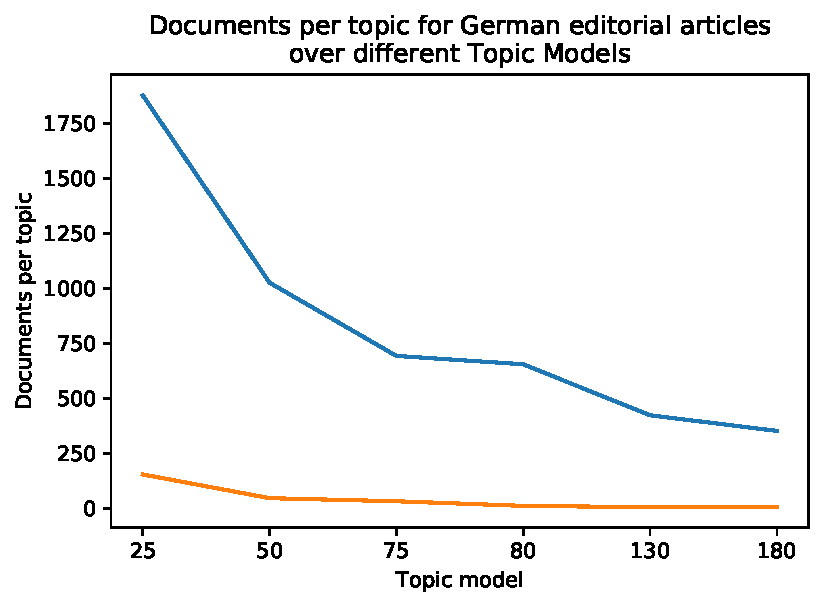
\includegraphics[width=7cm]{gfx/Eval_IC/German_Editorial_Doc_per_topic.pdf}
	\end{minipage}
	\caption[]{Maximal and minimal number of documents containing the same topic for German editorial articles.}
	\label{eval:amount doc_per_topic_ger}
\end{figure}

\begin{figure}[h]
	\begin{minipage}{0.5\textwidth}
		\centering
		\begin{tabular}[t]{c|cc}
			&max value & min value\\
			\hline
			25 topics&788&58\\
			50 topics&589&13\\
			75 topics&435&7\\
			80 topics&636&7\\
			130 topics &292&0\\
			180 topics&	443&0\\
		\end{tabular}
	\end{minipage}
	\begin{minipage}{0.5\textwidth}
		\centering
		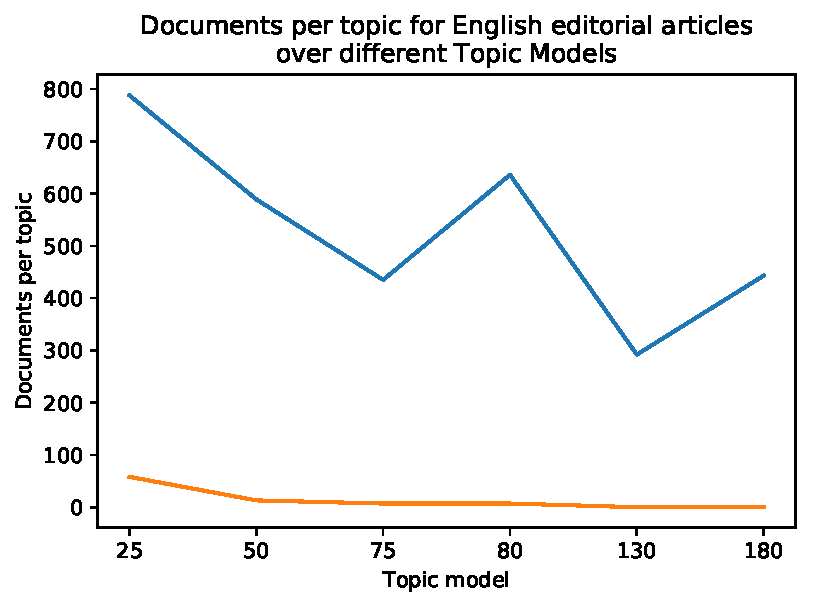
\includegraphics[width=7cm]{gfx/Eval_IC/English_Editorial_Doc_per_topic.pdf}
	\end{minipage}
	\caption[]{Maximal and minimal number of documents containing the same topic for English editorial articles.}
	\label{eval:amount doc_per_topic_eng}
\end{figure}

\begin{figure}
	
	\begin{minipage}[t]{0.5\textwidth}
		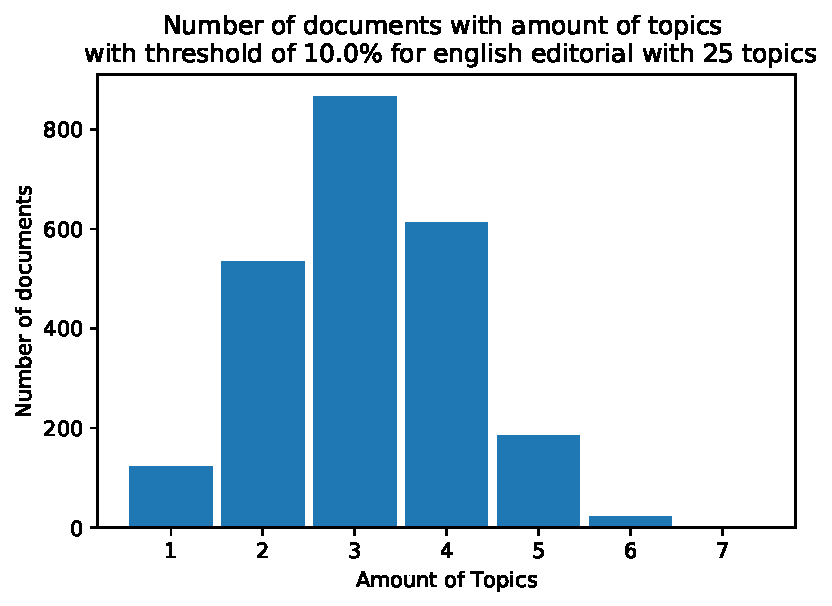
\includegraphics[width=7cm]{gfx/GrafikenFinal/englisheditoriallda_topPerdoc25.pdf}
	\end{minipage}
	\begin{minipage}[t]{0.5\textwidth}
		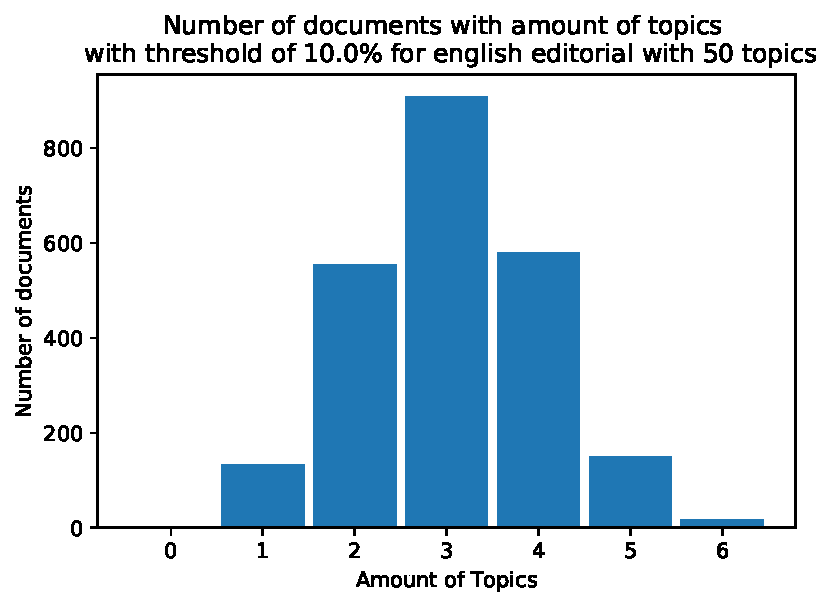
\includegraphics[width=7cm]{gfx/GrafikenFinal/englisheditoriallda_topPerdoc50.pdf}
	\end{minipage}
	\begin{minipage}[t]{0.5\textwidth}
		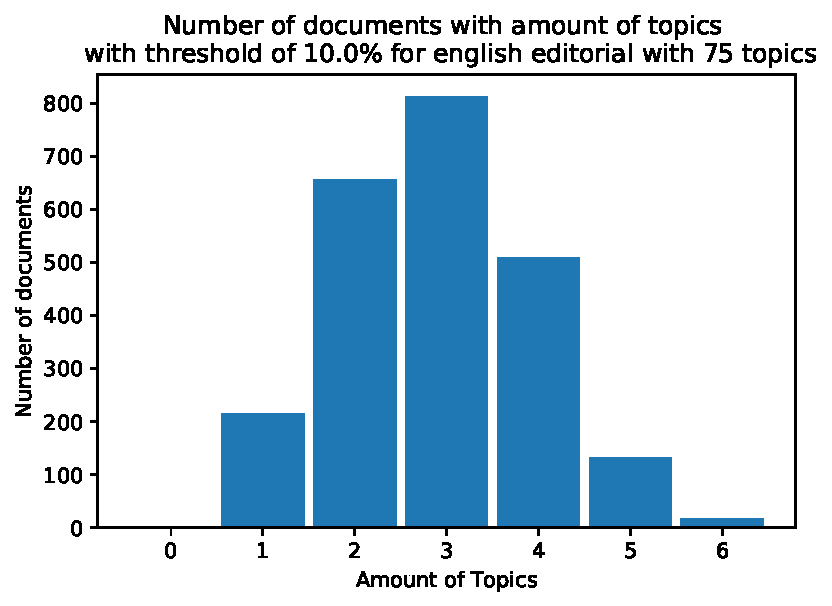
\includegraphics[width=7cm]{gfx/GrafikenFinal/englisheditoriallda_topPerdoc75.pdf}
	\end{minipage}
	\begin{minipage}[t]{0.5\textwidth}
		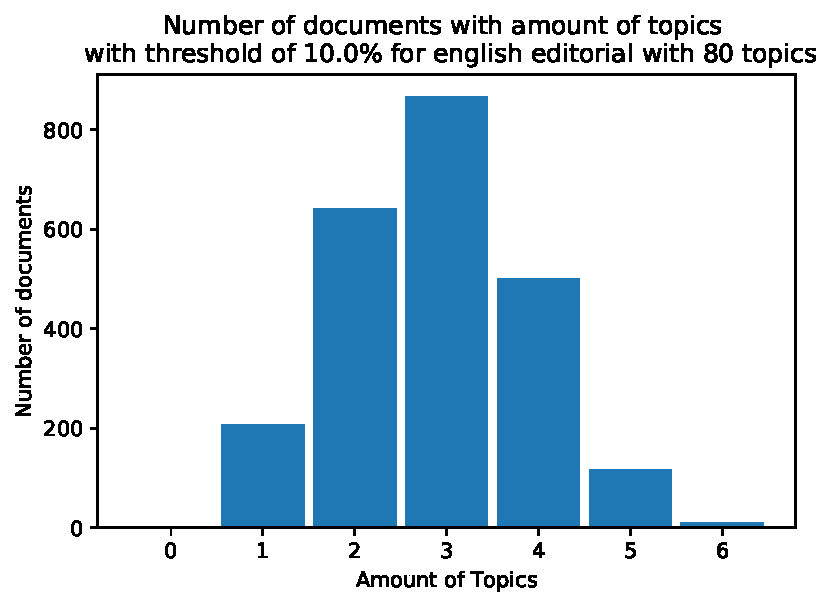
\includegraphics[width=7cm]{gfx/GrafikenFinal/englisheditoriallda_topPerdoc80.pdf}
	\end{minipage}
	\begin{minipage}[t]{0.5\textwidth}
		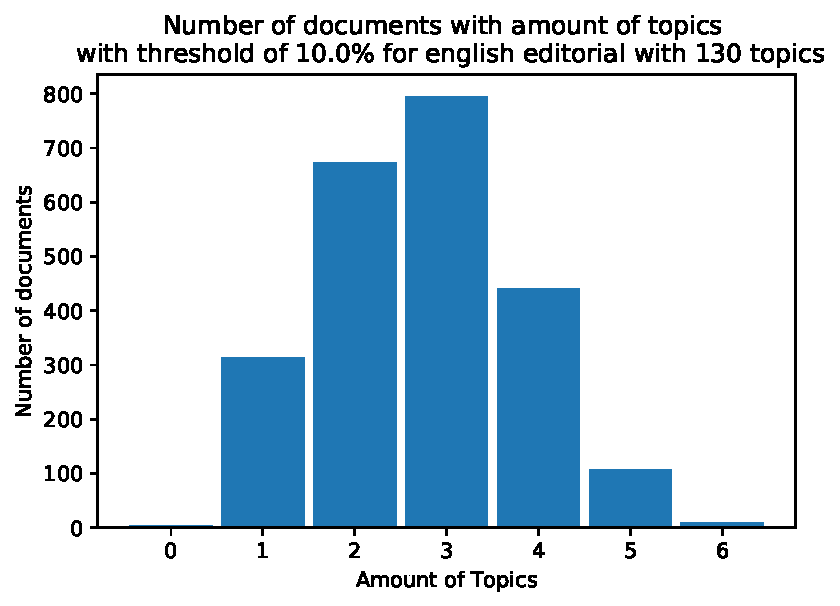
\includegraphics[width=7cm]{gfx/GrafikenFinal/englisheditoriallda_topPerdoc130.pdf}
	\end{minipage}
	\begin{minipage}[t]{0.5\textwidth}
		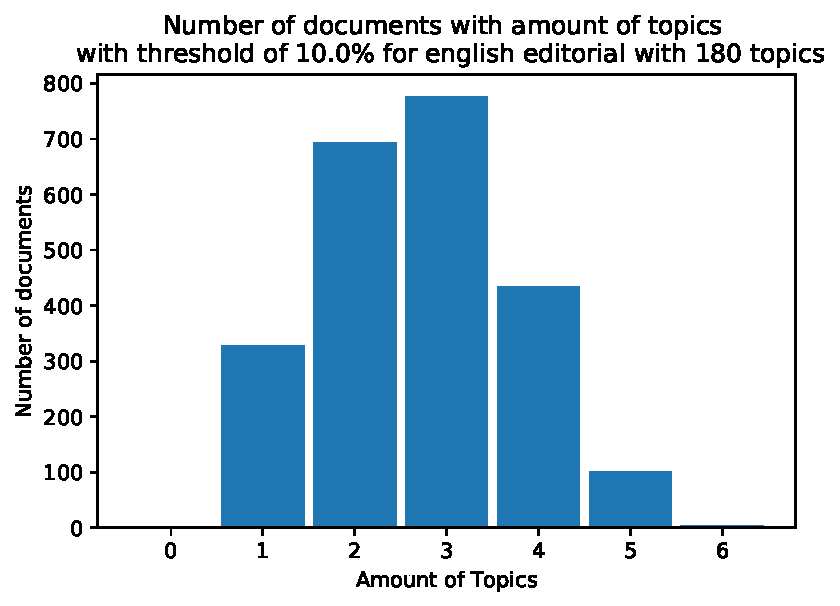
\includegraphics[width=7cm]{gfx/GrafikenFinal/englisheditoriallda_topPerdoc180.pdf}
	\end{minipage}
	\caption{Amount of topics in documents over a threshold of 10\% for English editorial articles}
	\label{top_per_doc_eng}
\end{figure}

\begin{figure}
	\begin{minipage}[t]{0.5\textwidth}
		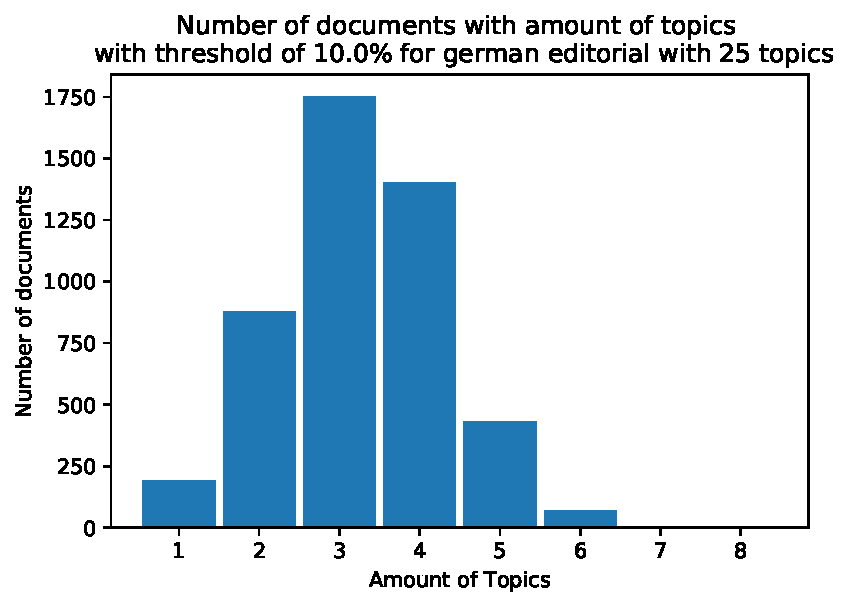
\includegraphics[width=7cm]{gfx/GrafikenFinal/germaneditoriallda_topPerdoc25.pdf}
	\end{minipage}
	\begin{minipage}[t]{0.5\textwidth}
		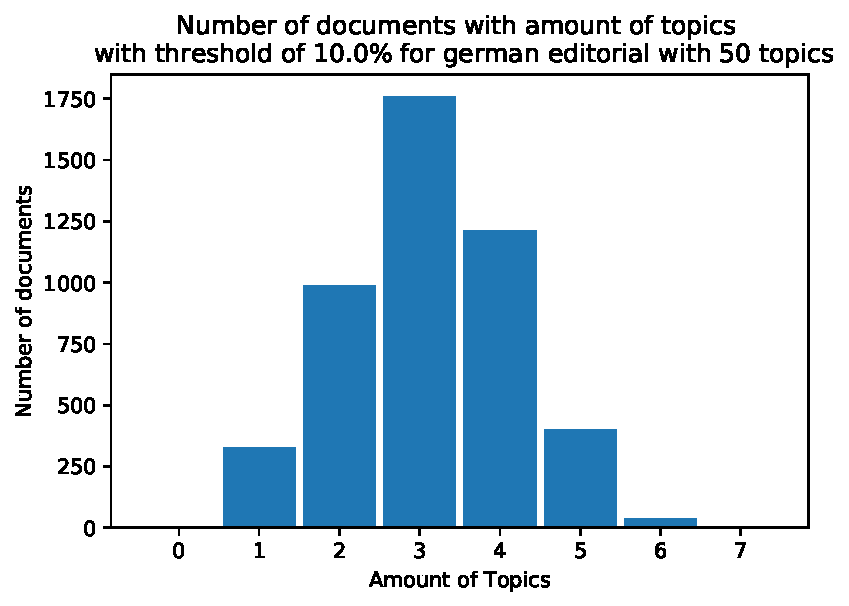
\includegraphics[width=7cm]{gfx/GrafikenFinal/germaneditoriallda_topPerdoc50.pdf}
	\end{minipage}
	\begin{minipage}[t]{0.5\textwidth}
		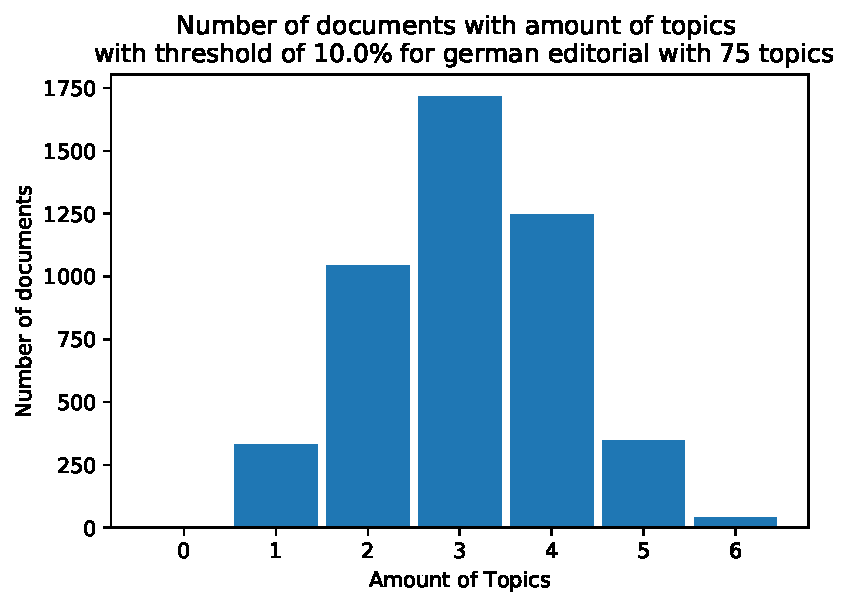
\includegraphics[width=7cm]{gfx/GrafikenFinal/germaneditoriallda_topPerdoc75.pdf}
	\end{minipage}
	\begin{minipage}[t]{0.5\textwidth}
		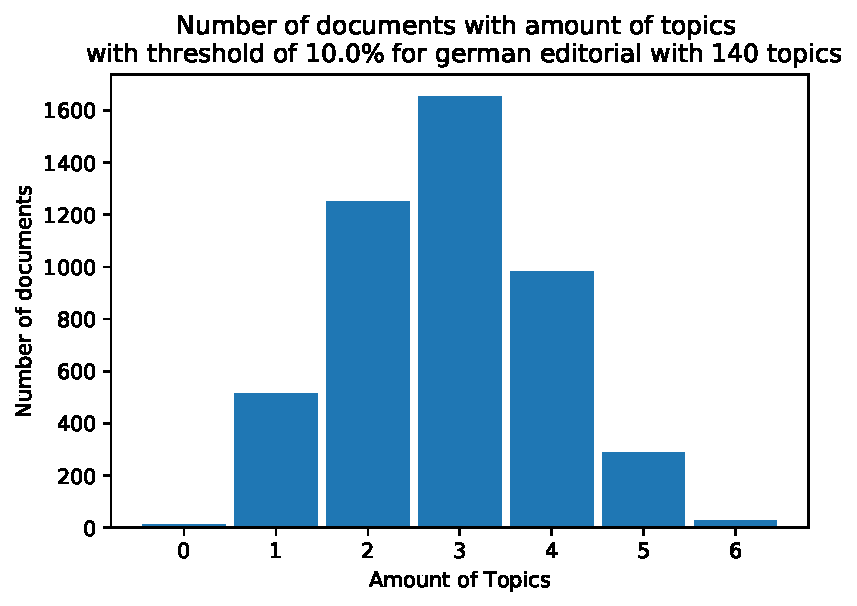
\includegraphics[width=7cm]{gfx/GrafikenFinal/germaneditoriallda_topPerdoc140.pdf}
	\end{minipage}
	\begin{minipage}[t]{0.5\textwidth}
		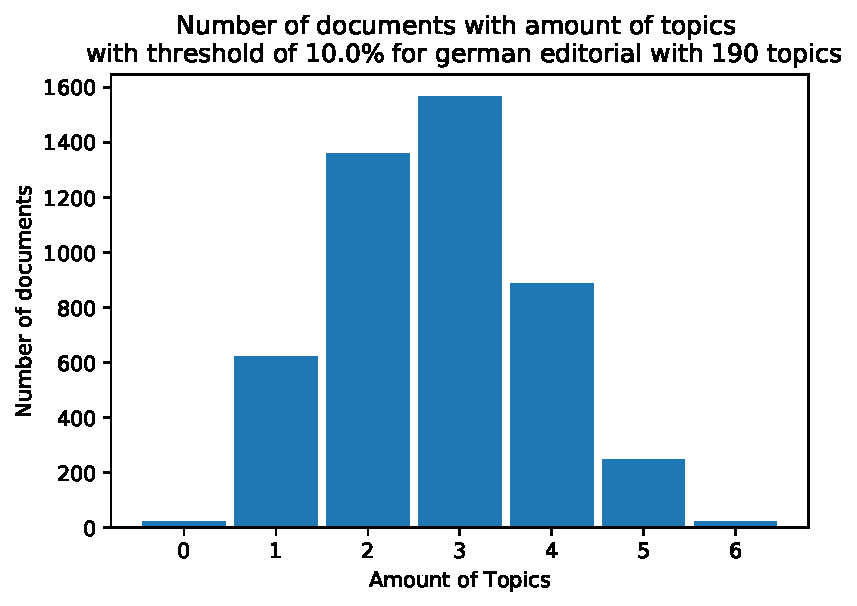
\includegraphics[width=7cm]{gfx/GrafikenFinal/germaneditoriallda_topPerdoc190.pdf}
	\end{minipage}
	\begin{minipage}[t]{0.5\textwidth}
		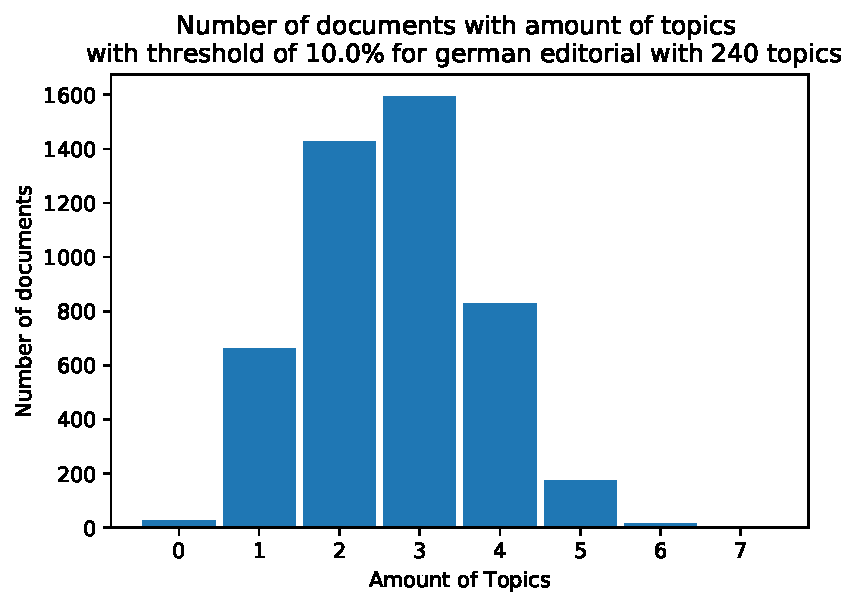
\includegraphics[width=7cm]{gfx/GrafikenFinal/germaneditoriallda_topPerdoc240.pdf}
	\end{minipage}
	\caption[]{Amount of topics in documents over a threshold of 10\% for German editorial articles}
	\label{top_per_doc_ger}
\end{figure}

Second, we analyzed how many topics occur in a document over 10\%. 
The plots in Figure \ref{top_per_doc_ger} and \ref{top_per_doc_eng} represent the number of documents with the number of topics over the threshold. On the x-axis the amount of topics, which are occurring over 10\%in a document, while the y-axis represents the number of documents, which include a certain amount of topics. 

In Figure \ref{top_per_doc_eng} is shown how the number of topics for \textit{English editorial articles} change. When increasing the number from 25 to 50 topics, all documents are modeled by a most 6 topics. This means, that with a higher topic number the topics are more tailored to documents and thus the documents can be represented with less topics. This is also supported by the observation, that the number of documents, that contain only one or two topics over the threshold are slightly increasing with the number of topics. At the same time there are some documents, that do not express any topic over the threshold, which could indicate, that these documents are rather general and cover many topics with a low probability, instead of covering a few specific topics.
 %Across all plots the maximal number of topics, occurring in a document is 3 and does not change. Only the number of documents decreases from above 850 documents to about 780 documents. From the plots with 130 to 180 topics no significant changes can be seen. One can deduce from the plots, that the topics are getting more specific. 
For the \textit{German editorial articles} in Figure \ref{top_per_doc_ger} it can be seen, that the maximal number of topics, covering a document is also at 3. From the topic model with 25 topics to 50 topics, there are no documents, which include 8 topics, but there are documents, that do not contain any topic. When increasing the number of topics to the next level, there are no documents, which contain 7 topics. In the next plots, the number of documents containing 2, only 1 or no topic is raising, but the maximal topic number remains 3. The last plot is looking nearly the same apart from adding a few documents with 7 topics. For this dataset it could be said, that the topics are getting up to 190 topics more specific. With more topics the number of generic topics increases. So the topic model with 190 seems the best for obtaining good topics.


\subsubsection{Jensen Shannon divergence}

The \ac{JS} divergence was used to calculate the similarity of topics based on the topic term matrix in a topic model and across topic models. The similarities were then visualized as heat maps. The dark red colored boxes express high similarity, while the brighter boxes express a smaller similarity.  
The topic models form \textit{German editorial articles} with 25, 50 and 70 topics were evaluated manually. The highest similarities (dark red) with the values of 0.63, 0.65, and 0.65 for the topics intra a topic model were taken, and the topics were compared with each other in Table \ref{intra_topic}. The same words form the top 10 terms of a topic were marked in bold. In Table \ref{inter_topic} the similarities of the topics were calculated across different topic models with 25/50, 50/57 and 50/75 topics. The values for the similarity were 0.9, 0.87 and 0.94. One can see, that the number of common words and the calculated similarity, is much higher in the inter topic model evaluation. This means, that the topics inter a topic model are not as similar to each other as the topics developing across topic models. At least this is not recognizable by the top 10 words of a topic. The heat maps for the inter topic model and intra topic model evaluation can be seen in Figure \ref{heatmap:inter_ger} and \ref{heatmap:intra_ger}.
%TODO heatmaps in anhang

Within the different topic models the topics are hardly similar. This is a good characteristic, because it shows, that the topic number was not over fitted. Across the topic models there are different topics, but also very similar topics, which is shown in Table \ref{min_max_sim_ger} for \textit{German editorial articles} and in Table \ref{min_max_sim_eng} for \textit{English editorial articles}. This means, when increasing the number of topics, some of the new generated topics do not change much and cover the same themes such as the previous topic model, but new topics are added, too, which cover new themes. By adding new topics the development of the topics can be tracked. 


\begin{table}
	\centering
	\begin{tabular}{c|c|c}
		topics& \multicolumn{2}{c}{compared topics with the highest similarity:}\\
		\hline
		25 & T1:\thead{all, jed, sehen,\\ stehen, leben, einfach, welt,\\finden, frage, bio}&T19:\thead{bauer, landwirt, landwirtschaft,\\ milch, preisen, kuh, betrieb,\\ hof, euro, cent}\\
		\hline
		50 &T42:\thead{essen, lebensmittel, \textbf{jed},\\ fleich, all, kaufen, leben,\\ \textbf{stehen}, ernährung, einfach}&T40:\thead{hof, betreiben, landwirtschaft,\\ \textbf{stehen}, landwirt, bauer, familie,\\ verkaufen, \textbf{jed}, alt}\\
		\hline
		75&T63:\thead{bauer, landwirt, euro,\\ \textbf{preisen}, konventionell, biobauer, geld, \\bekommen, umstellen, ernten}&T67:\thead{product, verbraucher, kunde,\\ deutschland, \textbf{preisen}, deutsch, prozent,\\ handeln,supermarkt, deutsche}
	\end{tabular}
	\caption[]{Compared topics intra a topic model with the highest similarity. Common topic words are \textbf{bold}}
	\label{intra_topic}
\end{table}

\begin{table}
	\centering
	\begin{tabular}{c|c|c}
		topics& \multicolumn{2}{c}{compared topics with the highest similarity:}\\
		\hline
		25/50 & T21:\thead{\textbf{prozent}, \textbf{euro}, \textbf{ökologisch}, \textbf{betrieb},\\ \textbf{hektar}, million, steigen,\\ \textbf{fläche}, deutschland, \textbf{zahlen}}&
			T2:\thead{\textbf{prozent}, \textbf{ökologisch}, \textbf{betrieb}, \textbf{hektar},\\ \textbf{fläche}, landwirtschaft, \textbf{zahlen},\\ anteil, bewirtschaften, \textbf{euro}}\\
			\hline
			50/75 &T4:\thead{\textbf{pestizid}, \textbf{finden}, \textbf{probe}, \textbf{rückstand},\\ \textbf{greenpeace}, konventionell, \textbf{untersuchen}, \\\textbf{belasten}, prozent,einsatz}&T54:\thead{\textbf{pestizid}, \textbf{rückstand}, \textbf{probe}, grenzwert,\\ \textbf{finden}, \textbf{greenpace}, stoff,\\ \textbf{belasten}, \textbf{untersuchen}, einsetzen}\\ 
			\hline
			50/75&T9:\thead{\textbf{eiern}, \textbf{fipronil}, \textbf{belasten}, \textbf{niederlande},\\ \textbf{deutschland}, \textbf{nehmen}, \textbf{verkaufen},\\\textbf{betreffen}, betrieb, angeben}&T57:\thead{\textbf{eiern}, \textbf{fipronil}, \textbf{belasten}, \textbf{niederlande},\\ \textbf{nehmen}, \textbf{deutschland}, \textbf{verkaufen}, \\betroffen, \textbf{betreffen}, behörde}\\
		\end{tabular}
		\caption[]{Compared topics inter topic models with the highest similarity. Common topic words are \textbf{bold}}
		\label{inter_topic}
\end{table}

\begin{figure}
	\begin{minipage}[t]{0.5\textwidth}
		\subfloat[Minimal and maximal similarities for German editorial articles inter different topic models]{
		\begin{tabular}{c|c|c}
			topics & min value &max value\\
			\hline
			25&0.38&0.63\\
			50& 0.35 & 0.65\\
			75&0.33&0.65\\
			140&0.34&0.62\\
			190&0.33&0.61\\
			240&0.33&0.60\\
		\end{tabular}}
	\end{minipage}
	\begin{minipage}[t]{0.5\textwidth}
		\subfloat[Minimal and maximal similarities for German editorial articles intra different topic models]{
		\begin{tabular}{c|c|c}
			topics & min value &max value\\
			\hline
			25/50&0.35&0.91\\
			25/75& 0.35 & 0.88\\
			50/75&0.35&0.94\\
			140/190&0.33&0.88\\
			140/240&0.32&0.92\\
			190/240&0.33&0.91\\
		\end{tabular}}
	\end{minipage}
\caption[]{Minimal and maximal similarities inter and intra topic models for German editorial articles}
\label{min_max_sim_ger}
\end{figure}


\begin{figure}
	\begin{minipage}[t]{0.5\textwidth}
		\subfloat[Minimal and maximal similarities for English editorial articles inter different topic models]{
			\begin{tabular}{c|c|c}
				topics & min value &max value\\
				\hline
				25&0.42&0.66\\
				50& 0.36 & 0.68\\
				75&0.35&0.69\\
				80&0.35&0.67\\
				130&0.34&0.65\\
				180&0.36&0.67\\
			\end{tabular}
			}
	\end{minipage}
	\begin{minipage}[t]{0.5\textwidth}
		\subfloat[Minimal and maximal similarities for English editorial articles intra different topic models]{
		\begin{tabular}{c|c|c}
			topics & min value &max value\\
			\hline
			25/50&0.39&0.90\\
			25/75& 0.37 & 0.91\\
			50/75&0.35&0.91\\
			80/130&0.34&0.95\\
			80/180&0.33&0.97\\
			130/180&0.33&1.0\\
		\end{tabular}}
	\end{minipage}
	\caption{Minimal and maximal similarities inter and intra topic models for English Editorial articles}
	\label{min_max_sim_eng}
\end{figure}



\subsubsection{Correlation}
Calculating the correlation between every key figure, the relationship over the different topic models is analyzed by using the Pearson correlation. It is a measure of the linear correlation between two variables $X$ and $Y$ and can assume values between 1 an -1, where 1 represents a total positive linear correlation, 0 no linear correlation and -1 represents a total negative linear correlation. 

In Figure \ref{Corr} the correlation for the key figures alpha, entropy, coherence and documents per topic is calculated. 
On the x-axis the topic models with different topics is shown, while the y-axis shows the calculated correlation.

One can see, that the alpha and documents per topic values are correlating. This is, because both 
measure the sparsity of a topic over documents in a corpus. The alpha values, coherence values and documents
per topic values hardly correlate. From this one can deduce, that the topics, which are most present 
in a document are not so easily interpretable for humans. Furthermore, all correlations including 
entropy are at the beginning highly correlating, but the correlation coefficient is continuously decreasing. 
So entropy in general seem to be a metric, which is developing independently form the other key
figures, so from the characteristic, if a topic is rather general or specific, can not be deduced, 
if the topic is strongly represented in a document or if it is easily interpretable.

\begin{figure}
	\begin{minipage}[t]{0.5\textwidth}
	\subfloat[Correlation for German editorial articles]{
	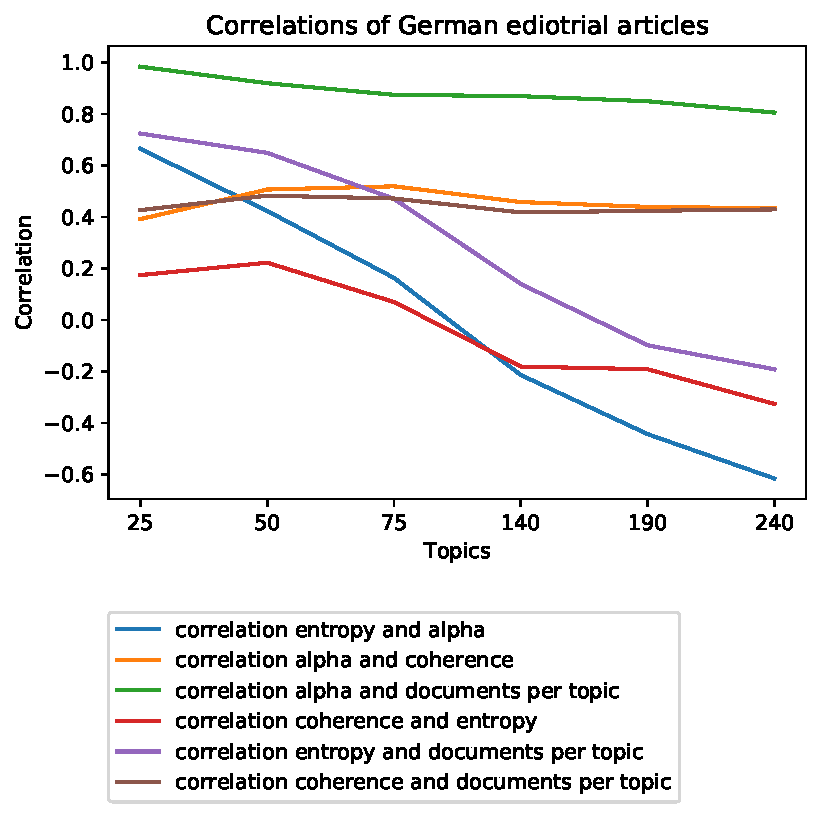
\includegraphics[width=7cm]{gfx/Correlation/6Cor_germ.pdf}}
	\end{minipage}
	\begin{minipage}[t]{0.5\textwidth}
		\subfloat[Correlation for English editorial articles]{
	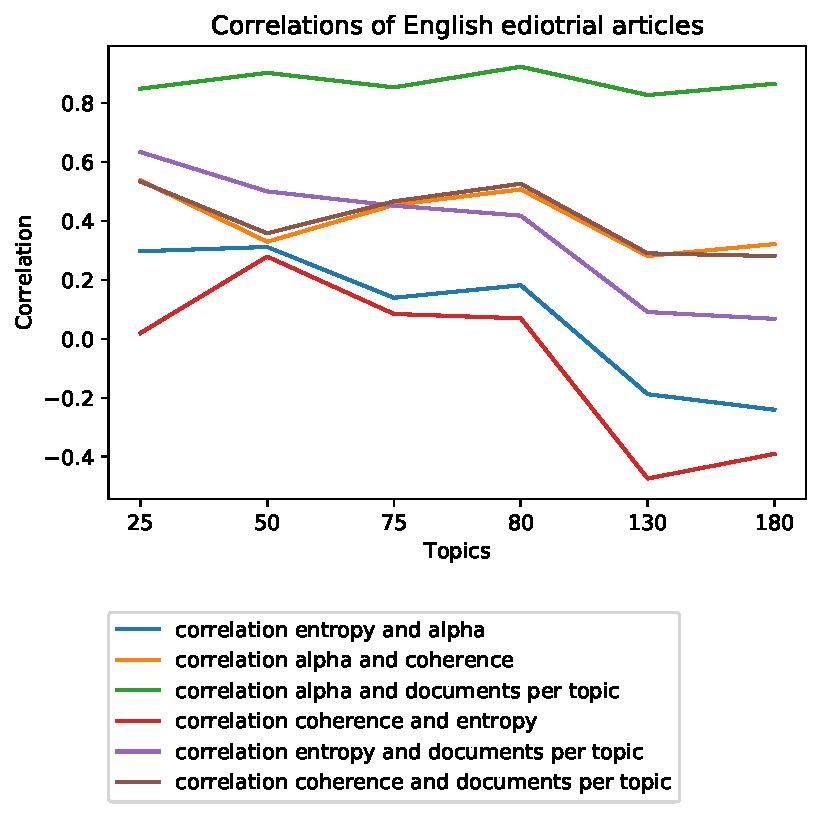
\includegraphics[width=7cm]{gfx/Correlation/6Cor_eng.pdf}}
	\end{minipage}
\caption[]{Correlations of key figures for German and English editorial articles}
\label{Corr}
\end{figure}

The analysis of the different key figures on the two datasets has shown that no key figure on its own is enough to determine the quality or the optimal topic number. When considering multiple key figures, it is possible to compare different topic models based on how generic or specific the topics are (entropy) or how the topics are distributed across the corpus (alpha). It is not possible, however, to compare topic models of different datasets. Each dataset has its own characteristics such as the number of documents, the average length of the documents or how specific the topics are covered. These differences make it impossible to compare topic models trained on different datasets. 

%resume: besten kriterien lassen sich nicht so leich bestimmen. da es vom datensatz abhägen kann, aus wie vielen dokumenten besteht der corpus, wie lang sind diese documente. und wie spezifisch sind die themen, die in einem document behandelt werden.



\newpage
\chapter{Future Work and Conclusion}
\label{future_work}

\section{Future work}
As this thesis covered multiple areas in the field of topic modeling, the recommendations for possible future improvements are also divided into two sections. We have applied the intrinsic automatic topic labeling technique of \cite{Mei2007}. The authors propose several possible improvements that would also improve the labeling on our data. Foremost, a different method for generating canidate labels and matching these to topics is necessary. The extrinsic labeling approach relied on WordNet and could thus only be applied on the English data. The methods could be extended to support German data, for example by incorporating GermaNet or other lexical sources. Lastly, it would be interesting to generate labels for hierarchical topic models.

In this thesis the internal consistency of topic models was studied to analyze the quality of the topics and what effect the chosen number of topics has. In future revisions also the effect of changing other parameters such as the priors $\alpha$ and $\beta$ for LDA on the quality of the modeling should be considered.

\section{Conclusion}
In this thesis two main topics were covered: How can we label topics automatically and how can we measure the internal consistency of topic modeling. 

To answer the fist question the intrinsic and extrinsic automatic topic labeling was introduced an evaluated on English and German editorial articles. The evaluation showed, that the intrinsic approach produced meaningful labels on their own, but theses did not fit to the topics. The extrinsic approach was more successful.
On average with this method labels were generated, which were fitting more to the topics and some of the automatic labels even matched with the labels, that were submitted by the domain experts. 

To answer the second question, several key figures were introduced to measure the internal consistency of topic models with a different number of topic numbers. All key figures were applied on our datasets. It was determined that a single key figure is not enough to specify the number of topics or the quality of the topics. When comparing topic models that were trained on the same dataset, however, the key figures can be used to evaluate which model has more generic or specific topics and how the topics change when varying the number of topics.

 % Weitere Kapitel hier einfügen 

% --------------------------
% Back matter
% --------------------------
\appendix\cleardoublepage
% !TEX root = ../my-thesis.tex
%
\chapter{Descriptive Statistics of the Dataset}
\label{app:descriptiv_stats}
\begin{figure}[h]
	\begin{center}
		%
		\subfloat[Number of Articles per Type]{%
			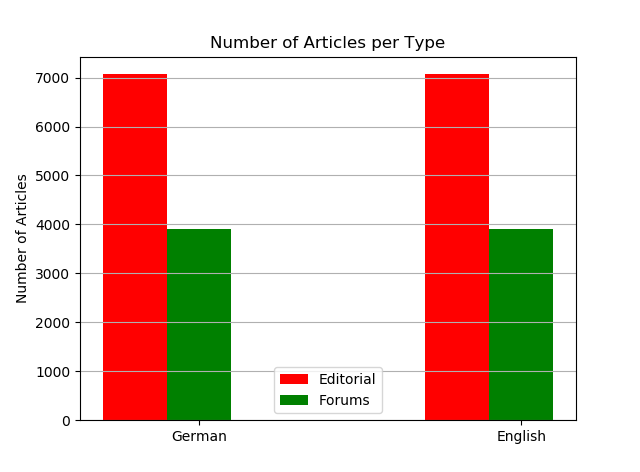
\includegraphics[width=0.5\textwidth]{gfx/descriptive_statistics/Number_of_articles_per_type.png}
		}%
		\subfloat[Number of Comments per Type]{%
			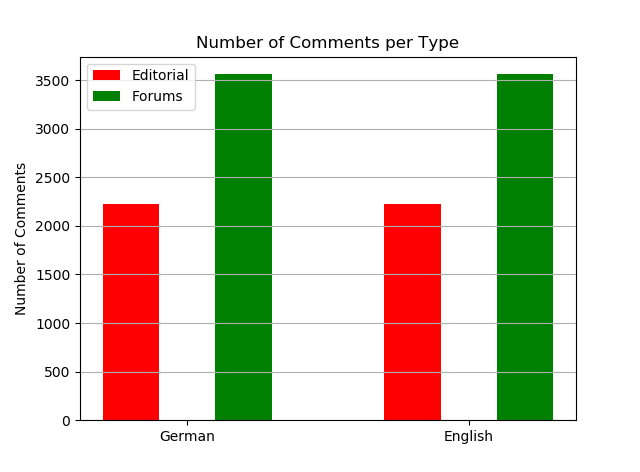
\includegraphics[width=0.5\textwidth]{gfx/descriptive_statistics/Number_of_comments_per_type.png}
		}\\ %  ------- End of the first row ----------------------%
		\subfloat[Distribution of English articles per year]{%
			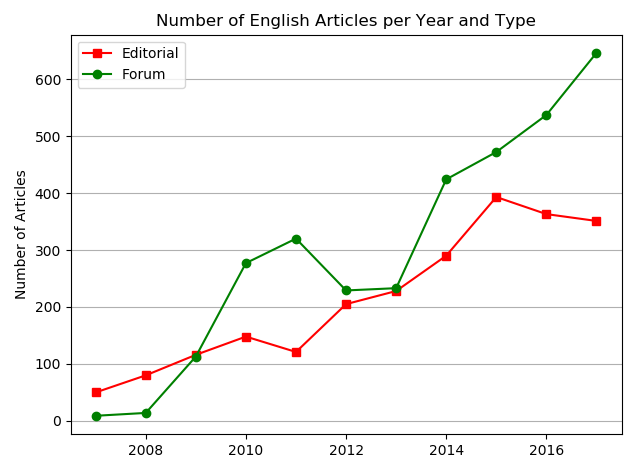
\includegraphics[width=0.5\textwidth]{gfx/descriptive_statistics/Number_of_english_articles_per_year_and_type.png}
		}%
		\subfloat[Distribution of German articles per year]{%
			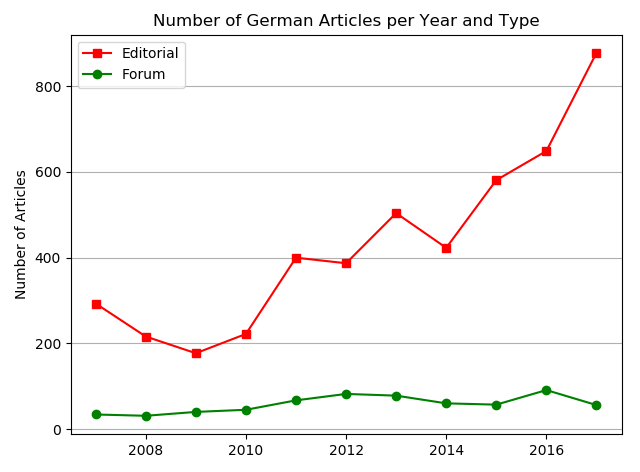
\includegraphics[width=0.5\textwidth]{gfx/descriptive_statistics/Number_of_Germna_articles_per_year_and_type.png}
		}%
		%
	\end{center}
	\caption{Descriptive Statistics for all datasets}
	\label{fig:descriptive_stats}
\end{figure}

\section{Detailed Statistics of all Sources}
% English Editorial
\begin{sidewaystable}
	\begin{tabular}{lrrrrrr}
		\toprule
		Source           & Total articles & Relevant articles & \% rel. articles & Avg. article length\footnotemark[1] & Rel. art. w/ cmnt. & \% rel. art. w/ cmnt. \\ \midrule
		usatoday         &             95 &                61 &            64.21 &                 303 &                 15 &                 24.59 \\
		nytimes          &            438 &               327 &            74.66 &                 528 &                 99 &                 30.28 \\
		nypost           &            106 &                33 &            31.13 &                 377 &                  0 &                  0.00 \\
		washingtonpost   &           1563 &               489 &            31.29 &                 480 &                285 &                 58.28 \\
		latimes          &           1522 &               270 &            17.74 &                 419 &                  8 &                  2.96 \\
		chicagotribune   &           2283 &               572 &            25.05 &                 420 &                 39 &                  6.82 \\
		huffingtonpost   &            880 &               668 &            75.91 &                 479 &                  0 &                  0.00 \\
		organicauthority &             66 &                43 &            65.15 &                 626 &                  0 &                  0.00 \\ \bottomrule
	\end{tabular}
	\caption{Article statistics for English editorial data} 
	\begin{tabular}{lrrrrrrr}
		\toprule
		Source           & Total comments & Relevant comments & \% rel. cmnt. & Root cmnt. & \% root cmnt. & Avg. \# cmnt. & Avg. cmnt. length\footnotemark[1] \\ \midrule
		usatoday         &            259 &               195 &         75.29 &        103 &         52.82 &             3 &                17 \\
		nytimes          &          16128 &             11576 &         71.78 &       7353 &         63.52 &            35 &                40 \\
		nypost           &              0 &                 0 &          0.00 &          0 &          0.00 &             0 &                 0 \\
		washingtonpost   &          84669 &             14875 &         17.57 &       6667 &         44.82 &            30 &                24 \\
		latimes          &            374 &                14 &          3.74 &         12 &         85.71 &             0 &                34 \\
		chicagotribune   &            281 &               154 &         54.80 &        131 &         85.06 &             0 &                19 \\
		huffingtonpost   &              0 &                 0 &          0.00 &          0 &          0.00 &             0 &                 0 \\
		organicauthority &              0 &                 0 &          0.00 &          0 &          0.00 &             0 &                 0 \\ \bottomrule
	\end{tabular}
	
	\caption{Comment statistics for English editorial data} 
\end{sidewaystable}

% English forums
\begin{sidewaystable}
	\begin{tabular}{lrrrrrr}
		\toprule
		Source         & Total articles & Relevant articles & \% rel. articles & Avg. article length\footnotemark[1] & Rel. art. w/ cmnt. & \% rel. art. w/ cmnt. \\ \midrule
		reddit         &            256 &               225 &            87.89 &                  49 &                190 &                 84.44 \\
		usmessageboard &            382 &                61 &            15.97 &                   0 &                 61 &                100.00 \\
		cafemom        &             88 &                26 &            29.55 &                 251 &                 26 &                100.00 \\
		quora          &           1703 &              1497 &            87.90 &                   5 &               1304 &                 87.11 \\
		fb             &           5035 &              1467 &            29.14 &                  23 &               1355 &                 92.37 \\ \bottomrule
	\end{tabular}
	
	\caption{Article statistics for English forum data} 
	\begin{tabular}{lrrrrrrr}
		\toprule
		Source         & Total comments & Relevant comments & \% rel. cmnt. & Root cmnt. & \% root cmnt. & Avg. \# cmnt. & Avg. cmnt. length\footnotemark[1] \\ \midrule
		reddit         &           9291 &              8392 &         90.32 &       1574 &         18.76 &            37 &                25 \\
		usmessageboard &          78303 &              1982 &          2.53 &       1254 &         63.27 &            32 &                43 \\
		cafemom        &           2206 &               352 &         15.96 &        280 &         79.55 &            13 &                30 \\
		quora          &           9606 &              8699 &         90.56 &       5229 &         60.11 &             5 &                46 \\
		fb             &         299126 &             81660 &         27.30 &      64183 &         78.60 &            55 &                11 \\ \bottomrule
	\end{tabular}
	\caption{Comment statistics for English forum data} 
\end{sidewaystable}

\begin{sidewaystable}
	\begin{tabular}{lrrrrrr}
		\toprule
		Source             & Total articles & Relevant articles & \% rel. articles & Avg. article length\footnotemark[1] & Rel. art. w/ cmnt. & \% rel. art. w/ cmnt. \\ \midrule
		spiegel            &            468 &               152 &            32.48 &                 376 &                 61 &                 40.13 \\
		zeit               &            154 &                62 &            40.26 &                 461 &                 35 &                 56.45 \\
		welt               &            729 &               392 &            53.77 &                 323 &                 35 &                  8.93 \\
		taz                &           2458 &              1406 &            57.20 &                 255 &                249 &                 17.71 \\
		tagesspiegel       &            625 &               278 &            44.48 &                 279 &                 41 &                 14.75 \\
		handelsblatt       &            567 &               286 &            50.44 &                 302 &                 65 &                 22.73 \\
		freitag            &             16 &                 7 &            43.75 &                 678 &                  5 &                 71.43 \\
		tagesschau         &             61 &                17 &            27.87 &                 202 &                 17 &                100.00 \\
		br                 &            191 &                93 &            48.69 &                 297 &                 26 &                 27.96 \\
		wdr                &             68 &                37 &            54.41 &                 241 &                  0 &                  0.00 \\
		swr                &            164 &                82 &            50.00 &                 207 &                  0 &                  0.00 \\
		ndr                &             18 &                 5 &            27.78 &                 209 &                  0 &                  0.00 \\
		derstandard        &           1092 &               646 &            59.16 &                 231 &                529 &                 81.89 \\
		diepresse          &            304 &               152 &            50.00 &                 230 &                100 &                 65.79 \\
		kurier             &            287 &               165 &            57.49 &                 199 &                 88 &                 53.33 \\
		nachrichtenat      &            254 &               134 &            52.76 &                 198 &                 75 &                 55.97 \\
		salzburgcom        &            154 &                93 &            60.39 &                 177 &                  0 &                  0.00 \\
		krone              &             97 &                31 &            31.96 &                 143 &                  0 &                  0.00 \\
		tagesanzeiger      &            187 &                32 &            17.11 &                 171 &                 17 &                 53.12 \\
		nzz                &            316 &               108 &            34.18 &                 338 &                 17 &                 15.74 \\
		aargauer           &            110 &                46 &            41.82 &                 221 &                 17 &                 36.96 \\
		luzernzeitung      &            105 &                55 &            52.38 &                 217 &                  0 &                  0.00 \\
		srf                &            147 &                85 &            57.82 &                 194 &                 56 &                 65.88 \\
		forum\_ernaehrung  &             18 &                 3 &            16.67 &                 339 &                  0 &                  0.00 \\
		heise              &             33 &                17 &            51.52 &                 479 &                 17 &                100.00 \\
		eatsmarter         &            300 &               100 &            33.33 &                 176 &                 35 &                 35.00 \\
		huffingtonpost\_de &            293 &                94 &            32.08 &                 248 &                  0 &                  0.00 \\
		waz                &            744 &               207 &            27.82 &                 193 &                 68 &                 32.85 \\
		merkur             &            393 &               243 &            61.83 &                 209 &                 69 &                 28.40 \\
		rp                 &            604 &               267 &            44.21 &                 204 &                103 &                 38.58 \\
		focus              &            777 &               397 &            51.09 &                 176 &                154 &                 38.79 \\
		campact            &             61 &                23 &            37.70 &                 224 &                 23 &                100.00 \\ \bottomrule
	\end{tabular}
	\caption{Article statistics for German editorial data} 
\end{sidewaystable}

\begin{sidewaystable}	
	\begin{tabular}{lrrrrrrr}
		\toprule
		Source             & Total comments & Relevant comments & \% rel. cmnt. & Root cmnt. & \% root cmnt. & Avg. \# cmnt. & Avg. cmnt. length\footnotemark[1] \\ \midrule
		spiegel            &          62860 &             21551 &         34.28 &       5863 &         27.21 &           141 &                48 \\
		zeit               &           8496 &              2977 &         35.04 &       1279 &         42.96 &            48 &                32 \\
		welt               &           1448 &               528 &         36.46 &        316 &         59.85 &             1 &                21 \\
		taz                &           5537 &              2608 &         47.10 &       1310 &         50.23 &             1 &                28 \\
		tagesspiegel       &           3535 &              1279 &         36.18 &       1279 &        100.00 &             4 &                36 \\
		handelsblatt       &            923 &               295 &         31.96 &        222 &         75.25 &             1 &                28 \\
		freitag            &            129 &                65 &         50.39 &         33 &         50.77 &             9 &                34 \\
		tagesschau         &           4377 &               841 &         19.21 &        841 &        100.00 &            49 &                32 \\
		br                 &            386 &               343 &         88.86 &        220 &         64.14 &             3 &                26 \\
		wdr                &              0 &                 0 &          0.00 &          0 &          0.00 &             0 &                 0 \\
		swr                &              0 &                 0 &          0.00 &          0 &          0.00 &             0 &                 0 \\
		ndr                &              0 &                 0 &          0.00 &          0 &          0.00 &             0 &                 0 \\
		derstandard        &          80715 &             50790 &         62.93 &      12152 &         23.93 &            78 &                15 \\
		diepresse          &           3015 &              1796 &         59.57 &        891 &         49.61 &            11 &                22 \\
		kurier             &            870 &               471 &         54.14 &        308 &         65.39 &             2 &                17 \\
		nachrichtenat      &           1992 &               678 &         34.04 &        310 &         45.72 &             5 &                14 \\
		salzburgcom        &              0 &                 0 &          0.00 &          0 &          0.00 &             0 &                 0 \\
		krone              &              0 &                 0 &          0.00 &          0 &          0.00 &             0 &                 0 \\
		tagesanzeiger      &           4872 &              1139 &         23.38 &        664 &         58.30 &            35 &                18 \\
		nzz                &            622 &               162 &         26.05 &        101 &         62.35 &             1 &                32 \\
		aargauer           &            397 &               262 &         65.99 &        122 &         46.56 &             5 &                18 \\
		luzernzeitung      &              0 &                 0 &          0.00 &          0 &          0.00 &             0 &                 0 \\
		srf                &           1477 &               941 &         63.71 &        652 &         69.29 &            11 &                20 \\
		forum\_ernaehrung  &              0 &                 0 &          0.00 &          0 &          0.00 &             0 &                 0 \\
		heise              &           3636 &              1835 &         50.47 &        335 &         18.26 &           107 &                53 \\
		eatsmarter         &           1179 &               162 &         13.74 &        146 &         90.12 &             1 &                30 \\
		huffingtonpost\_de &              0 &                 0 &          0.00 &          0 &          0.00 &             0 &                 0 \\
		waz                &           1827 &               459 &         25.12 &        327 &         71.24 &             2 &                25 \\
		merkur             &            699 &               347 &         49.64 &        194 &         55.91 &             1 &                15 \\
		rp                 &           1808 &               822 &         45.46 &        822 &        100.00 &             3 &                35 \\
		focus              &           5806 &              2477 &         42.66 &       2123 &         85.71 &             6 &                24 \\
		campact            &           2577 &               687 &         26.66 &        518 &         75.40 &            29 &                30 \\ \bottomrule
	\end{tabular}
	\caption{Comment statistics for German editorial data} 
\end{sidewaystable}

\begin{sidewaystable}
	\begin{tabular}{lrrrrrr}
		\toprule
		Source             & Total articles & Relevant articles & \% rel. articles & Avg. article length\footnotemark[1] & Rel. art. w/ cmnt. & \% rel. art. w/ cmnt. \\ \midrule
		reddit\_de         &             83 &                44 &            53.01 &                   3 &                 33 &                 75.00 \\
		gutefrage          &            547 &               396 &            72.39 &                  17 &                396 &                100.00 \\
		werweisswas        &             33 &                27 &            81.82 &                  30 &                 26 &                 96.30 \\
		glamour            &              3 &                 2 &            66.67 &                  58 &                  2 &                100.00 \\
		webkoch            &              4 &                 3 &            75.00 &                 221 &                  2 &                 66.67 \\
		chefkoch           &            248 &               150 &            60.48 &                  54 &                150 &                100.00 \\
		paradisi           &             18 &                18 &           100.00 &                  19 &                 18 &                100.00 \\
		kleiderkreisel     &             69 &                24 &            34.78 &                  50 &                 24 &                100.00 \\
		biooekoforum       &              1 &                 1 &           100.00 &                  19 &                  1 &                100.00 \\
		bfriendsBrigitte   &             20 &                11 &            55.00 &                  56 &                 11 &                100.00 \\
		schule-und-familie &              2 &                 2 &           100.00 &                  32 &                  1 &                 50.00 \\ \bottomrule
	\end{tabular}
	
	\caption{Article statistics for German forum data} 
	\begin{tabular}{lrrrrrrr}
		\toprule
		Source             & Total comments & Relevant comments & \% rel. cmnt. & Root cmnt. & \% root cmnt. & Avg. \# cmnt. & Avg. cmnt. length\footnotemark[1] \\ \midrule
		reddit\_de         &           1665 &               488 &         29.31 &        138 &         28.28 &            11 &                16 \\
		gutefrage          &           6005 &              4100 &         68.28 &       1898 &         46.29 &            10 &                19 \\
		werweisswas        &            241 &               195 &         80.91 &        195 &        100.00 &             7 &                39 \\
		glamour            &            287 &               188 &         65.51 &        188 &        100.00 &            94 &                29 \\
		webkoch            &             34 &                34 &        100.00 &         34 &        100.00 &            11 &                22 \\
		chefkoch           &           9804 &              5750 &         58.65 &       5750 &        100.00 &            38 &                36 \\
		paradisi           &             63 &                63 &        100.00 &         63 &        100.00 &             3 &                17 \\
		kleiderkreisel     &           4831 &              1255 &         25.98 &        854 &         68.05 &            52 &                18 \\
		biooekoforum       &             15 &                15 &        100.00 &         15 &        100.00 &            15 &                23 \\
		bfriendsBrigitte   &           2898 &               740 &         25.53 &        740 &        100.00 &            67 &                37 \\
		schule-und-familie &             28 &                28 &        100.00 &         28 &        100.00 &            14 &                31 \\ \bottomrule
	\end{tabular}	
	\caption{Comment statistics for German forum data} 
\end{sidewaystable}
\footnotetext[1]{The average number of tokens after lemmatizing and stop word removal.}
\section{JSON Storage Schema}
\label{sec:appendix:json}
\begin{center}
	\begin{listing}
		\begin{minted}[linenos,tabsize=3,breaklines]{json}
			{
				"article_title":"article title",
				"article_author":[
				{
					"article_author_id":"123456789",
					"article_author_name":"author name"
				}
				],
				"article_time":"2015-10-17 20:02:54",
				"article_text":"article text",
				"article_source":"news source",
				"comments":[
				{
					"comment_id":"123456789",
					"comment_author": {
						"comment_author_id":"45678",
						"comment_author_name":"author name",
					},
					"comment_time":"2015-10-20 04:17:17",
					"comment_text":"comment text",
					"comment_rating":-15.0,
					"comment_title":"example title"
				},
				{
					"comment_id":"987654321",
					"comment_author":{
						"comment_author_id":"12345",
						"comment_author_name":"author name"
					},
					"comment_time":"2015-10-19 19:16:33",
					"comment_text":"comment text",
					"comment_replyTo":"123456789",
					"comment_rating":6.0
				}
				],
				"search_query":"organic farming",
				"article_url":"https://example.url",
				"resource_type":"editorial | blog | forum",
				"article_rating":5.0
			}
		\end{minted}
		\caption{JSON Storage Schema}
		\label{jsonschema}
	\end{listing}
\end{center}
       % INCLUDE: appendix
%
{%
\setstretch{1.1}
\renewcommand{\bibfont}{\normalfont\small}
\setlength{\biblabelsep}{0pt}
\setlength{\bibitemsep}{0.5\baselineskip plus 0.5\baselineskip}

\printbibliography[nottype=online]
\printbibliography[heading=subbibliography,title={Webpages},type=online,prefixnumbers={@}]
}
\cleardoublepage

\listoffigures
\cleardoublepage

\listoftables
\cleardoublepage
% **************************************************
% End of Document CONTENT
% **************************************************
\end{document}
